%!TEX root = ../thesis.tex
%*******************************************************************************
%*********************************** Third Chapter *****************************
%*******************************************************************************
\cleardoublepage
\chapter{Kernel-based uncertainty quantification}
\label{chpt:3}
%*******************************************************************************
\hfill
\localtableofcontents
\newpage


\begin{tcolorbox}[colback=gray!5!white, colframe=gray!5!white, coltitle=gray!70!white, coltext=gray!60!white, title=\textbf{Parts of this chapter are adapted from the following references:}]
    A. Lovera, E. Fekhari, B. Jézéquel, M. Dupoiron, M. Guiton and E. Ardillon (2023). ``Quantifying and clustering the wake-induced perturbations within a wind farm for load analysis". In: \textit{Journal of Physics: Conference Series (WAKE 2023)}.\\

    E. Vanem, E. Fekhari, N. Dimitrov, M. Kelly, A. Cousin and M. Guiton (2023). ``A joint probability distribution model for multivariate wind and wave conditions''. In: \textit{Proceedings of the ASME 2023 42th International Conference on Ocean, Offshore and Arctic Engineering (OMAE 2023)}.
\end{tcolorbox}

%============================================================%
%============================================================%
\section{Introduction}
%============================================================%
%============================================================%
The main sources of solicitation in offshore design reside in the metocean conditions. 
To accurately verify a structural design against the joint wind and wave conditions, these random excitations must be carefully modeled. 
Offshore structures are usually certified against ultimate limit states (related to the occurrence of extreme metocean conditions) and fatigue limit states (related to the average fatigue over the metocean conditions). 
In this context, the probabilistic framework is typically used to model the joint distribution of random variables describing the metocean conditions (listed in Section~\ref{sec:owt_uncertainties}). 

Note that a given probabilistic model might describe well the central behavior of the environmental distribution but not its tail behavior (and vice-versa).   
Extreme value theory develops specific methods to model the far tails of distributions \citep{beirlant_2006_extreme_values}. 
Modeling the tails is not the priority in the present work since the focus is on mean fatigue estimation.   

The environmental random variables studied present different particularities. 
First, an offshore wind turbine project leads to the collection of an important amount of metocean data (possibly merged with data from mesoscale simulations). 
Second, their dependence structure is complex, making the probabilistic modeling more complicated. 

This chapter explores different aspects of the environmental conditions' uncertainty quantification. 
The theory of some nonparametric copulas is introduced before their use in metocean conditions inference. 
A semiparametric approach is applied to the South Brittany data, mixing parametric modeling of the marginals with nonparametric modeling of the copula. 
To visually analyze multivariate distributions, the \textit{copulogram} is a new tool that decomposes the marginal effects and the dependence structure of a joint distribution. 

At the scale of a wind farm, each turbine perceives different metocean conditions as the wake of other turbines creates wind perturbations. 
To study this perturbation, an engineering wake model (see Section~\ref{sec:222}) was used to obtain one perturbed environmental distribution per turbine. 
This work applies a kernel-based discrepancy (the maximum mean discrepancy) to compare wake-induced perturbations. 
In a second phase, this discrepancy is used to gather wind turbines perceiving similar perturbations. 
This clustering can be used to perform uncertainty propagation at the farm scale by considering a few turbines with are representative of a cluster. 


%============================================================%
%============================================================%
\section{Dependence modeling with nonparametric copula}\label{sec:nonparametric_copula}
%============================================================%
%============================================================%

In uncertainty quantification, the lack of knowledge can lead to rough assumptions regarding the dependence modeling. 
However, an accurate representation of the uncertain inputs is of prime importance. 
For example, the work of \citet{torre_2019_copula_reliability} demonstrates the influence of the dependence model on the estimation of rare event probabilities by studying the same problem with different copula models. 

When inferring a probabilistic model over a multivariate dataset, one can decompose the problem into the fit of a set of marginals and the fit of a copula (see the Sklar Theorem \ref{thm:sklar}). 
In the case of metocean conditions, the fit of the marginals is not problematic considering the amount of data available. 
However, the complex dependence structure appears to be more challenging. 
Different strategies to model the dependence for multivariate distributions are briefly summarized hereafter: 
\begin{itemize}
    \item \textbf{Vine copulas} (also known as pair copula) decompose the joint distribution as a product of conditioned bivariate copulas organized in a tree-like structure called a vine. 
    This approach proved to be very efficient, but it requires the definition of the vine and the bivariate parametric copulas \citep{joe2011dependence}. 
    \item \textbf{Conditional modeling} defines the joint distribution as a product of univariate conditional distributions. 
    In practice, the parameter of a marginal is defined as a function of other marginals (see e.g., \citealt{vanem_fekhari_2023}). 
    %This approach is widely used to model metocean conditions, but its implementation is not always straightforward. 
    \item \textbf{Multivariate KDE} is another way to capture the dependence together with marginal effects. As the dimension and the size of the dataset increase, this method becomes less tractable \citep{wand_jones_1994_kde}.  
    \item \textbf{Nonparametric copulas} are methods uniformly approximating an empirical copula without any assumption on a dependence structure. They will be further described and used for metocean conditions inference in the present chapter.    
\end{itemize}

\begin{remark}
    The strategy referred to as ``conditional modeling'' can in fact be expressed as a copula \citep{vanem_2016} for continuous variables. For example, in the bivariate case of a continuous random vector $\bX = (X_1, X_2)$ with PDF $f_\bX(\bx)$, CDF $F_\bX(\bx)$ and density copula $c$: 
    \begin{subequations}
        \begin{align}
            f_\bX(\bx) &= f_{X_1}(x_1) \, f_{X_2|X_1}(x_2|x_1) = f_{X_1}(x_1) \, f_{X_2}(x_2) \, c\left(F_{X_1}(x_1), F_{X_2}(x_2)\right)\\
            \Leftrightarrow & c\left(F_{X_1}(x_1), F_{X_2}(x_2)\right) = \frac{f_{X_1}(x_1) \, f_{X_2|X_1}(x_2|x_1)}{f_{X_1}(x_1) \, f_{X_2}(x_2)}
        \end{align}  
    \end{subequations}
\end{remark}

The notions related to the copula theory are further introduced in the monographs of \citet{nelsen_2006_copulas,joe_2014,durante_2015_copula} while the key properties are introduced hereafter.


%============================================================%
\subsection{Preliminary definitions and properties}\label{sec:copula_prelims}
%============================================================%
%Soit X = (X 1 , . . . , X n ) T un vecteur aléatoire de dimension n défini sur l’espace
%n
%probabilisé (Ω, A, P) et soit x = (x 1 , . . . , x n ) T ∈ R une réalisation de X. La définition
%de copule est facilitée en introduisant les notions de face inférieure et bord supérieur
%de I n :
Let us consider a random vector $\bX \in \iD_{\bx}\subseteq\R^d$ defined on a probability space $(\Omega, \iA, \P)$. 
Its probability distribution $\P_\bX$ can be represented by a CDF $F_\bX$ and PDF $f_\bX$. 
The functional definition of a \textit{d-dimensional copula} (or simply ``d-copula'') is a density function $C:[0, 1]^d \mapsto [0, 1]$ whose marginals are uniformly distributed on $[0, 1]$.
\begin{theorem}[Copula]
    A function $C:[0, 1]^d \mapsto [0, 1]$ is a d-copula if, and only if, it presents the following properties:
    \begin{itemize}
        \item The function $C$ is ``grounded'' (also called ``anchored''): \\$C(u_1, \dots, u_d) = 0$ if $u_j=0, \, \forall j\in\{1, \dots, d\}$;
        \item The marginals of $C$ are uniform, then: $C(1, \dots, u_j, \dots, 1) = u_j,  \, \forall j\in\{1, \dots, d\}$;
        \item The function $C$ is ``d-increasing'', meaning that for any hyperrectangle $A \subset [0, 1]^d$, the corresponding volume induced by $C$ is positive (see \cite{durante_2015_copula} p.7). 
    \end{itemize}
    \label{thm:copula}
\end{theorem}

A copula is bounded by two functions according to the Fréchet-Hoeffding bounds. 
\begin{theorem}[Fréchet-Hoeffding bounds]
    If a function $C:[0, 1]^d \mapsto [0, 1]$ is a d-copula, then it respects the following bounds for all $\bu \in [0, 1]^d$: 
    \begin{equation}
        W(\bu) = \max (1 - d + u_1 + \dots + u_d, \, 0) \, \leq C(\bu) \, \leq \, M(\bu) = \min(u_1,\dots ,u_d).
    \end{equation} 
    Where the upper bound $M$ is still a copula while the lower bound $W$ is only one for $d=2$.
\end{theorem}

The rank transform plays an essential role in understanding copulas. 
Considering a continuous random vector $\bX \in \iD_{\bx}$ and the sample $\bX_n = \left\{\bx^{(1)}, \dots, \bx^{(n)}\right\} \sim \bX$, its \textit{ranks} $\bR_n = \left\{\br^{(1)}, \dots, \br^{(n)}\right\} \in \N^{n}$ correspond to the indexes of its order statistics: 
\begin{equation}
    r^{(i)}_j = n \, \what{F}_{X_j}(x_j^{(i)}) = \sum_{l=1}^n \1_{\left\{x^{(l)}_j \leq x^{(i)}_j\right\}}, \quad \forall j \in \{1, \dots d\}, i \in \{1, \dots n\},
    \label{eq:ranks}  
\end{equation}
where $\what{F}_{X_j}$ stands for the marginal empirical CDF associated with the random variable $X_j$.


\begin{theorem}[Rank-invariance]
    Considering a random vector $\bX=(X_1, \dots, X_d)$, a set of mappings $\{r_j (\cdot)\}_{j=1}^d$, and the image random vector $\bR=(r_j \circ X_1, \dots, r_d \circ X_d)$. 
    If the mappings are strictly increasing (which is the case for the rank transform introduced in \eq{eq:ranks}), then, the copula associated to $\bR$ is invariant by transformation: $C_\bX = C_\bR$. 
    A proof is presented in \citet{durante_2015_copula} p. 57.
\end{theorem}

Transforming in the ranks generally reduces the effect of outliers and ensures more robust estimates. 
The invariance by the rank transform of copulas allows the estimation of different \textit{dependence measures} in the ranked space. 


%------------------------------------------------------------%
\paragraph{Spearman's rho.} 
%------------------------------------------------------------%
Is a well-known dependence measure, also called the ``Spearman's rank correlation coefficient'', which is defined for two random variables $X_i, X_j$ as: 
\begin{equation}
    \rho^{\mathrm{S}}(X_i, X_j) = \frac{\cov(r_i(X_i), r_j(X_j))}{\sigma_{r_i(X_i)} \, \sigma_{r_j(X_j)}},
\end{equation}
an equivalent definition exists, using the copula $C$ between the joint distribution of $X_i$ and $X_j$ and the independent copula $\Pi(u_i, u_j) = u_i \, u_j$: 
\begin{equation}
    \rho^{\mathrm{S}}(X_i, X_j) = 12 \int_{[0, 1]^2} C(u_i, u_j) \, \dd u_i \dd u_j - 3 = 12 \int_{[0, 1]^2} (C(u_i, u_j) - \Pi(u_i, u_j)) \, \dd u_i \dd u_j. 
\end{equation}

%------------------------------------------------------------%
\paragraph{Kendall's tau.} 
%------------------------------------------------------------%
Also referred to as the ``Kendall's rank correlation coefficient'', is defined for a pair of random variables $(X_i, X_j)$ and their respective independent copies $(X_i', X_j')$ as: 
\begin{equation}
    \tau(X_i, X_j) = \P\left((X_i - X_i')(X_j - X_j') > 0 \right) - \P\left((X_i - X_i')(X_j - X_j') < 0 \right),
\end{equation}
and can also be defined using the copula $C$ between the joint distribution of the two random variables: 
\begin{equation}
    \tau(X_i, X_j) = 4 \int_{[0, 1]^2} C(u_i, u_j) \, \dd C(u_i, u_j) - 1 = 1 - 4 \int_{[0, 1]^2} \frac{\partial C(u_i, u_j)}{\partial u_i} \frac{\partial C(u_i, u_j)}{\partial u_j} \, \dd u_i \dd u_j 
\end{equation}
These dependence measures fully rely on the copula and are both bounded between -1 and 1. 
Further properties and estimators of Spearman's rho and Kendall's tau are presented in \citet{durante_2015_copula} Section 2.4. 

%------------------------------------------------------------%
\paragraph{Upper/lower tail dependence.} 
%------------------------------------------------------------%
Considering the random vector $\bX = (X_i, X_j)$ and the copula $C$ underlying their joint distribution. 
The \textit{upper/lower tail dependence} coefficients are defined as: 
\begin{subequations}
    \begin{align}
        \lambda_U(X_i, X_j) &= \lim_{\substack{u \rightarrow 1 \\ u<1}} \, \P\left(X_i > F_{X_i}^{-1}(u) | X_j > F_{X_j}^{-1}(u)\right) =       \lim_{\substack{u \rightarrow 1 \\ u<1}} \left(2 - \frac{1 - C(u, u)}{1 - u}\right)\\
        \lambda_L(X_i, X_j) &= \lim_{\substack{u \rightarrow 0 \\ u>0}} \, \P\left(X_i \leq F_{X_i}^{-1}(u) | X_j \leq F_{X_j}^{-1}(u)\right) = \lim_{\substack{u \rightarrow 0 \\ u>0}} \left(\frac{C(u, u)}{1 - u}\right) 
    \end{align}
\end{subequations}
\cite{joe_2014} further discusses the asymptotic limit and outlines the particular case of the bivariate Gaussian copula, for which the tail dependence measures are null, $\lambda_U = \lambda_L = 0$.
Note that Kendall's tau and the tail dependence coefficients both have their associated plots, allowing us to compare the dependence of two distributions \elias{add ref}.

%============================================================%
\subsection{Empirical and checkerboard copula}
%============================================================%

The \textit{empirical copula} was introduced by \citet{deheuvels_1979_empirical_copula}, as an estimator of the copula $C$ associated with the random vector $\bX$. 
Since the normalized ranks are a creasing mapping that presents uniform marginals by construction, they are a natural empirical representation of the density copula. 
Considering a sample $\bX_n = \left\{\bx^{(1)}, \dots, \bx^{(n)}\right\} \sim \bX$ with the respective ranks $\bR_n = \left\{\br^{(1)}, \dots, \br^{(n)}\right\}$, a definition of the empirical copula is: 
\begin{equation}
    C_n(u_1, \dots, u_d) = \frac1n \sum_{i=1}^{n} \prod_{j=1}^{d} \1 \left\{ \frac{r_j^{(i)}}{n} \leq u_j \right\}, \quad  \bu = (u_1, \dots, u_d) \in [0, 1]^d
    \label{eq:empirical_copula}
\end{equation}
Even if this function converges uniformly towards the copula $C$ (according to the Glivenko-Cantelli theorem), it does not fulfill the conditions to be a copula (see e.g., \citealt{gonzalez_2021_checkerboard_copula}). 

In this context, different methods may be applied to smooth the empirical copula into a genuine copula. 
This problem can be perceived as a functional approximation of the underlying copula $C$, which is unique for continuous variables (according to Sklar's Theorem \ref{thm:sklar}). 
Let us consider a discretization of the unit hypercube as a grid: 
\begin{equation}
    G=\left\{\frac{0}{m_1}, \dots, \frac{m_1}{m_1}\right\} \times \dots \times \left\{\frac{0}{m_d}, \dots, \frac{m_d}{m_d}\right\}, \quad \bm = (m_1, \dots, m_d) \in \N^d. 
\end{equation}

The \textit{checkerboard copula} is a simple approximation of the empirical copula using the discretization $G$. 
This method is comparable to a multivariate histogram of the empirical density copula $c_n$ (see the formal multivariate definition proposed by \citealt{cottin_2014_bernstein}).
In the particular case for which $m_j=m, \, \forall j \in \{1, \dots, d\}$, the checkerboard copula is called the ``rook'' copula, and expressed by \citet{segers_2017} as: 
\begin{equation}
    C_n^{\#m}(u_1, \dots, u_d) = \frac1n \sum_{i=1}^{n} \prod_{j=1}^{d} \min\left(\max(n\, u_j - r_j^{(i)} +1, \, 0), \, 1\right).
\end{equation}

This empirical copula has a low complexity (see \citealt{rose_2015}) and efficient results for large samples \citep{gonzalez_2021_checkerboard_copula}, however, its variance is comparable to the empirical copula for small-sized samples \citep{segers_2017}. 
It is proven to be a genuine copula and its asymptotic behavior was studied by various authors such as \citet{li_1998_checkerboard,genest_2017_asymptotic_checkerboard}. 
In the following, an approximation of the empirical copula with Bernstein polynomials is presented. 



%============================================================%
\subsection{Empirical Bernstein and Beta copula}
%============================================================%

A few elements about Bernstein polynomials and their corresponding approximation are reminded before introducing the empirical Bernstein copula.

\subsubsection{Bernstein polynomials and approximation}
%------------------------------------------------------------%
Let us first define the \textit{Bernstein basis polynomial} of order $m \in \N$ as: 
\begin{equation}
    b_{m, t}(u)= \binom{m}{t}u^t(1-u)^{m-t}, \quad t \in \{0, \dots, m\}.
\end{equation}
These polynomials present various interesting properties, such as their nonnegativity over $[0, 1]$, being bounded by one, and offering a partition of unity on $[0, 1]$ \citep{lasserre_2023_bernstein}: 
\begin{equation}
    1 = \sum_{t=0}^{n} b_{m, t}(u)(x), \quad \forall x\in\R, \quad \forall n \in \N.
\end{equation} 

Bernstein's polynomials allow us to uniformly approximate any continuous and real-valued function defined on a compact set $f: [0, 1]^d \mapsto \R$ (as they were used to demonstrate the Weierstrass approximation theorem). 
In the multivariate case, the \textit{Bernstein approximation} of the function $f$ can be written on a grid over the unit hypercube $G=\left\{\frac{0}{m_1}, \dots, \frac{m_1}{m_1}\right\} \times \dots \times \left\{\frac{0}{m_d}, \dots, \frac{m_d}{m_d}\right\}, \bm = (m_1, \dots, m_d) \in \N^d$, as: 
\begin{equation}
    B_{\bm}(f)(\bu) = \sum_{t_1=0}^{m_1} \dots \sum_{t_d=0}^{m_d} f\left(\frac{t_1}{m_1}, \dots, \frac{t_d}{m_d}\right) \prod_{j=1}^d b_{m_j, t_j}(u_j) \, , \quad  \bu = (u_1, \dots, u_d) \in [0, 1]^d.
    \label{eq:bernstein_approx}
\end{equation}
The Bernstein polynomials approximate $f$ such that $\lim_{m\to\infty} B_{m}(f) = f$ uniformly on $\left[0,1\right]$. 


\subsubsection{Bernstein polynomials for copula approximation}
%------------------------------------------------------------%
Copulas are continuous and bounded functions defined on a compact set (the unit hypercube). 
Therefore, they are good candidates to be approximated by Bernstein polynomials. 
The Bernstein approximation applied on an empirical copula $C_n$ was introduced as \emph{empirical Bernstein copula} (EBC) by \cite{sancetta_satchell_2004} for applications in economics and risk management: 
\begin{equation}
    B_{\bm}(C_n)(\bu) = \sum_{t_1=0}^{m_1} \dots \sum_{t_d=0}^{m_d} C_n\left(\frac{t_1}{m_1}, \dots, \frac{t_d}{m_d}\right) \prod_{j=1}^d b_{m_j, t_j}(u_j) \, , \quad  \bu = (u_1, \dots, u_d) \in [0, 1]^d.
    \label{eq:ebc}
\end{equation}
In this expression, the evaluations of the empirical copula on the vertices of the grid are smoothed by the product of Bernstein polynomials. 
A respective approximation of the copula density can be directly expressed by deriving the previous formula. 
The EBC delivers a genuine copula, if and only if all the polynomial degrees $\{m_j\}_{j=1}^d$ are divisors of $n$ (see \citealt{segers_2017}, Proposition 2.5). 

In the particular case of regular grids, $\{m_j=m\}_{j=1}^d$, the EBC can be expressed as a mixture of beta distributions \citep{segers_2017}. 
Let us consider an $n$-sized rank sample, $\bR=(\br_1, \dots, \br_d) \in \N^{n}$, and the degree $m$ taken as divisor of $n$. 
Note that the r\textsuperscript{th} order statistic of an $n$-sized sample following a uniform $[0, 1]$ is distributed according to the beta distribution $\mathcal{B}(r, n-r+1)$. 
Considering these hypotheses, the EBC can be written as: 
\begin{equation}
    B_{m}(C_n)(\bu) = \frac 1n \sum_{i=1}^n \prod_{j=1}^{d} F_{m, r_j^{(i)}} \, , \quad  \bu = (u_1, \dots, u_d) \in [0, 1]^d, 
\end{equation}
where $F_{m, r}$ is the CDF of the beta distribution $\mathcal{B}(r, m-r+1)$ (also called the ``regularized incomplete beta function''): 
\begin{equation}
    F_{m, r} = \sum_{t=r}^{m} \binom{m}{t}u^t(1-u)^{m-t}, \quad u \in [0, 1], \quad r \in \{1, \dots, m\}. 
\end{equation}

Overall, the EBC is a very versatile tool which able to approximate complex dependence patterns. 
Moreover, Monte Carlo sampling on an EBC is straightforward and licit since it is a genuine copula. 
As a drawback, the estimation accuracy of this nonparametric method heavily relies on polynomial order tuning.   


\subsubsection{Asymptotic behavior of the empirical Bernstein copula}
%------------------------------------------------------------%
In practice, the choice of polynomial degree for an EBC leads to a challenging bias-variance tradeoff. 
For example, the particular case of $\{m = n\}$, introduced as the \textit{empirical Beta copula} by \cite{segers_2017}, tends to reduce the bias while increasing the variance. 
In this paper, the beta copula presents interesting results compared to the Bernstein or the checkerboard copula for small sample sizes (i.e., $n<100$). 
Theoretically, the tuning of the degree was first optimized to minimize an ``Asymptotic Mean Integrated Squared Error'' (AMISE) of $B_{\bm}(C_n)$: 
\begin{equation}
    \mathrm{AMISE}(B_{\bm}(C_n)) = \E\!\left[ \lVert B_{\bm}(C_n) - C \rVert^2_2 \right] \!=\! \E\!\left[\!\int_{\R^d}\! \left(B_{\bm}(C_n)(\bu) \!-\! C(\bu) \dd \bu \right)^2 \!\right]\!\!.
    \label{eq:aimse}
\end{equation}
The seminal work of \citet{sancetta_satchell_2004} proves in Theorem 3 that: 
\begin{itemize}
    \item $B_{\bm}(C_n)(\bu) \rightarrow C(\bu)$ for any $u_j \in \left]0, 1\right[$ if $\frac{m^{d/2}}{n} \rightarrow 0$, when $m, n \rightarrow \infty$.
    \item The optimal polynomial order in terms of AMISE is\footnotemark: $m \lesssim m_{\mathrm{AIMSE}} = n^{2/(d+4)}, \forall u_j \in \left]0, 1\right[$.    
\end{itemize}
\footnotetext{The sign $\lesssim$ stands for ``less than or approximately''.}
To illustrate the previous theorem, \fig{fig:hmise} represents the evolution of the $m_{\mathrm{AMISE}}$ for different dimensions and sample sizes (adapted from \citealt{lasserre_2022}). 
In medium dimension, the values of $m_{\mathrm{IMSE}}$ tend towards one, which is equivalent to the independent copula. 
Therefore, high-dimensional problems should rather be divided into a product of smaller problems on which the EBC is tractable.

\begin{figure}
    \centering
    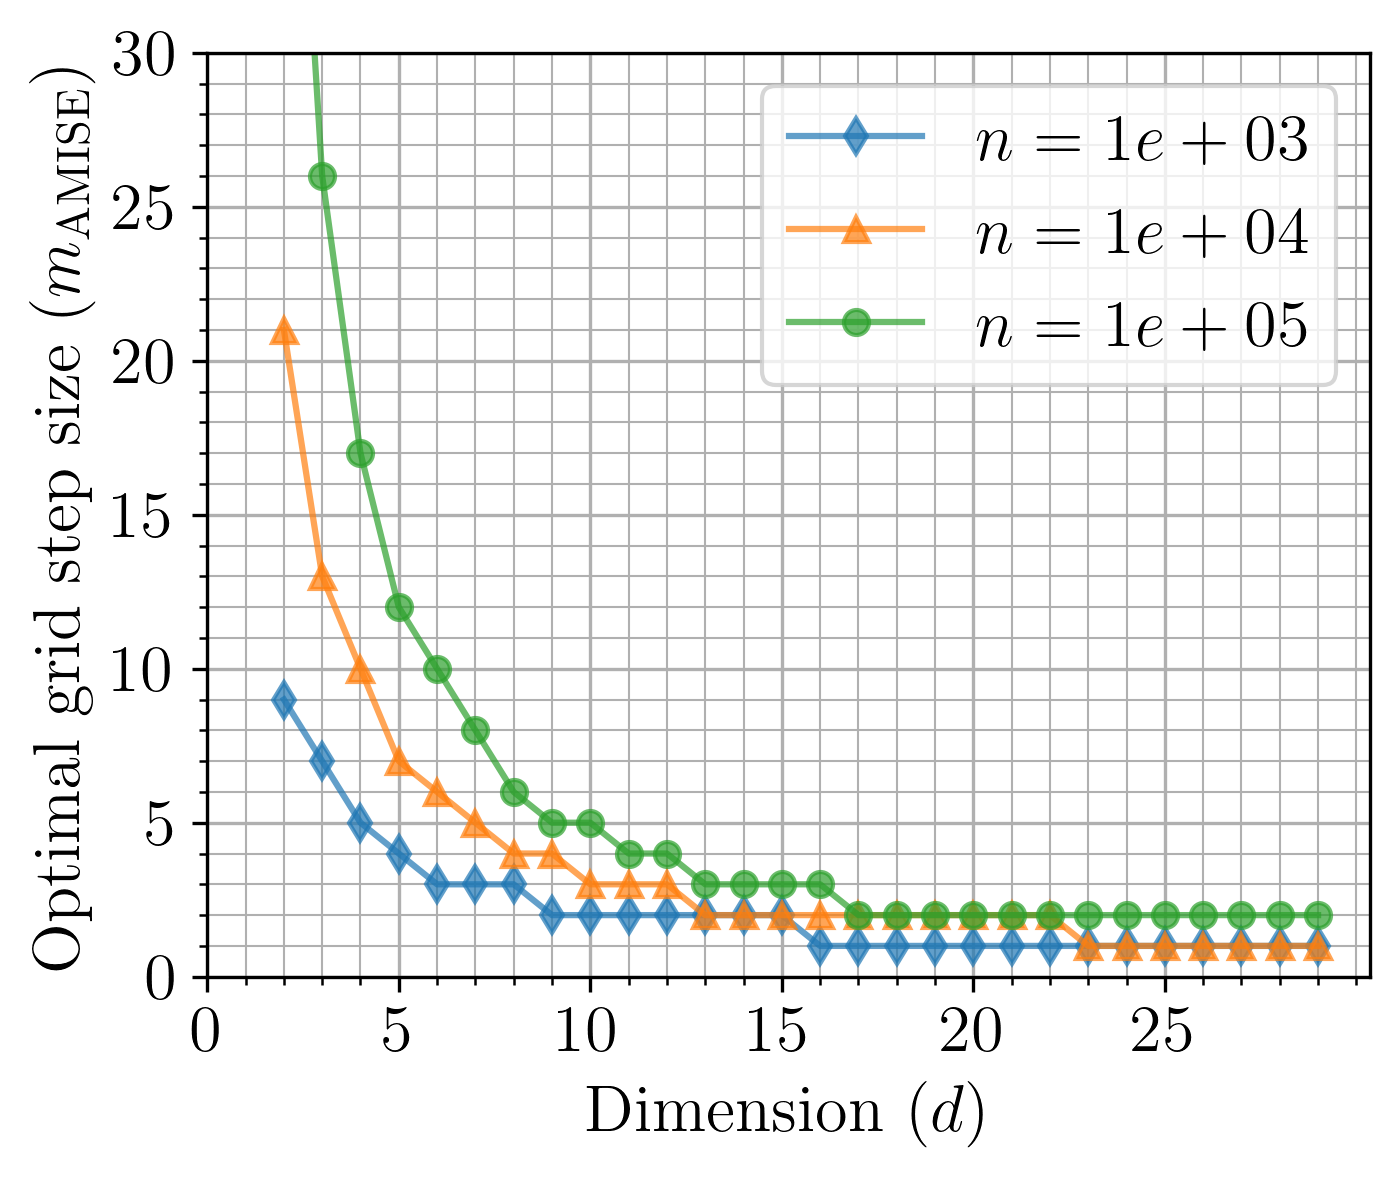
\includegraphics[width=0.5\linewidth]{../numerical_experiments/chapter3/figures/hAMISE.png}
    \caption{Evolution of $m_{\mathrm{IMSE}}$ for different dimensions and sample sizes.}
    \label{fig:hmise}
\end{figure}

The polynomial order for EBC estimation is still a bottleneck that was studied over the years by different authors (see e.g., \citealt{janssen_2012_ebc,bouezmarni_2013_EBC_convergence,rose_2015,segers_2017}).  
Meanwhile, other nonparametric approaches such as the ``penalized Bernstein'' and the ``penalized B-spline'' estimators were compared to the EBC and vine copulas in a benchmark realized by \citet{nagler_2017}. 
The results showed that the most performant methods vary depending on the problem studied (for different dimensions, sample sizes, and strength of dependence). 
Regarding tail dependence modeling, nonparametric approaches are generally limited, but recent contributions introduced Bootstrap procedures to better this aspect \citep{kiriliouk_2021_resampling}.


\subsubsection{Illustrative example on a Clayton copula}
%------------------------------------------------------------%
Let us consider a bivariate Clayton copula $C$ with parameter $\theta=2.5$ (see \citealt{nelsen_2006_copulas})
A Monte Carlo sample with size $n=10$ is generated on it, which is then used to build an empirical copula $C_n$ as defined in \eq{eq:empirical_copula}. 
\fig{fig:ebc_illustration} (a) illustrates the empirical copula corresponding to the sample, with the shade of grey matching the CDF values. 
Then, the Bernstein approximation of the empirical copula (i.e., the EBC)  is represented in \fig{fig:ebc_illustration} (b), (c), (d) according to the \eq{eq:ebc}. 
The three versions of the EBC correspond to different polynomial orders, assuming that $(m_1=m_2)$. 

As the order increases, the bias between the EBC and the copula $C$ tends to be reduced. 
Note that the second EBC in \fig{fig:ebc_illustration} (c) where $(m_1=m_2=n)$ is equivalent to the Beta copula. 
Moreover, increasing the order beyond the sample size definitely overfits the copula. 

%\elias{possible alternative: 2D plots in two rows. Row 1: empirical copula/EBCn=5/EBCn=10. Row 2: empirical density copula/EBCn=5/EBCn=10.}

\begin{figure}
    \begin{subfigure}[b]{0.49\textwidth}
        \centering
        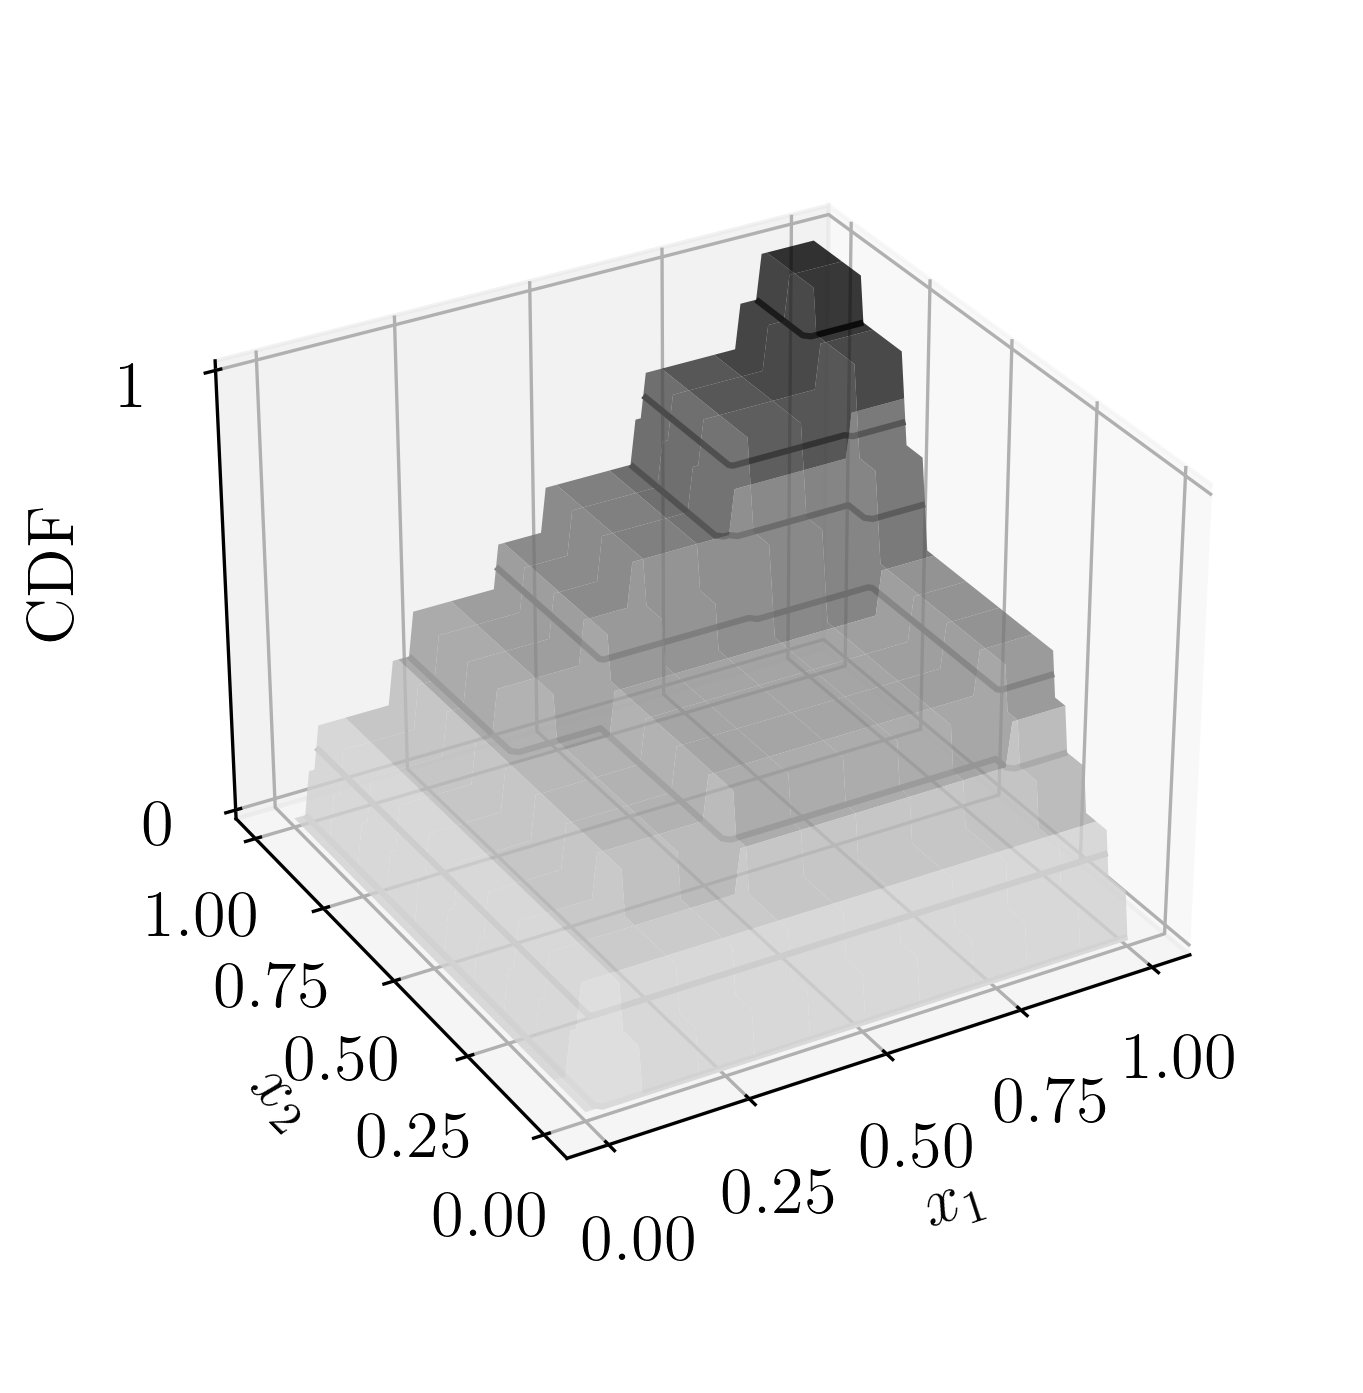
\includegraphics[width=\linewidth]{../numerical_experiments/chapter3/figures/empirical_copula.png}
        \caption{Empirical copula $C_n$ with ($n=10$).}
    \end{subfigure}
    \begin{subfigure}[b]{0.49\textwidth}
        \centering
        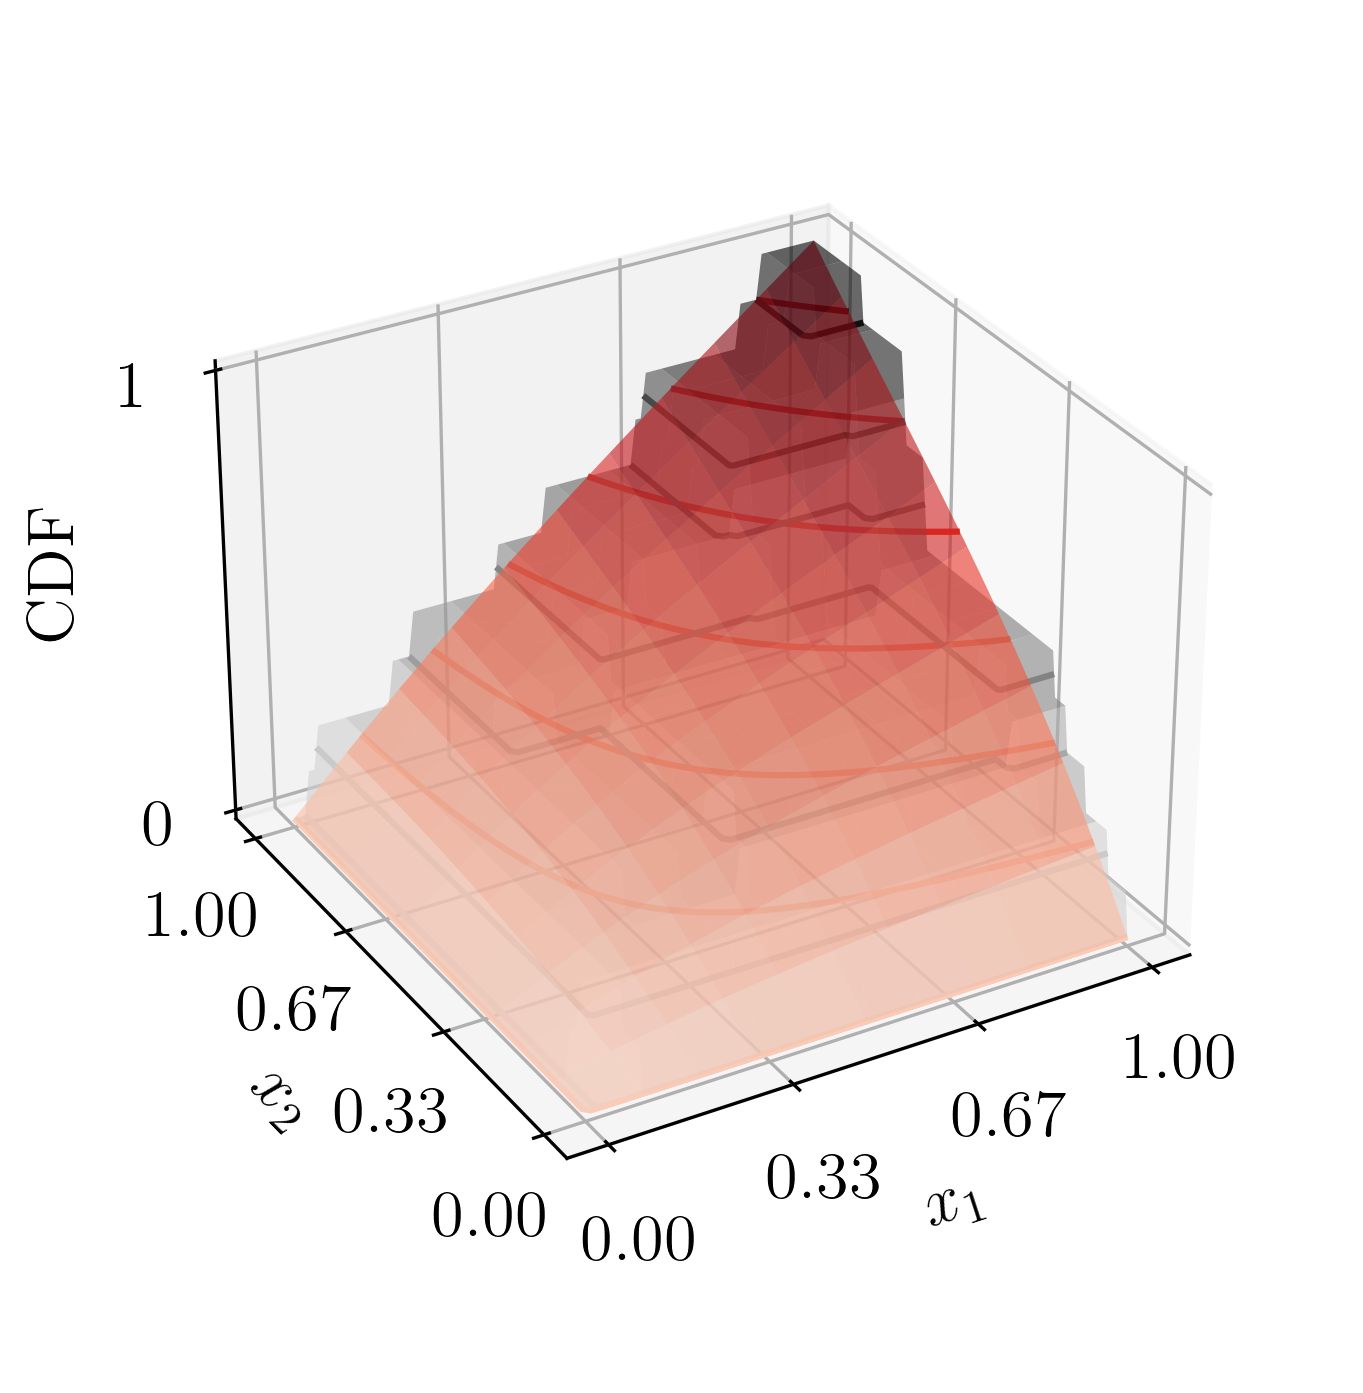
\includegraphics[width=\linewidth]{../numerical_experiments/chapter3/figures/ebc_m3.png}
        \caption{$B_{\bm}(C_n)$ with $(m_1=m_2=3)$.}
    \end{subfigure}
    \\
    \begin{subfigure}[b]{0.49\textwidth}
        \centering
        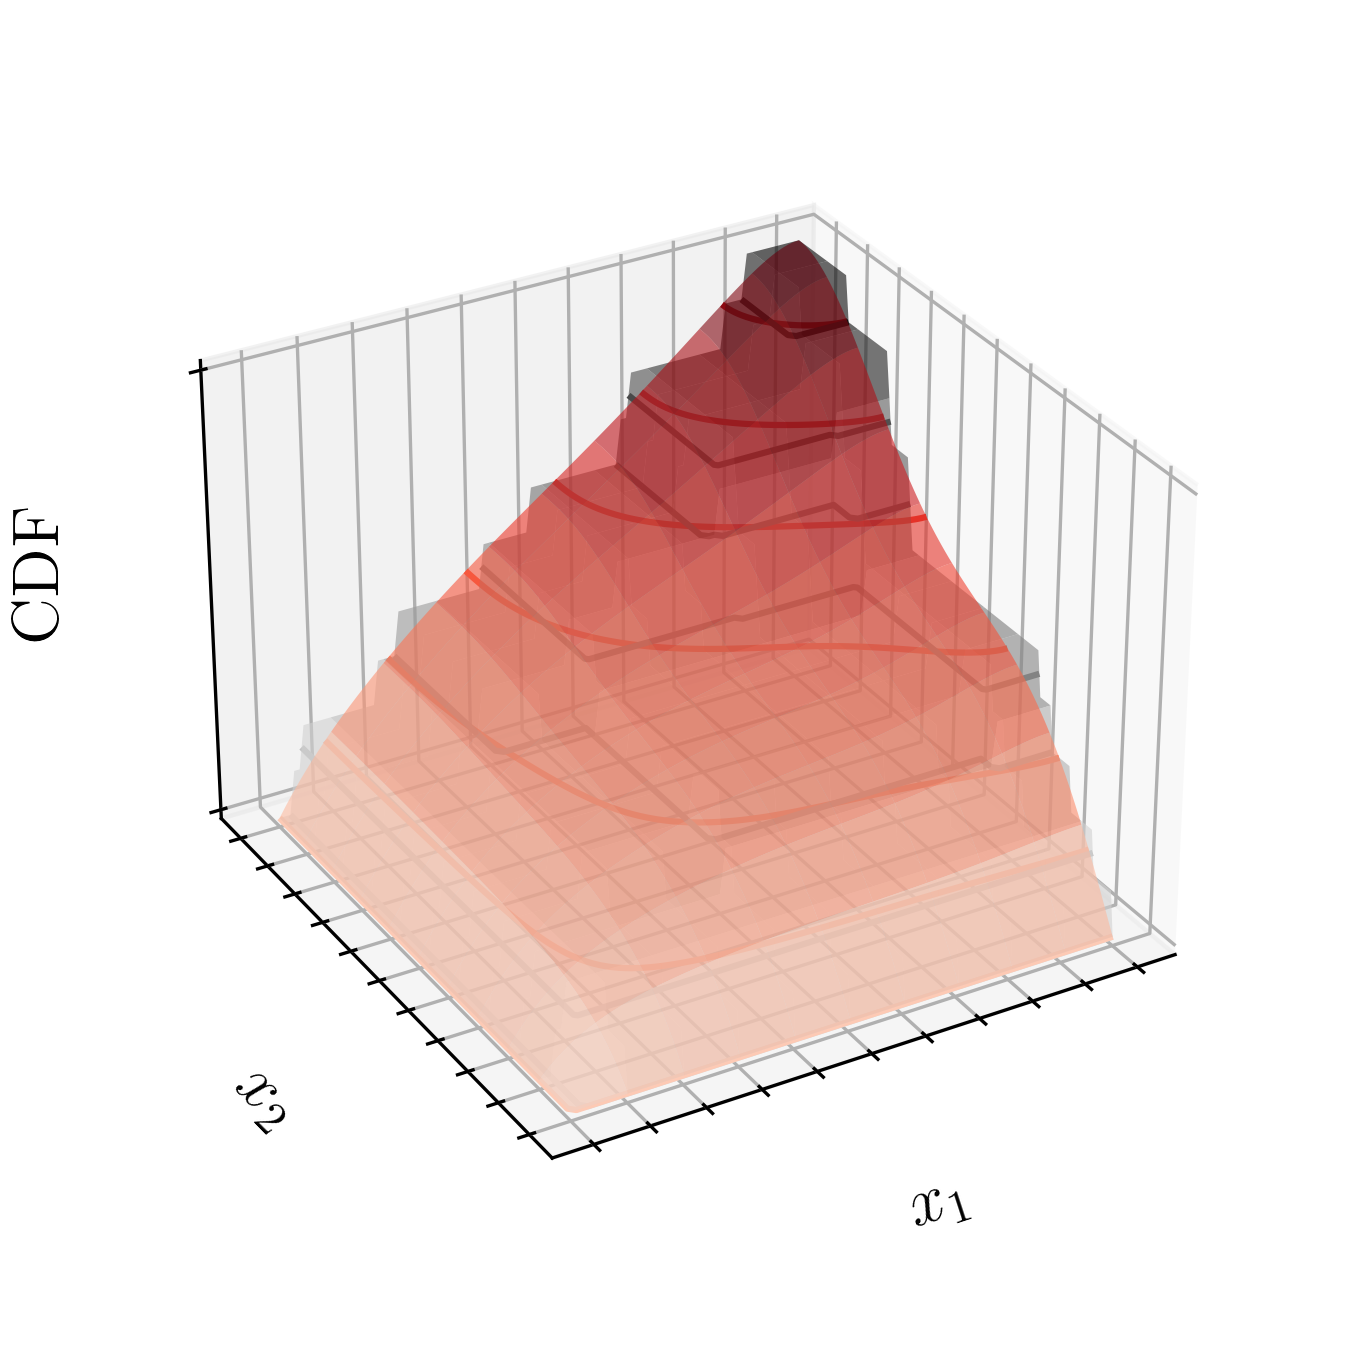
\includegraphics[width=\linewidth]{../numerical_experiments/chapter3/figures/ebc_m10.png}
        \caption{$B_{\bm}(C_n)$ with $(m_1=m_2=10)$.}
    \end{subfigure}
    \begin{subfigure}[b]{0.49\textwidth}
        \centering
        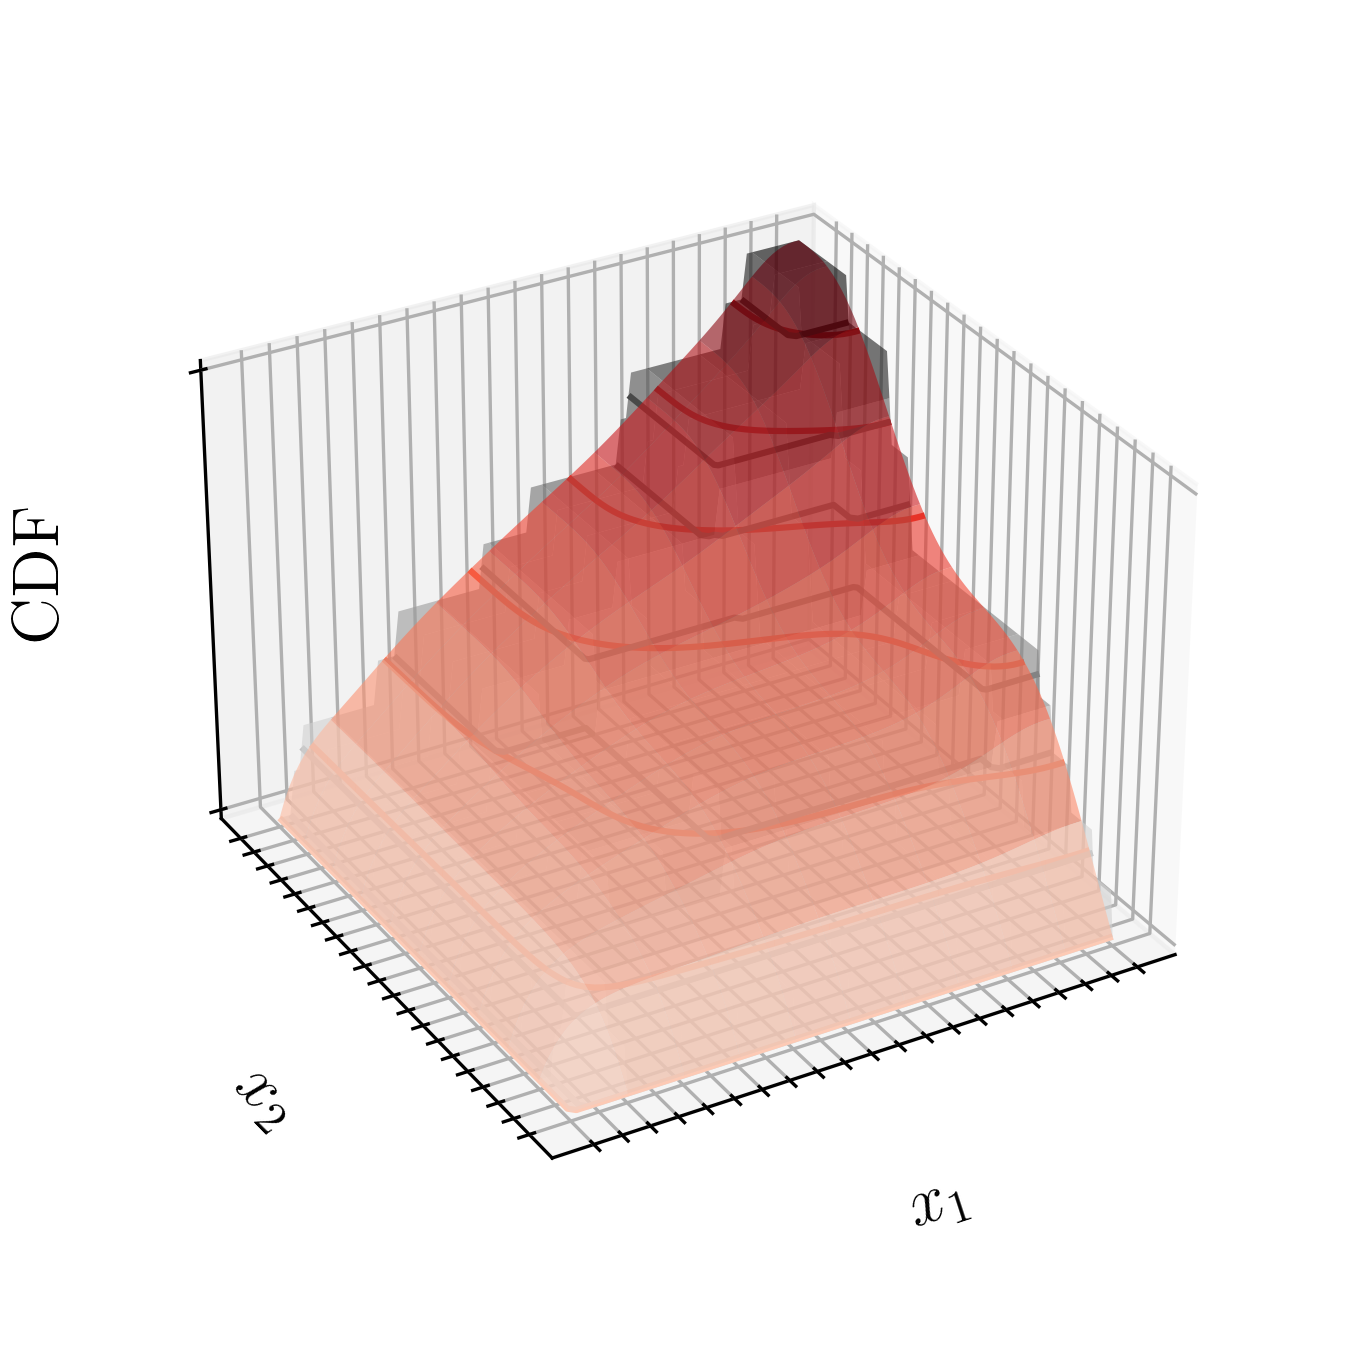
\includegraphics[width=\linewidth]{../numerical_experiments/chapter3/figures/ebc_m20.png}
        \caption{$B_{\bm}(C_n)$ with $(m_1=m_2=20)$.}
    \end{subfigure}
    \centering
    \caption{Bernstein approximations of the empirical copula $C_n$ (with size $n=10$) of a Clayton copula (with parameter $\theta=2.5$). The polynomial orders are assumed equal in the two dimensions $m_1=m_2\in\{3, 10, 20\}$.}
    \label{fig:ebc_illustration}
\end{figure}

\newpage
%============================================================%
%============================================================%
\section{\textit{Copulogram}: a tool for multivariate data visualization}\label{sec:copulogram}
%============================================================%
%============================================================%
In statistics, data visualization offers a wide set of tools to analyze data. 
Multivariate data visualization is of great help in apprehending problems with dimensions higher than two. 
In the context of continuous variables, let us consider the $n$-sized sample $\bX_n = \left\{\bx^{(1)}, \dots, \bx^{(n)}\right\} \sim \bX \in \iD_{\bx}\subseteq\R^d$. 
The marginal samples of $\bX_n$ are denoted by $X_{n, j} = \{x_j^{(1)}, \dots, x_j^{(n)}\}, j\in \{1, \dots, d\}$.

Various techniques exist to represent multivariate data, such as the ``parallel coordinate plot'', also called ``cobweb plot'' (see e.g., \citealp{heinrich_2013_cobweb}). 
For each sample $\bx^{(i)} \in \bX_n$, this plot draws a line passing by the values of $\bx^{(i)} = [x_1^{(i)}, \dots, x_d^{(i)}]$. 
This representation was used in sensitivity analysis to illustrate the connections between a set of inputs and an output, however, it does not provide a good representation of the dependence structure between the inputs. 

%============================================================%
\subsection{From the pairwise plot to the copulogram}
%============================================================%
Alternatively, the ``pairwise plot'', also named ``generalized draftsman plot'', was initially introduced by \citet{hartigan_1975_splom} to draw a matrix of scatter-plots between all the pairs of marginal samples $\{X_{n, i}, X_{n, j}\}, i \ne j \in \{1, \dots, d\}^2$. 
Because of the symmetry, the pairwise plot is usually represented on the lower triangle of the matrix. 
Later on, statisticians improved the pairwise plot by adding a histogram (or KDE) of the marginal samples $X_{n, j} j \in \{1, \dots, d\}$ on the diagonal. 
Additionally, the upper triangle was completed with the values of linear correlation for each pair of marginal samples $\{X_{n, i}, X_{n, j}\}, i \ne j$. 
This matrix of correlation coefficients is also known as ``correlogram''. 
Altogether, this matrix plot became known as the ``scatter plot of matrices'' (SPLOM). 

However, the linear correlation coefficient is known to give a poor description of the dependence in nonlinear cases. 
When analyzing a continuous sample $\bX_n \sim \bX$, the Sklar theorem states that the dependence structure within the random vector $\bX$ has a unique expression with its $d$-copula $C$. 
As mentioned in Section~\ref{sec:copula_prelims}, the component-wise normalized ranks of the original sample $\bX_n$ define the empirical copula density $c_n$ (converging towards $C$ as $n$ increases).

To the best of our knowledge, the \textit{copulogram} is a new multivariate data visualization tool improving the SPLOM by representing the empirical copula density $c_n$ on the upper triangle of the matrix plot. 
This plot is an empirical decomposition of a multivariate sample in the vein of the Sklar theorem between marginals on the diagonal and copula on the upper triangle.

%============================================================%
\subsection{Implementation in a Python package}
%============================================================%

An open-source implementation is proposed in the python package \href{https://github.com/efekhari27/copulogram}{\texttt{copulogram}}. 
This code mostly relies on the Python package for data visualization \href{https://seaborn.pydata.org/}{\texttt{seaborn}} \citep{waskom_2021_seaborn}. 
The developments are tracked and archived in a GitHub repository\footnotemark and the package can be installed from the package-management system ``PyPI''. 

Multiple visual options are offered by the \texttt{copulogram} package, as illustrated in the GitHub repository. 
For example, the user can represent the univariate samples on the diagonal or the bivariate samples in the triangles with kernel density estimation.  
Categorical variables can be used to assign different colors depending on the data class. 
The colors can also vary depending on a continuous variable after defining a mapping between the values of this variable and a set of colors (also called colorbar).


\footnotetext{GitHub repository: \url{https://github.com/efekhari27/copulogram}}




\subsubsection{Example \#1: Iris flower dataset}
%------------------------------------------------------------%

The first example illustrates the copulogram on a widely used dataset in the machine learning community. 
The iris flower dataset was first introduced by Fisher and became a reference dataset for classification techniques. 
In the following lines of Python code, the dataset is loaded and the copulogram package is used to draw the new plot. 
The resulting copulogram applied to the iris flower data is represented in \fig{fig:iris_copulogram}. 
\lstset{style=mystyle, language=python}
%
\begin{lstlisting}
    #!/usr/bin/python3        
    import seaborn as sns
    import copulogram as cp
    data = sns.load_dataset("iris")
    copulogram = cp.Copulogram(data)
    copulogram.draw(hue="species")
\end{lstlisting}
%
Since this data mostly presents linear dependencies, the copulogram is not very instructive. 
In other cases, the role of the dependence in the joint distribution is more important.



\subsubsection{Example \#2: Ishigami function}
%------------------------------------------------------------%

The Ishigami function is commonly used as a benchmark problem for global sensitivity analysis (GSA): 
\begin{equation}
    y = g(x_1, x_2, x_3) = \sin(x_1) + 7 \, \sin(x_2)^2 + \frac{x_3^4 \, \sin(x_1)}{10}.
\end{equation}
This uncertainty quantification problem considers an independent random input vector $\bX=\prod_{j=1}^{3} X_j$. 
While the marginals in GSA benchmarks are usually assumed to be uniform, they will be considered Gaussian hereafter to distinguish the different elements of the joint distribution. 
Therefore, let us define $X_j\sim \iN(0, 1) \forall j \in \{1, 2, 3\}$. 
In this setup, the random inputs are independent but they each present interesting dependencies with the random output $Y=g(\bX)$.

A Monte Carlo sample with size $n=10^3$ is generated, $\bX_n \simiid \bX$, and evaluated such that $Y_n=g(\bx_n)$.  
The copulogram of the input-output sample $(\bX_n, Y_n)$ is represented in \fig{fig:ishigami_copulogram}. 
As expected, the scatter plots between the inputs in the upper triangle are uniform (representing an independent density copula). 

In GSA, the work of \citet{poczos_2012_copulaMMD} studied the discrepancy between the empirical density copula $c_n(X_j, Y), j \in \{1, \dots, d\}$ and the independent copula to qualitatively assess the importance of $X_j$.  
In the same vein, the paper of \citet{plischke_2019_copulaGSA} attempted to formalize a link between different GSA approaches based on copulas and to quantitative approaches as the Sobol' indices. 

\begin{figure}
    \centering
    \quad\qquad\qquad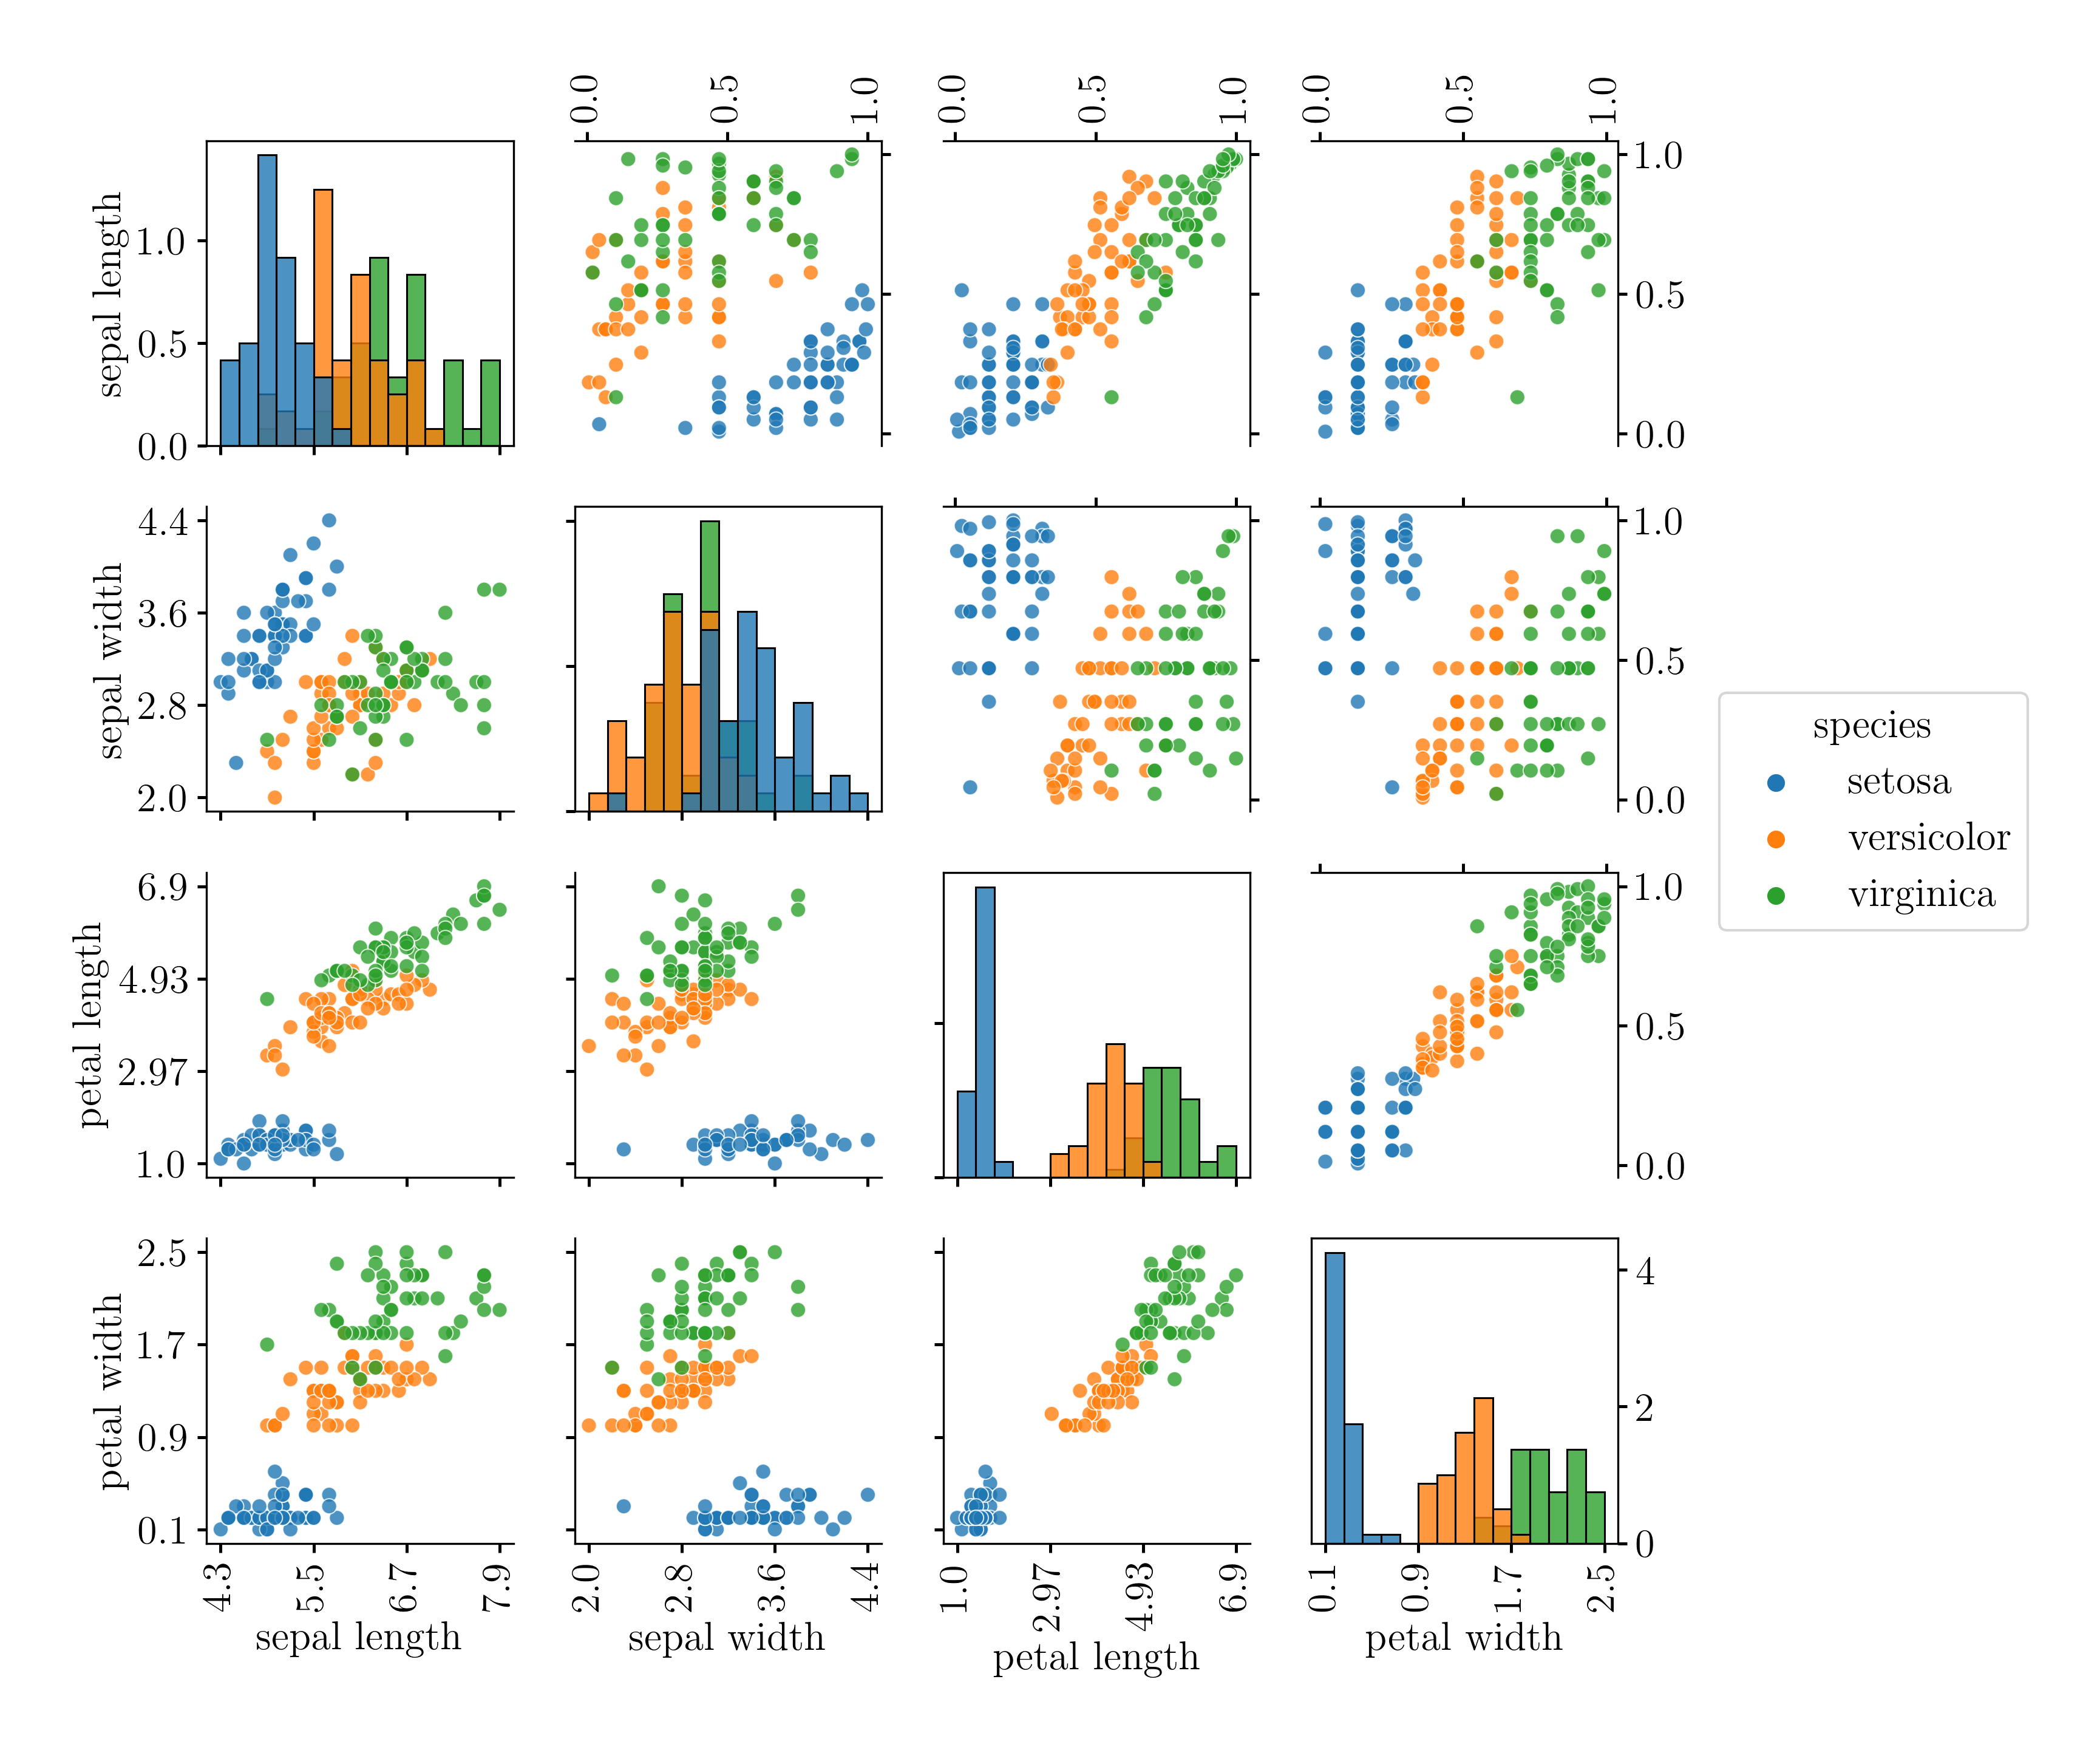
\includegraphics[width=0.82\textwidth]{../numerical_experiments/chapter3/figures/iris_copulogram.png}
    \caption{Copulogram of the iris flower dataset with colors assigned by the iris species.}
    \label{fig:iris_copulogram}
\end{figure}

\begin{figure}
    \centering
    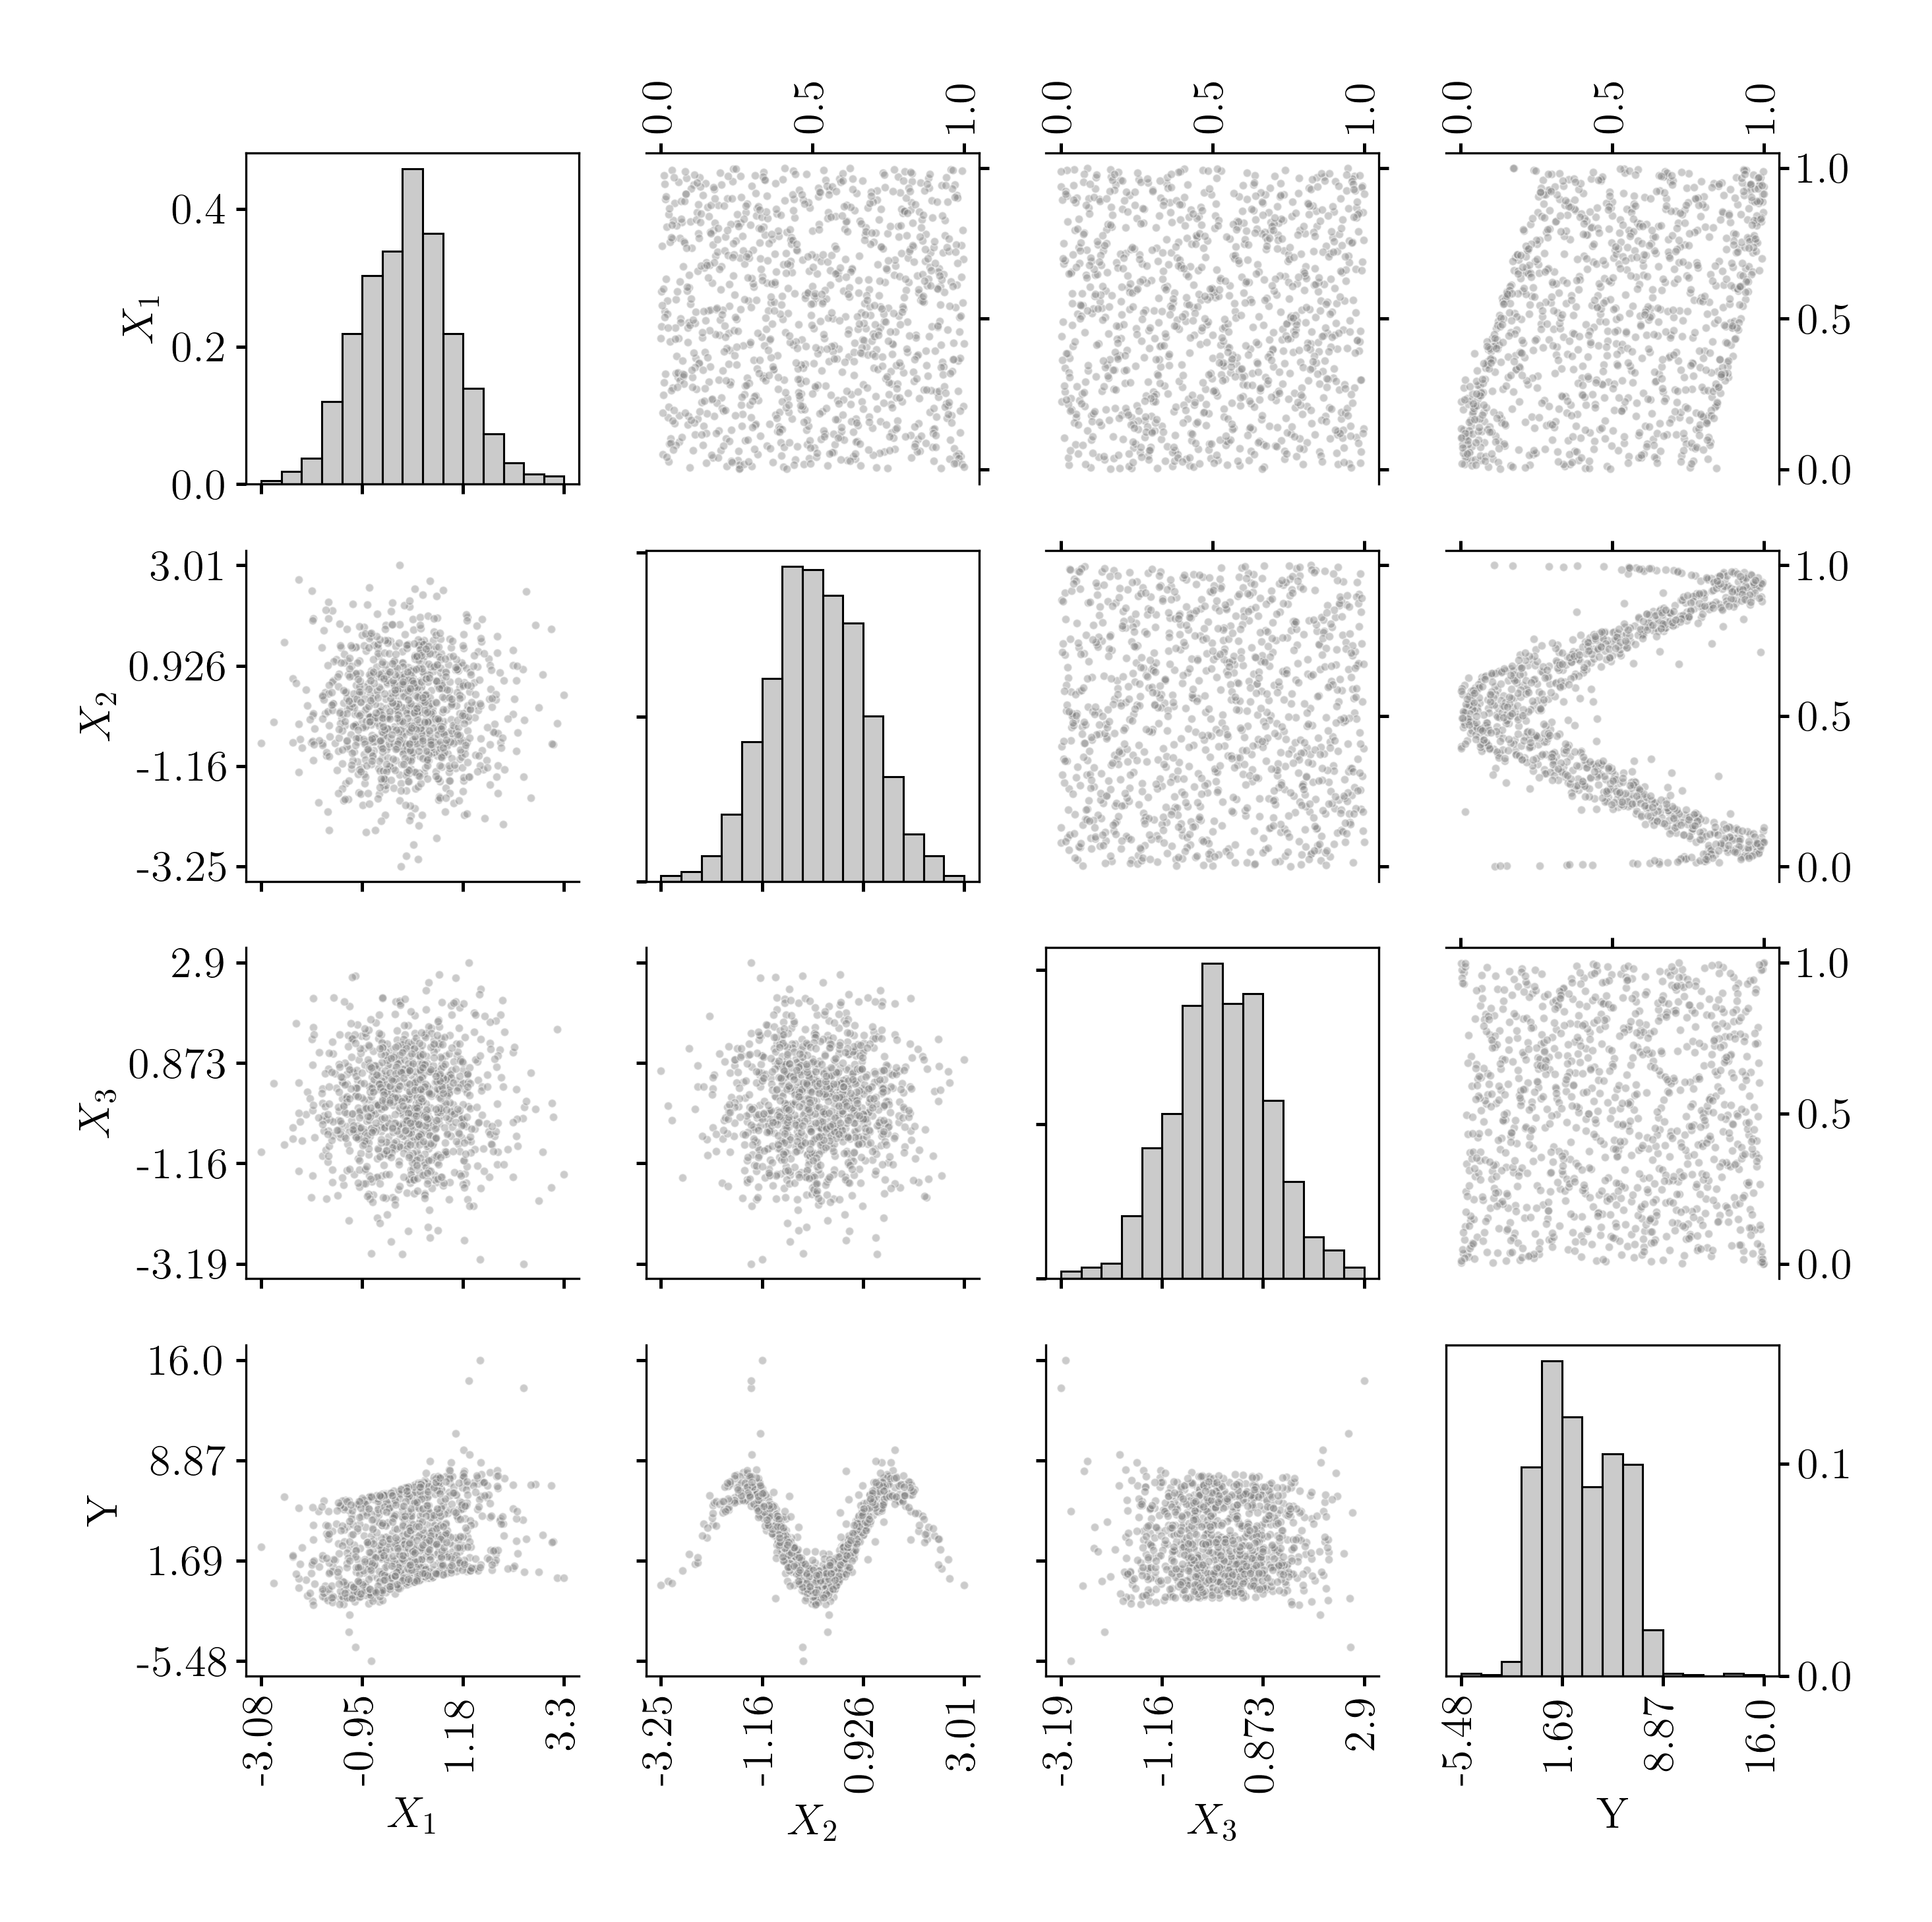
\includegraphics[width=0.7\textwidth]{../numerical_experiments/chapter3/figures/ishigami_copluogram.png}
    \caption{Copulogram of Monte Carlo sample (with size $n=10^3$) of the inputs and outputs of the modified Ishigami problem.}
    \label{fig:ishigami_copulogram}
\end{figure}



\newpage
%============================================================%
%============================================================%
\section{Semiparametric inference of the South Brittany metocean conditions} \label{sec:32_inference}
%============================================================%
%============================================================%
Metocean conditions have been long studied in coastal and offshore engineering. 
Inferring multivariate probabilistic models on metocean data became essential in wind energy. 

Numerous approaches are proposed in the literature to fit a model on environmental data. 
Among them, let us mention the use of parametric methods as the conditional modeling (e.g., \citealt{bitner_2015_joint,vanem_fekhari_2023}), or the construction of vine copulas (e.g., \citealt{vanem_2016,montes_2016_cvines_metocean,lin_2019_cvines_waves}). 
Nonparametric methods as the KDE were also applied in this context (e.g., \citealt{han_2018_kde_metocean}). 
The nonparametric techniques generally struggle to model the distributions' tails, even if the tails are essential to qualify structures for ultimate events. 
However, they are highly flexible and often easier to implement than parametric methods.

In this section, a semiparametric inference strategy is presented, composing some well-known parametric models for the marginals (e.g., Weibull distribution for the wind speed), with a highly flexible dependence modeling by the EBC. 
A metocean dataset is used to showcase the empirical Bernstein copula and its representation by the copulogram. 
This dataset from the ANEMOC (Digital Atlas of Ocean and Coastal Sea States atlas, \citealp{raoult_2018_anemoc3}) gathers 32 years of preprocessed data 
(at an hourly resolution) from a location off the coast of South Brittany, France. 
A subset of $10^4$ points is randomly selected among the ANEMOC data, which will be used to realize the semiparametric inference.
The full code developed for this inference study is available on a GitHub repository\footnotemark. 

\footnotetext{GitHub repository: \url{https://github.com/efekhari27/thesis/blob/main/numerical_experiments/chapter3/south_brittany_inference.ipynb}}

%============================================================%
\subsection{Inference of the marginals}\label{sec:marginal_inference}
%============================================================%

The variables studied to describe the environmental conditions match the ones defined in Table~\ref{tab:envi_variables}. 
Unfortunately, the turbulence is provided by the ANEMOC database and is therefore not fitted. 
A straightforward inference is performed on the data, resulting in the models presented in Table~\ref{tab:sb_marginal_fit}.
The wind and wave directions are fitted by KDE to catch their multimodal behavior while the other variables by MLE on various parametric models. 
Note that some variations of KDE with kernels specific to circular data could be interesting to ensure the continuity of the model at the bounds \citep{bai_1989_directional_kde}. 

The results of the marginals' inferences, plotted in \fig{fig:marginals_sb} against histograms, are visually satisfying. 
Statistical testing is not necessary in our case since the actual topic of discussion is related to the inference of the dependence. 
Considering these marginals, a study of the copula inference can be developed. 


\begin{table}
    \centering
    \begin{tabular}{llll}
        \hline
        {\it Name}              & {\it Notation}            & {\it Fitted model}                            & \textit{KS p-value ($\alpha$= 5\%)} \\
        \hline
        Wind speed              & $U$                       & Weibull ($\beta=11.4, \alpha=2.2, \gamma=0$)  & 0.238     \\
        Wind direction          & $\theta_{\mathrm{wind}}$  & KDE                                           & --        \\ 
        Significant wave height & $H_s$                     & Inverse Normal ($\mu=2.3, \lambda=6.8$)       & 0.533     \\
        Wave period             & $T_p$                     & Weibull ($\beta=9.3, \alpha=3.3, \gamma=2$)  & 0.00021   \\
        Wave direction          & $\theta_{\mathrm{wave}}$  & KDE                                           & --        \\
        \hline
    \end{tabular}
    \caption{Marginal inference results of the South Brittany metocean data.}
    \label{tab:sb_marginal_fit}
\end{table}

\begin{figure}
    \centering
    \begin{subfigure}[b]{0.32\textwidth}
        \centering
        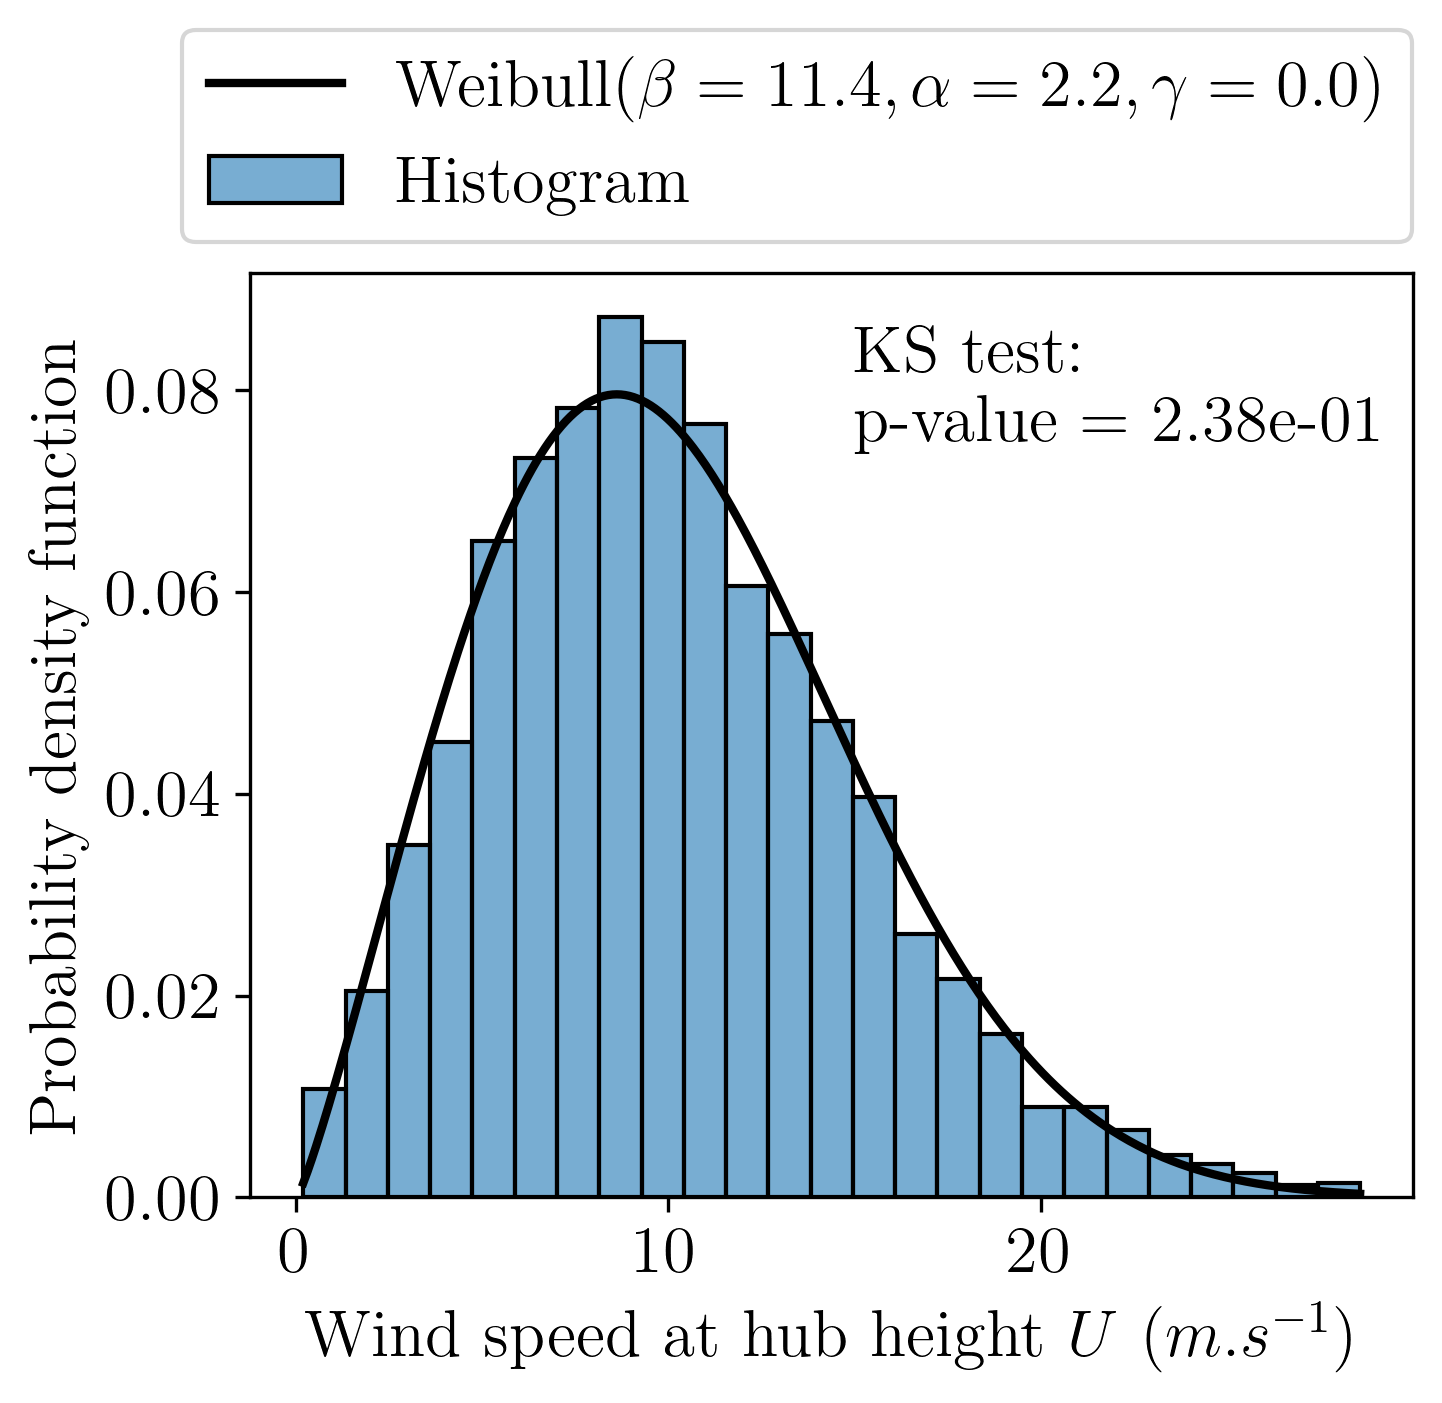
\includegraphics[width=\linewidth]{../numerical_experiments/chapter3/figures/free_wsp_distribution_SB.png}
        \caption{Wind speed $U$.}
    \end{subfigure}
    \begin{subfigure}[b]{0.32\textwidth}
        \centering
        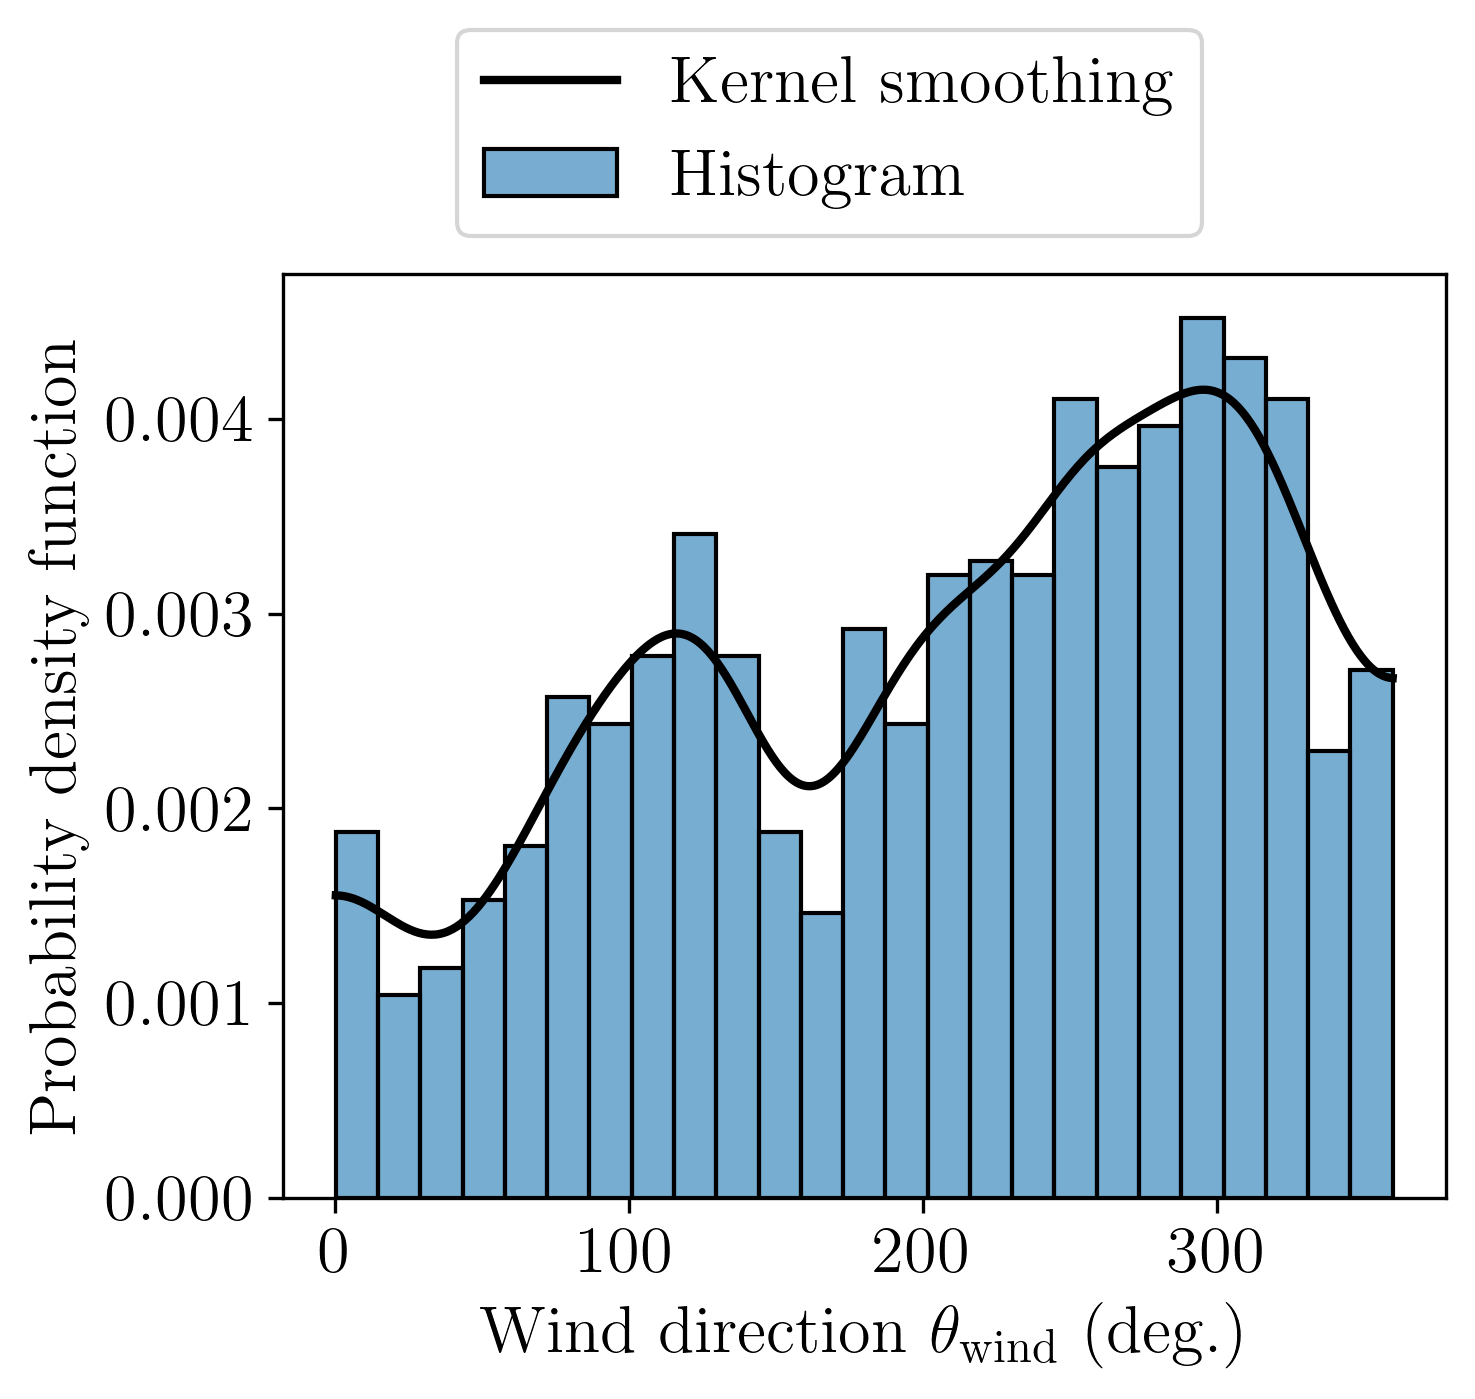
\includegraphics[width=\linewidth]{../numerical_experiments/chapter3/figures/wind_dir_distribution_SB.png}
        \caption{Wind direction $\theta_{\mathrm{wind}}$.}
    \end{subfigure}
    \\
    \begin{subfigure}[b]{0.32\textwidth}
        \centering
        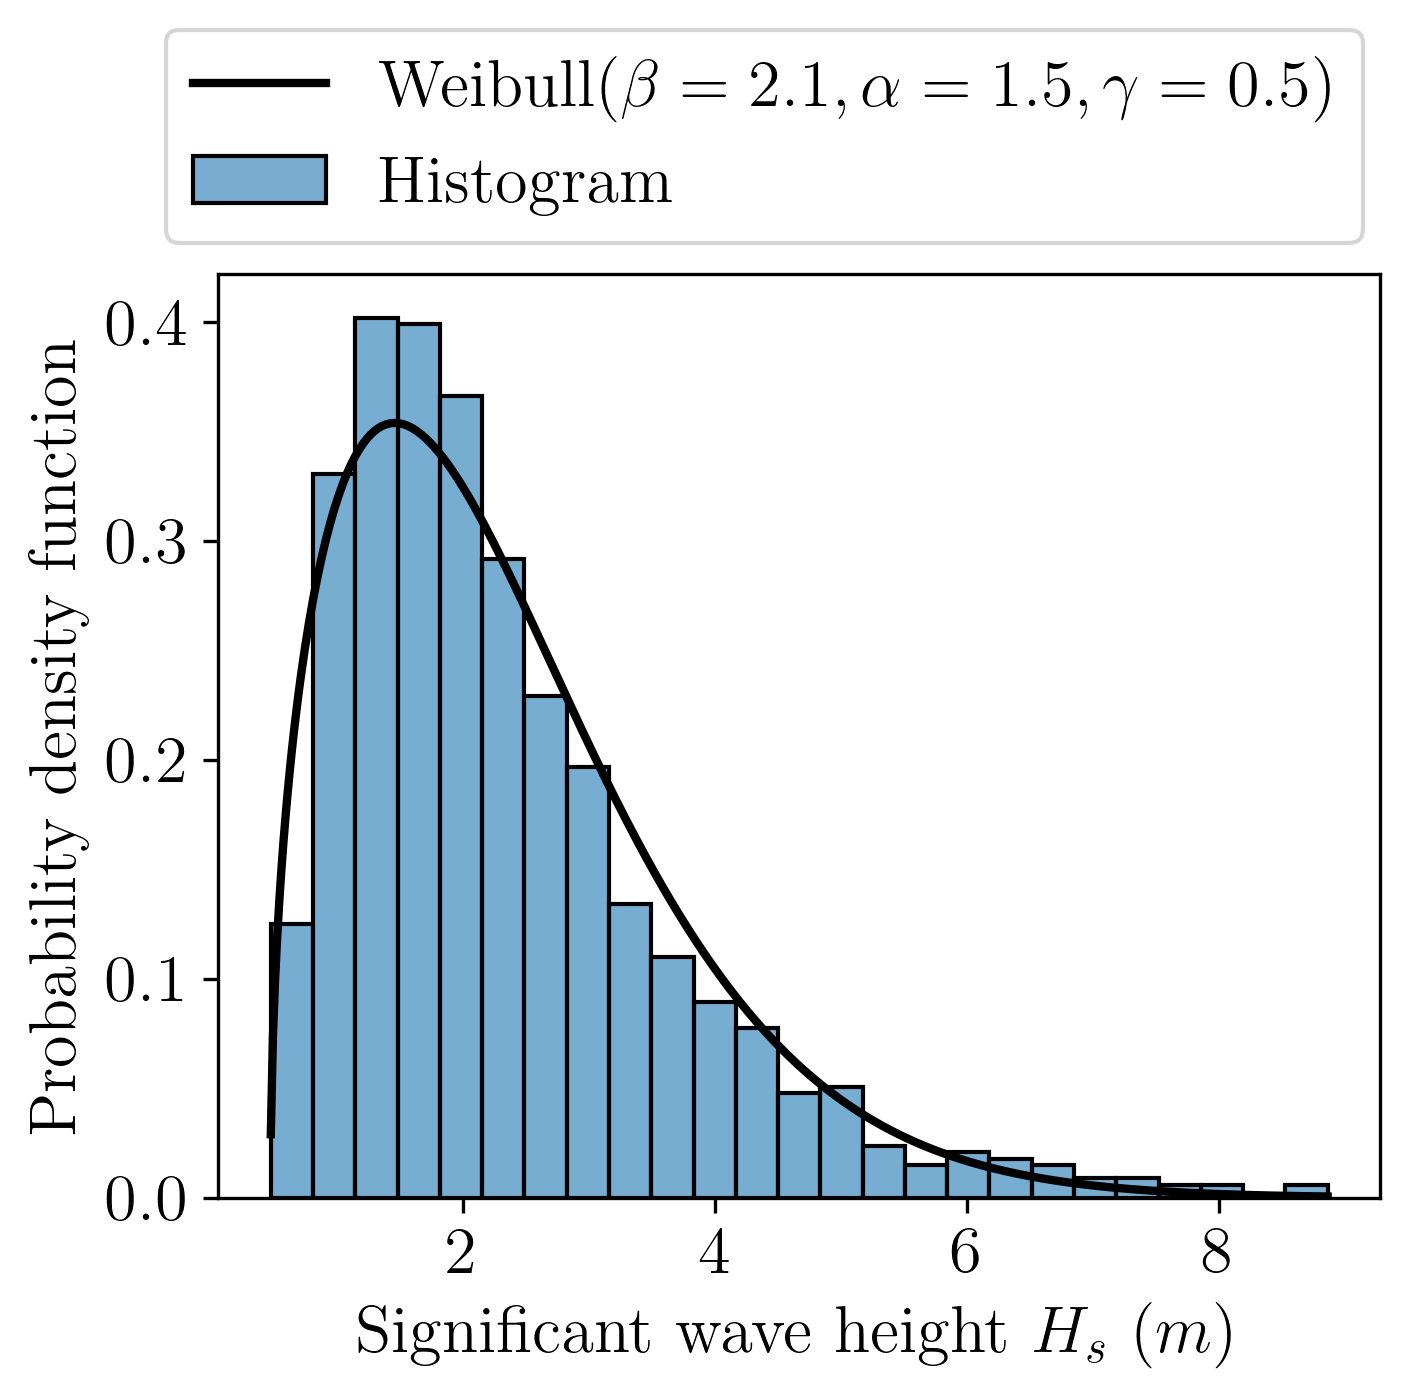
\includegraphics[width=\linewidth]{../numerical_experiments/chapter3/figures/Hs_distribution_SB.png}
        \caption{Significant wave height $H_s$.}
    \end{subfigure}
    \begin{subfigure}[b]{0.32\textwidth}
        \centering
        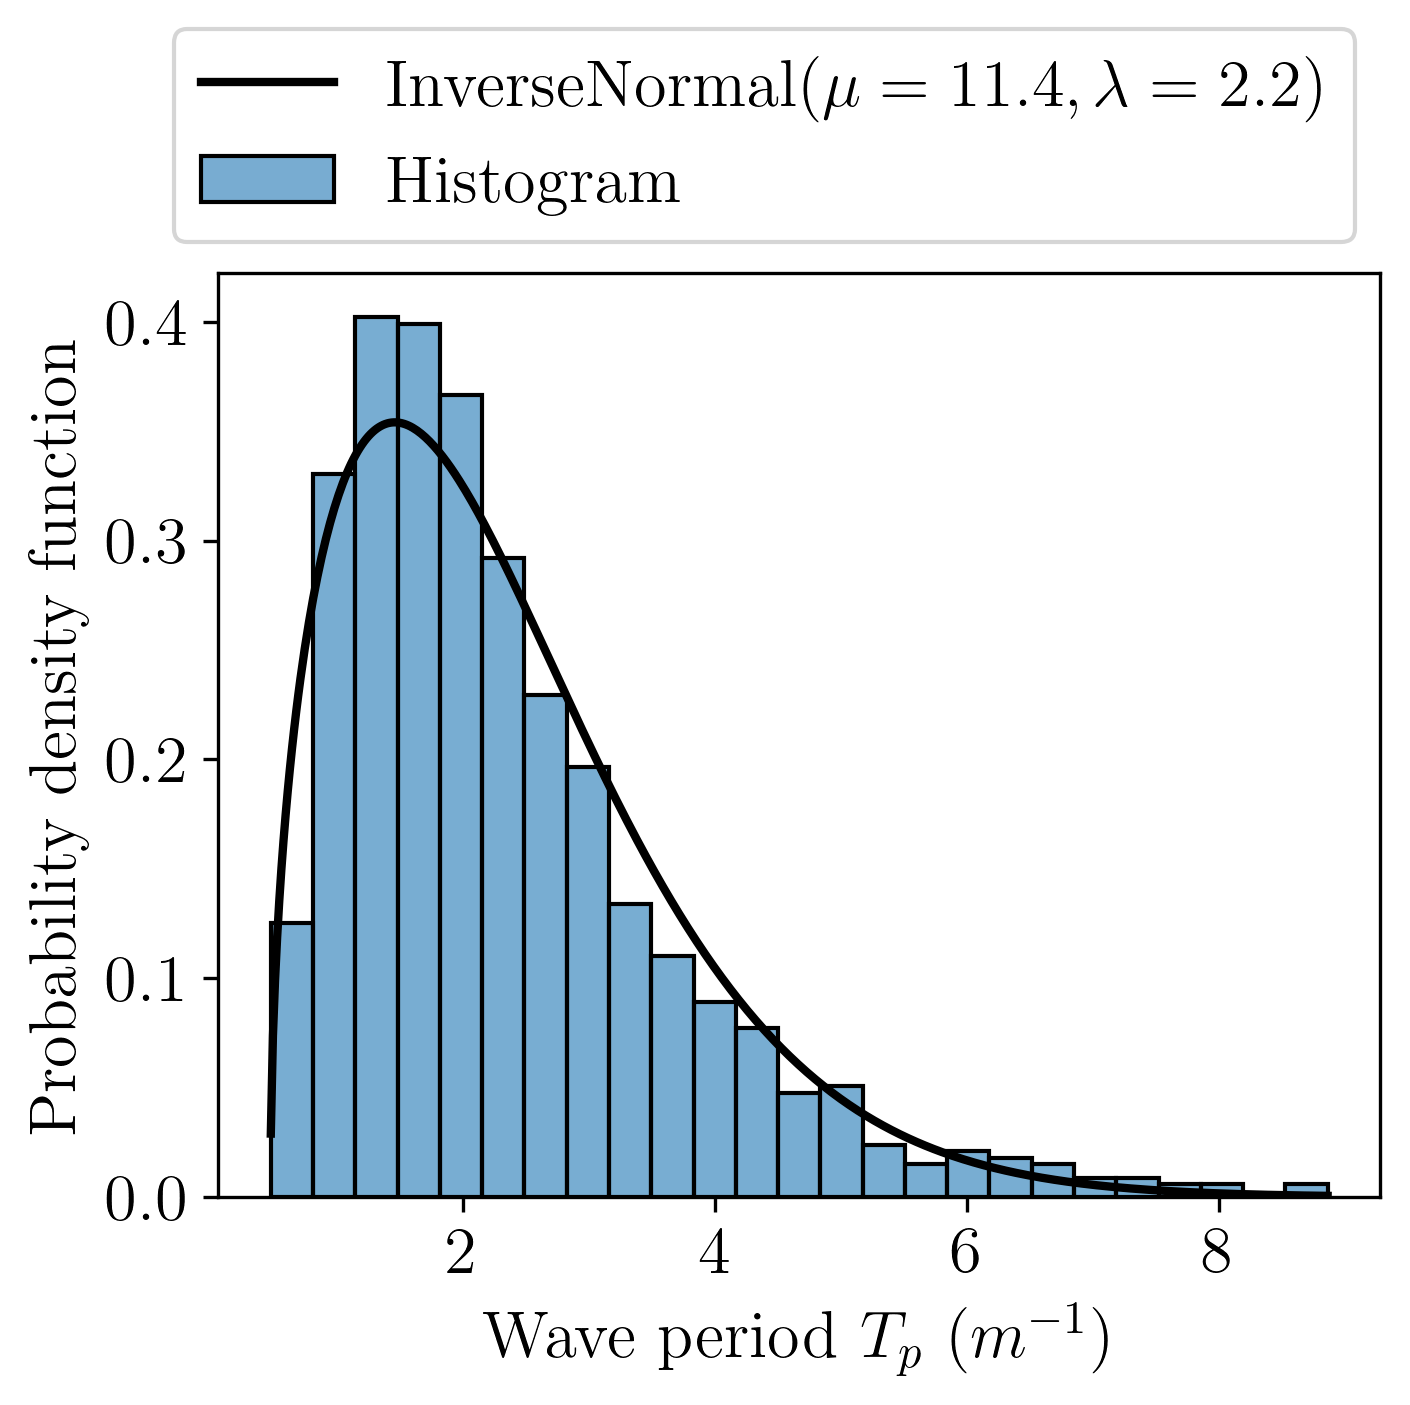
\includegraphics[width=\linewidth]{../numerical_experiments/chapter3/figures/Tp_distribution_SB.png}
        \caption{Wave period $T_p$.}
    \end{subfigure}
    \begin{subfigure}[b]{0.32\textwidth}
        \centering
        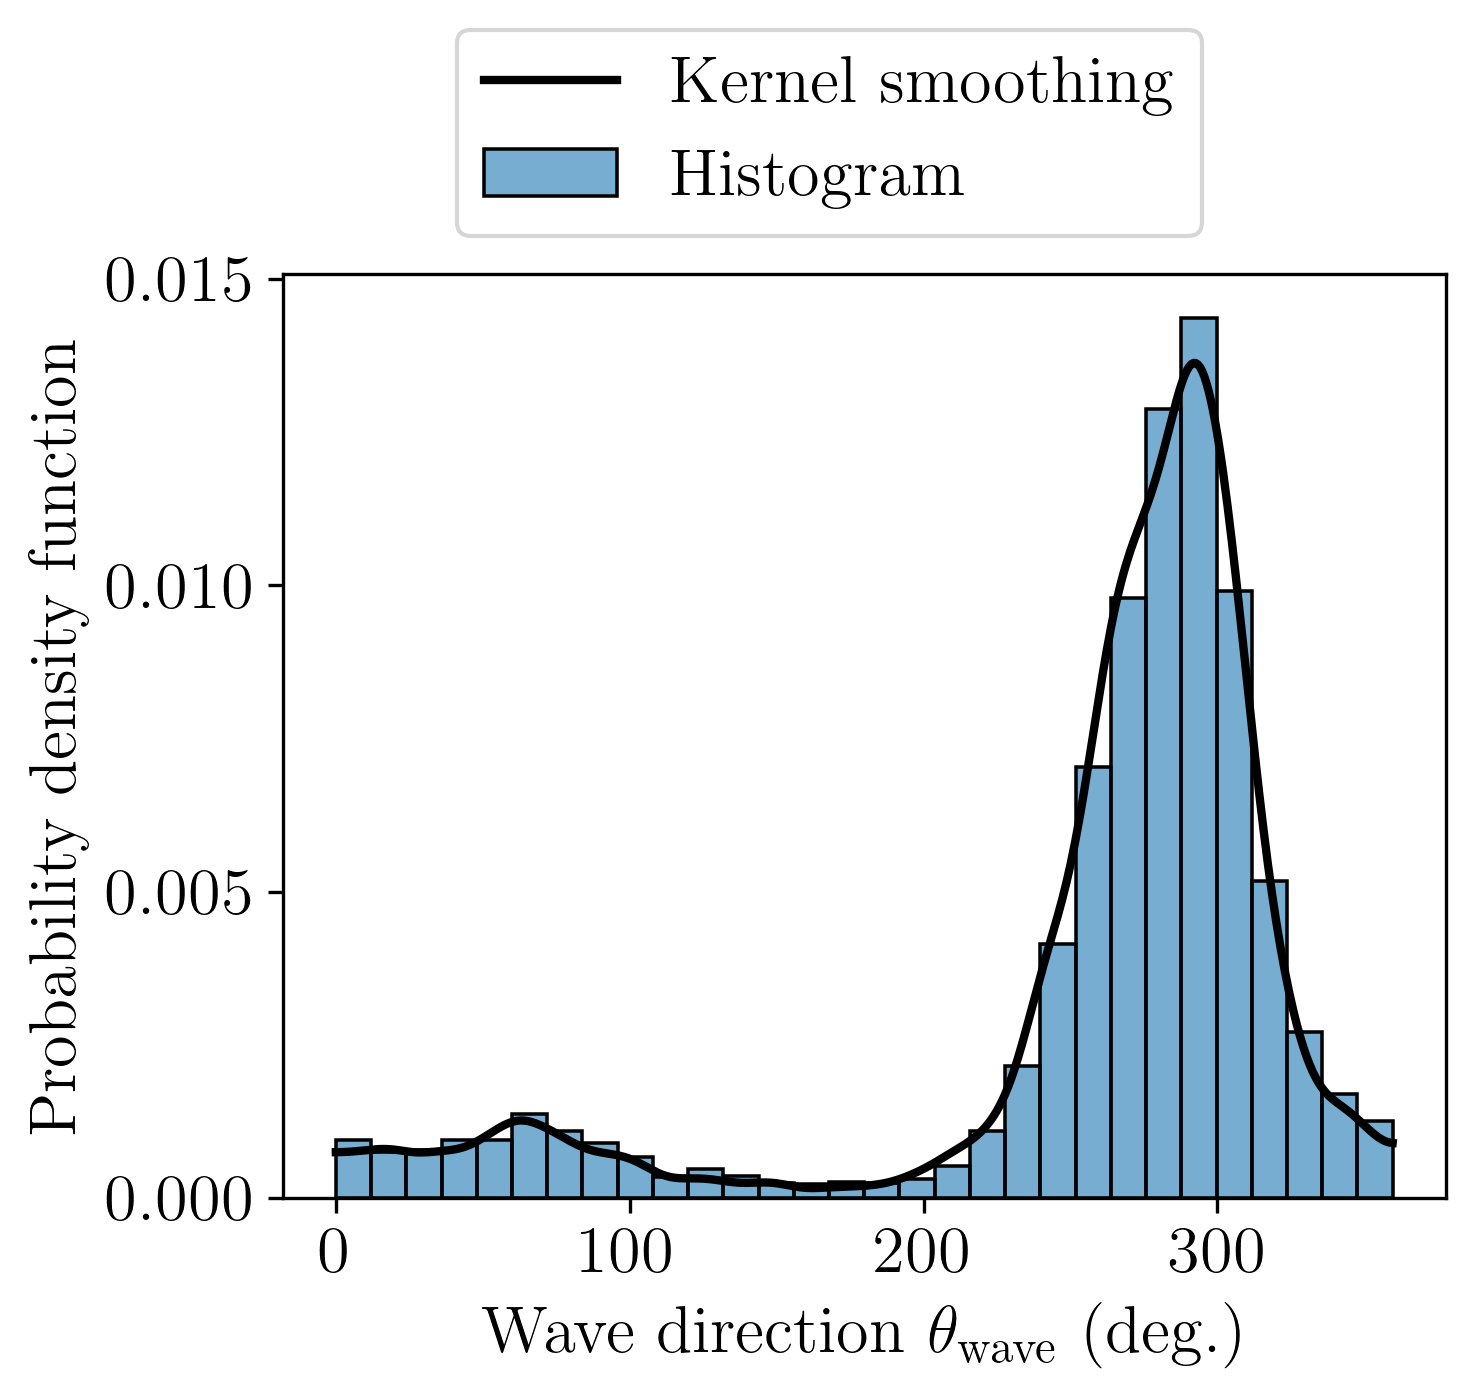
\includegraphics[width=\linewidth]{../numerical_experiments/chapter3/figures/wave_dir_distribution_SB.png}
        \caption{Wave direction $\theta_{\mathrm{wave}}$.}
    \end{subfigure}
    \caption{Marginal inference results of the South Brittany metocean data.}
    \label{fig:marginals_sb}
\end{figure}

\newpage
%============================================================%
\subsection{Nonparametric inference of the dependence}
%============================================================%

The aim of this section is to complete the set of marginals fitted previously by the inference of a copula. 
A nonparametric estimation using the empirical Bernstein copula is studied in this section. 
To validate the goodness-of-fit of the EBC, the ANEMOC dataset (with size $N=10^4$) is randomly split into two:
a learning set $\bX_n$ and a validation set $\bX_n'$. 
A joint distribution $\what{F_\bX}$ is then build using $\bX_n$, by combining the marginals fitted earlier with an empirical copula $B_{\bm}(C_n)$, such that: 
\begin{equation}
    \what{F_\bX}(\bx) = B_{\bm}(C_n)\left(\what{F_{X_1}}(x_1), \dots, \what{F_{X_d}}(x_d)\right).
\end{equation}
Where $\what{F_{X_j}}$ stand for the model of the marginal $j$, just inferred in Section~\ref{sec:marginal_inference}. 
While $C_n$ is the empirical copula associated with the sample $\bX_n$, and all the polynomial orders of the EBC are equal, $\bm = \{m, \dots, m\}, m\in\N$.

Then, one could compare a sample $\what{\bX_n}$, generated from the fitted joint distribution $\what{F_\bX}$, with the learning set $\bX_n$. 
However, to prevent an overfit from the semiparametric model, the comparison is rather done between $\bX_n$ and the independent validation set $\bX_n'$. 
The statistic used is the maximum mean discrepancy, $\MMD(\what{\bX_n}, \, \bX_n')$, initially introduced for multivariate two-sample testing (a specific presentation of the MMD and its estimation is developed in Appendix~\ref{apx:B}). 
For a given fitted joint distribution, this procedure is repeated 100 times to take into account the sampling variability. 

In \fig{fig:sb_ebc_mmd}, MMD distributions are represented for different values of the EBC polynomial order, with $m\in\{5, 10, 20, 50, 100, 1000\}$. 
The smaller the values of this dissimilarity measure, the closer the samples should be. 
Even if further developments could be implemented to improve the MMD estimation, these results are sufficient to set the EBC tuning at $m=100$. 
Considering this setup, \fig{fig:sb_copulograms} represents the copulogram of a sample $\what{\bX_n}$ (in red), side by side with the copulogram of the learning set $\bX_n$ (in blue).  
This semiparametric approach offers a lot of flexibility, which is essential when inferring such complete dependence structures. 
As with any nonparametric method, it should be used with caution when inferring distributions' tails.  


\begin{figure}[h]
    \centering
    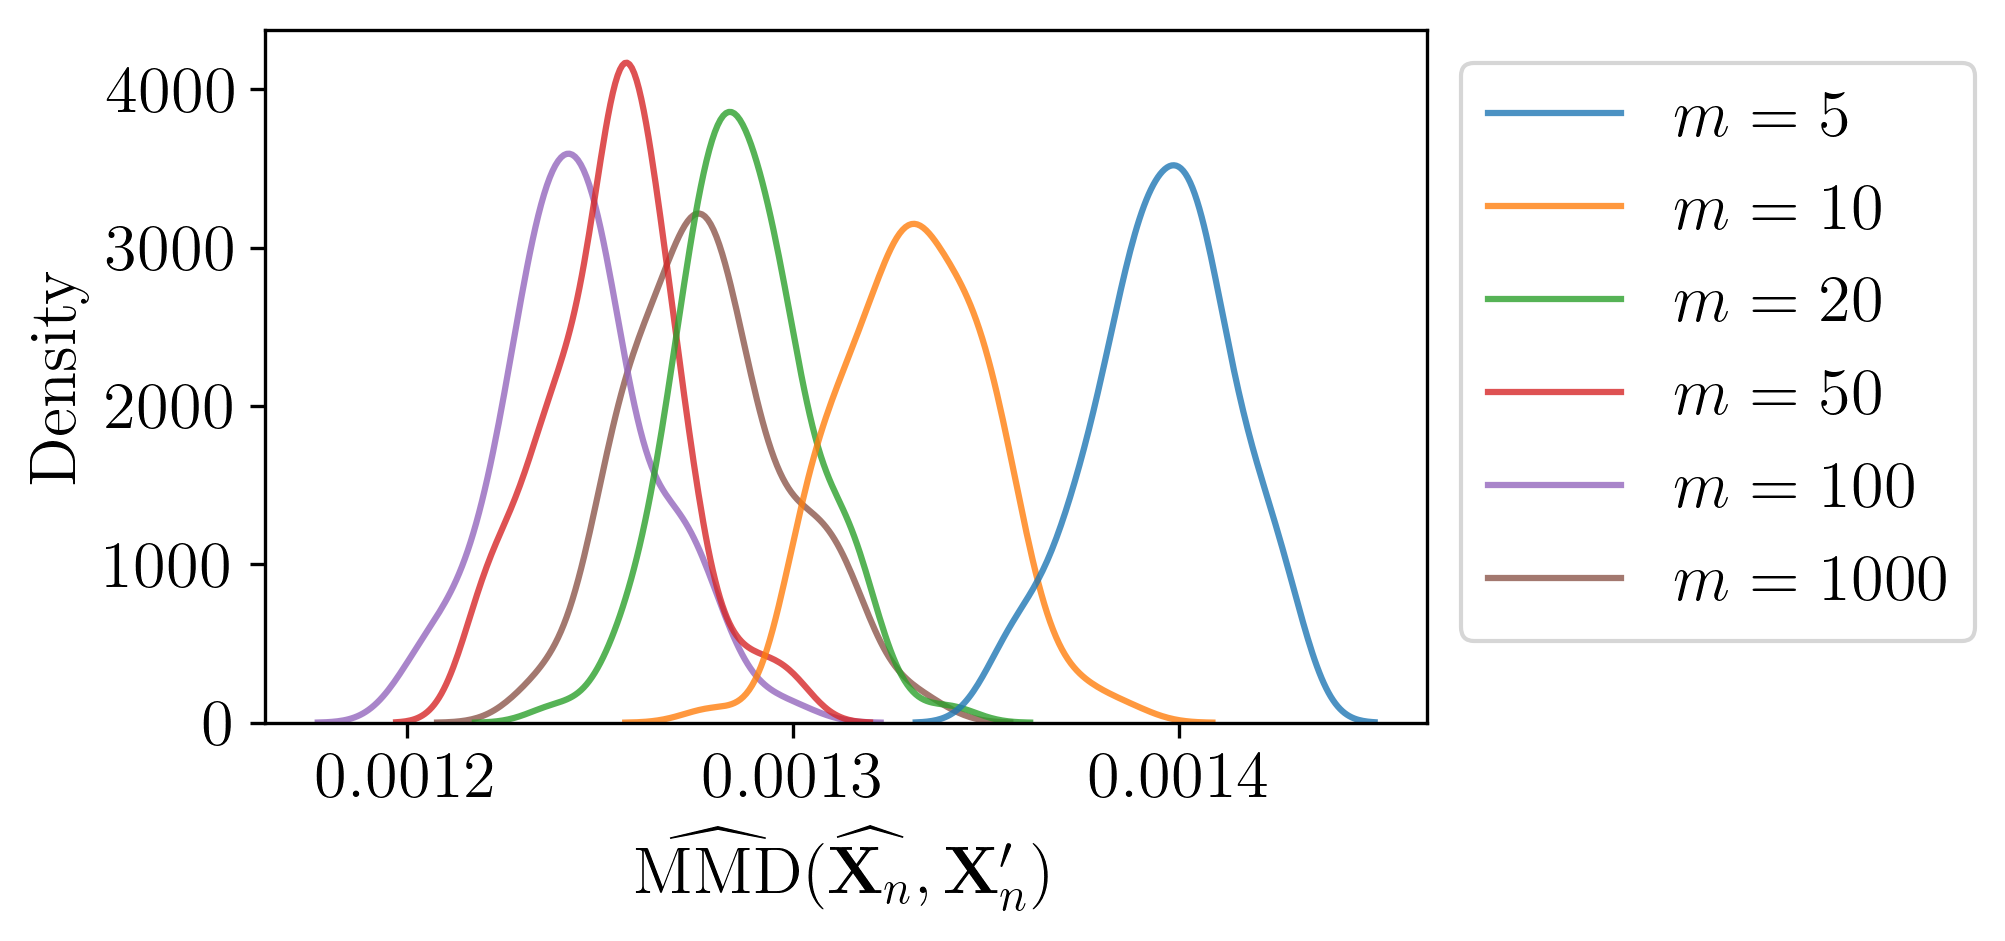
\includegraphics[width=0.7\textwidth]{../numerical_experiments/chapter3/figures/SB_MMD_goodness.png}
    \caption{Empirical distributions of the maximum mean discrepancy between the validation sample $\bX'$ and the sample $\what{\bX_n} \simiid \what{F_\bX}$ (repeated for 100 samples $\what{\bX_n}$).}
    \label{fig:sb_ebc_mmd}
\end{figure}


\begin{landscape}
    \begin{figure}
        \begin{subfigure}[b]{0.49\linewidth}
            \centering
            \includegraphics[width=\linewidth]{../numerical_experiments/chapter3/figures/SB_data_copulogram.png}
            \vspace*{2pt}
            \caption{South Brittany ANEMOC data (size $n=5000$).}
        \end{subfigure}
        \begin{subfigure}[b]{0.49\linewidth}
            \centering
            \includegraphics[width=\linewidth]{../numerical_experiments/chapter3/figures/SB_EBC_copulogram.png}
            \caption{Monte Carlo sample (size $n=5000$), generated from the semiparametric model fitted on the ANEMOC data (EBC $B_{\bm}(C_n)$ with $ \{m_j=100\}_{j=1}^d$).}
        \end{subfigure}
        \vspace*{5pt} 
        \caption{Copulogram of the South Brittany metocean data.}
        \label{fig:sb_copulograms}
    \end{figure}
\end{landscape}




%============================================================%
\subsection{Summary and discussion}
%============================================================%

In this section, a semiparametric inference strategy was illustrated on a metocean dataset from a site off the coast of South Brittany, France. 
This approach is pragmatic and offers a lot of flexibility. 
In our case, the unimodal marginals are fitted by MLE while the multimodal ones are fitted by KDE. 
Considering the complexity of the dependence, the EBC showed interesting results for large-size samples. 
Its capacity to extrapolate in the tails could be further studied \citep{heredia_2022_nonparam_copula} but this tool is an appropriate solution for general inference (for example needed for fatigue assessment). 

In the monograph of \citet{joe2011dependence}, the use of nonparametric methods is briefly discussed p.250. 
The author recommends using nonparametric copulas when the marginals are well-behaved, but the dependence structure is nonlinear. 


%============================================================%
%============================================================%
\section{Quantifying and clustering the wake-induced perturbations within a wind farm}
%============================================================%
%============================================================%

After defining a probabilistic model based on ambient metocean data, the present section studies the impact of the wake on the wind conditions within a farm. 
The wake arises from extracting kinetic energy from the wind, leading to a decrease in wind speed and an increase in turbulence downstream of the turbines. 
In a wind farm, the wake mostly depends on the turbines' layout, the ambient wind speed, and the ambient turbulence intensity. 
The resulting heterogeneous wind field in a wind farm can be simulated by numerical models with different fidelities (as discussed in Section~\ref{sec:222}). 

In our case, simplified wake models (sometimes called ``dynamic wake meandering'', or ``engineering'' models, see e.g., \citealp{doubrawa_2020_benchmark}) are used to simulate the wind speed deficit and the added turbulence at each turbine.
To recover a wake-perturbed wind distribution at each turbine, the ambient wind distribution is propagated through a wake model. 
Having different wind distributions naturally impacts the loading and should be considered during fatigue assessment at a farm scale. 
Such heterogeneity is mostly considered by international standards via empirical coefficients (also called ``effective turbulence''). 
\citet{doubrawa_2023} compares the effective turbulence approach with dynamic wake meandering models and studies their impact on loading. 

In practice, fatigue assessment on a turbine represents a computational effort. 
As a consequence of wake modeling, each turbine presents a different wind distribution, which implies repeating a fatigue assessment for every turbine. 
To make this computation tractable at a farm scale, the present section aims at building clusters of turbines similarly affected by the wake. 
Then, fatigue assessment can be computed on a few turbines, each representing a cluster of turbines facing similar wake-modified wind loading. 
The maximum mean discrepancy (MMD) is used as a statistical dissimilarity measure to compare the perturbed distributions induced by the wake. 

This new approach is applied to a theoretical wind farm representing the recent call for tenders off the coast of South Brittany, France. 
The turbines considered are a modified version of the floating offshore wind turbine (FOWT) IEA-15MW (described in \citealp{kim_natarajan_2022}). 
Figure~\ref{fig:SB-farm} illustrates the layout of the 25 FOWTs modeled in the following, the coordinates are normalized by the rotor's diameter $D$. 
The spacing between turbines in this regular layout is equivalent to seven rotor diameters in the dominant wind direction and five rotor diameters in the orthogonal direction (i.e., crosswind). 

To develop this approach on the South Brittany farm, the present section is structured as follows: 
first, the wake model and its corresponding uncertainty propagation are presented, 
then MMDs are estimated between the resulting empirical joint wind distributions, 
and finally, a simple clustering gathers turbines perceiving similar wakes and defines their representative turbines. 
In the end, the 25 FOWT are split into four groups, whose representatives can be used for the fatigue assessment of the whole group. 

\begin{figure}
    \centering
    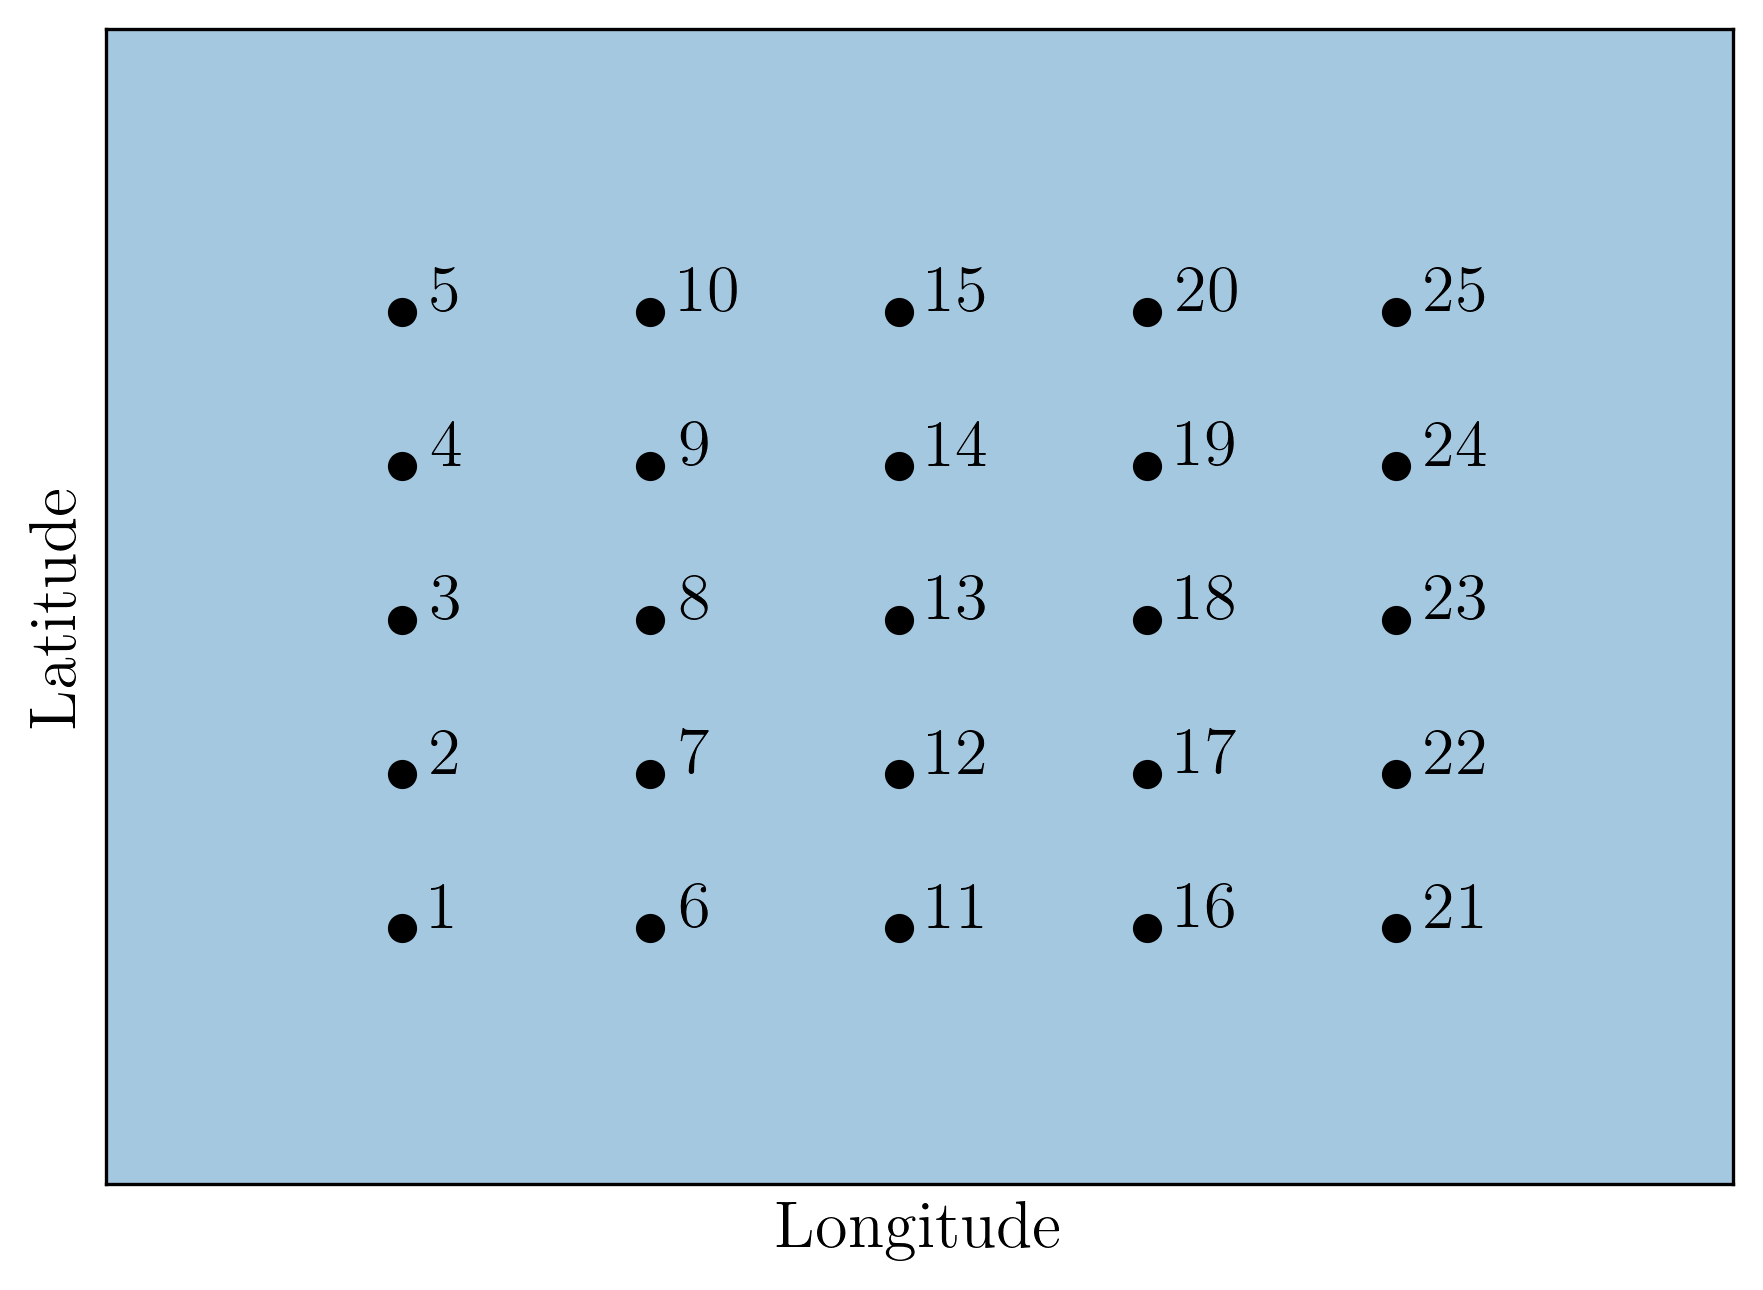
\includegraphics[width=0.48\textwidth]{part2/figures/WAKE/layout_SB.png}
    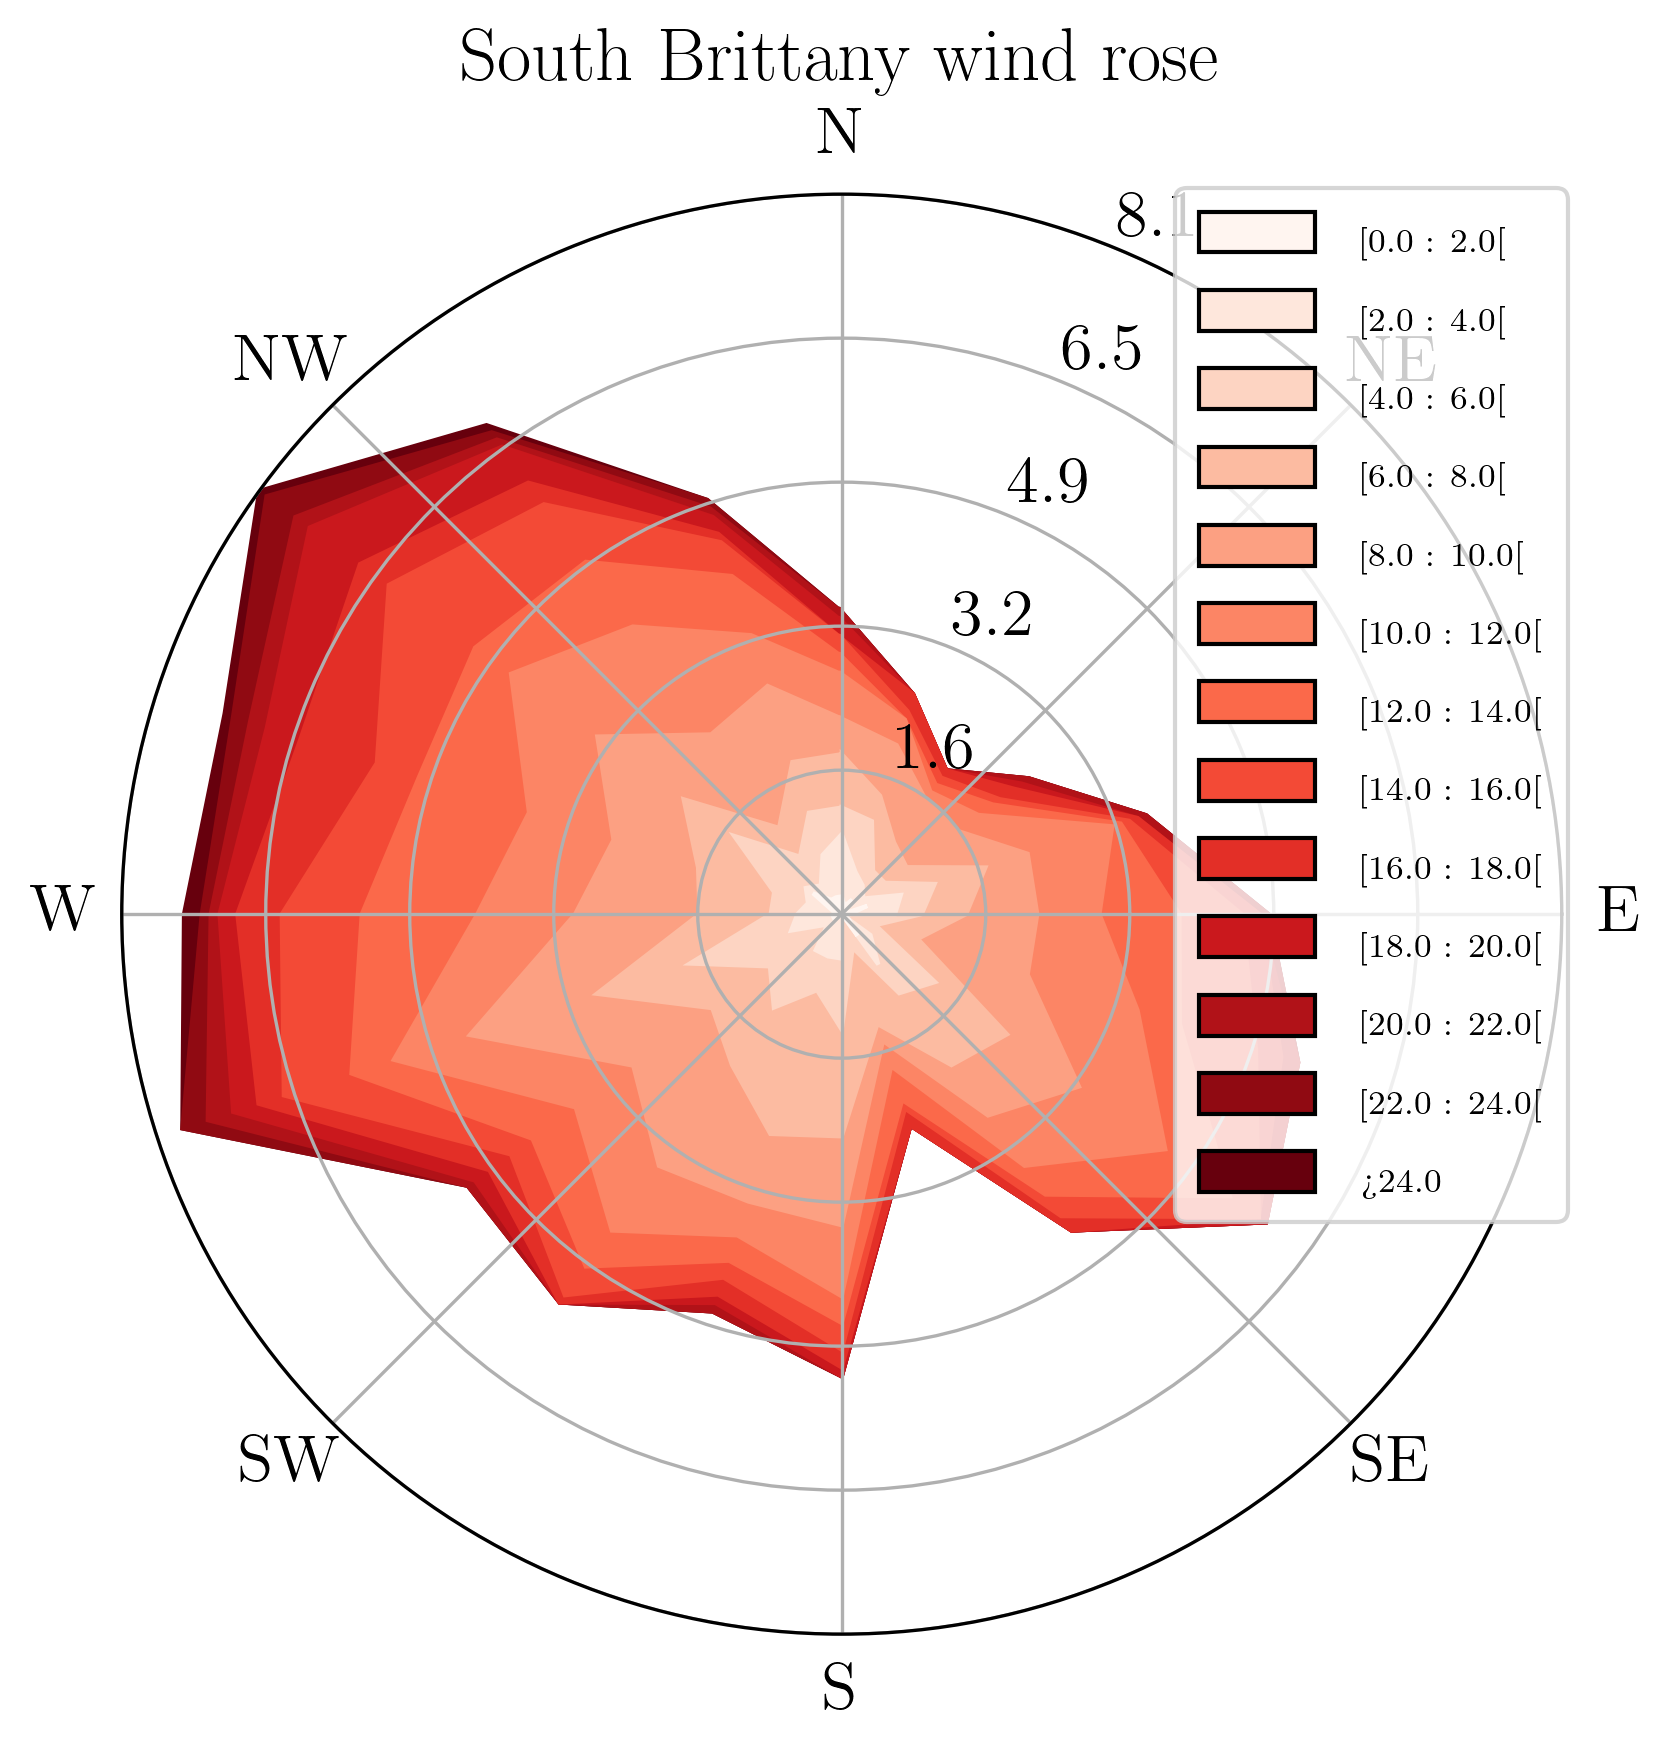
\includegraphics[width=0.4\textwidth]{../numerical_experiments/chapter3/figures/SB_wind_rose.png}
    \caption{South Brittany wind farm layout, the vertical direction does not represent the exact north (left). South Brittany wind rose from the ANEMOC data (right).}
    \label{fig:SB-farm}
\end{figure}


%============================================================%
\subsection{Uncertainty propagation on a wake model}\label{sec:UQ-wake}
%============================================================%

%------------------------------------------------------------%
\paragraph{Wake model definition}
%------------------------------------------------------------%
When simulating the wake effect of floating wind turbines, different studies (either using dynamic wake meandering \cite{wise_2020} or LES \cite{johlas_2020_wake_LES}), showed the importance of modeling the floaters' position (translation and rotation). 
Therefore, an engineering wake model based on the Farmshadow™ software (developed by IFPEN) was coupled with a hydro-static calculation to predict the floater's position, as well as the wind speed and turbulence intensity. 
In this model, the floaters are considered to be rigid, and all degrees of freedom are considered (surge, sway and heave for the three translations and roll, pitch and yaw for the three rotations). 

FarmShadow™ uses engineering wake models to simulate the wind field throughout the whole farm, starting from the most upstream WT and working downwards. 
More precisely, the model used includes the ``super-gaussian'' approach for speed deficit \citep{blondel_2020}, waked-induced turbulence according to \citet{quian_2018}, and superimposition following the linear sum approach defined by \citet{zong_2020}.    
Further assumptions regarding the hydro-statics loading, the effect of the mooring lines, and the wake model are defined in \citet{lovera_fekhari_2023}.


%------------------------------------------------------------%
\paragraph{Monte Carlo uncertainty propagation}
%------------------------------------------------------------%

The wake model described earlier takes as input a set of variables describing the ambient wind conditions $\bx \in \mathbb{R}^3$ and computes the perturbed wind conditions at each WT represented by the vector $\bx _l', l \in (1,..,n_{WT})$, where $n_{WT} \in \N$ is the total number of turbines in the farm:
\begin{align}
    g:\mathbb{R}^3 &\rightarrow \mathbb{R}^{3 n_{WT}} \\
    \bx &\longmapsto g(\bx) = (\bx_1',..,\bx_{n_{WT}}')
\end{align}
The uncertainties associated with the ambient wind conditions are represented by a random vector $\bX$ following the distribution $f_0$. 
A parametric model has been fitted in \cite{vanem_fekhari_2023} using conditional probability density functions to capture the dependence structure, 
but the semi-parametric inference proposed in Section~\ref{sec:32_inference} could have been an alternative. 
Note that the missing turbulence intensity in the ANEMOC data from South Brittany was assumed to follow a lognormal distribution.   
The random vector $\bX$ gathers the following random variables:
\begin{itemize}
    \item Mean wind speed ($U$) is the 10-min average horizontal wind speed at hub height.
    \item Wind turbulence intensity ($TI$) is the 10-min wind speed turbulence intensity at hub height.
    \item Wind direction ($\theta_{\mathrm{wind}}$) is the 10-min average wind direction.
\end{itemize}

In the following, the wind orientation $\theta_{\mathrm{wind}}$ is supposed to be unaffected by the wake. 
The uncertainty propagation through the wake models provides a set of perturbed environmental distributions $f_l', l \in (1,..,n_{WT})$. 
In practice, a Monte Carlo sample $\bX_n={\bx^{(1)},..,\bx^{(n)}} \sim \bX$ (with size n=6000) is generated and evaluated by the wake model. 
Since the model has a low computational cost, Monte Carlo sampling was affordable while giving strong convergence guarantees. 

\fig{fig:FIGJointPerturbationSB} illustrates the perturbation of the wind distributions for three WT differently affected by the wake depending on their position in the farm (see Figure~\ref{fig:SB-farm}). 
One can notice that the distribution of WT~25 (in orange) is very close to the ambient distribution (in black), as expected since this WT is located on the edge of the farm and facing the dominant wind direction. 
Meanwhile, the distribution of WT~13 (in red) seems more affected by the wake, by getting higher wind turbulence with lower wind speed. 
This analysis can be completed with the two marginals in \fig{fig:FIGMarginalWSP} and \fig{fig:FIGMarginalTI}, both describing the ambient marginal distributions (in black) and wake-disturbed distributions. 
In general, a small wind speed deficit is indicated by the small shifts of the probability density functions to the left on \fig{fig:FIGMarginalWSP}. 
Also, a small added turbulence is noticeable with shifts of the PDFs to the right on \fig{fig:FIGMarginalTI}. 
A tool is needed to quantify the wind perturbations induced by the wake.

\begin{figure}
    \centering
    \begin{subfigure}[b]{0.48\textwidth}
        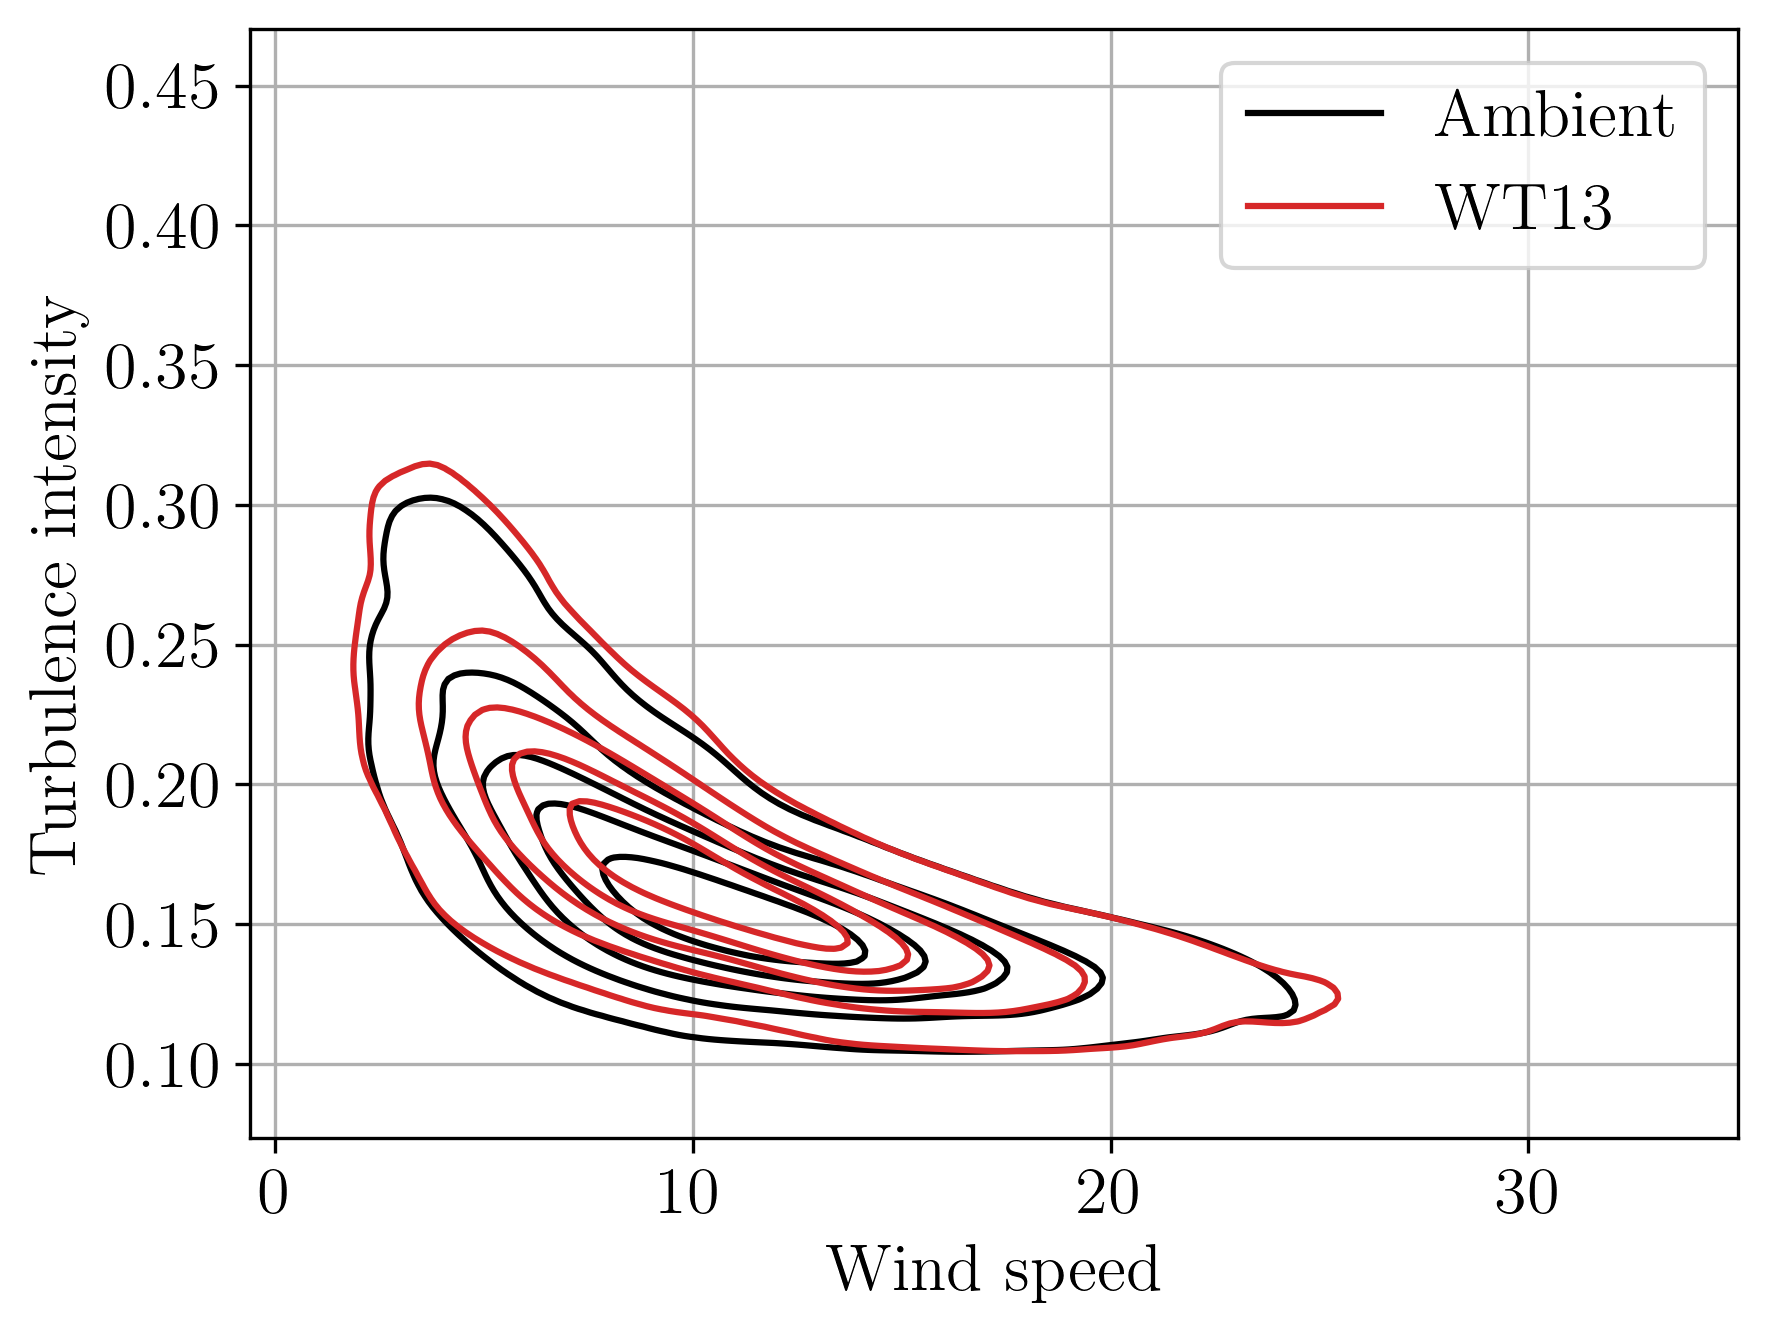
\includegraphics[width=\textwidth]{part2/figures/WAKE/joint_perturbation_SB_WT13.png}
    \end{subfigure}
    \begin{subfigure}[b]{0.48\textwidth}
        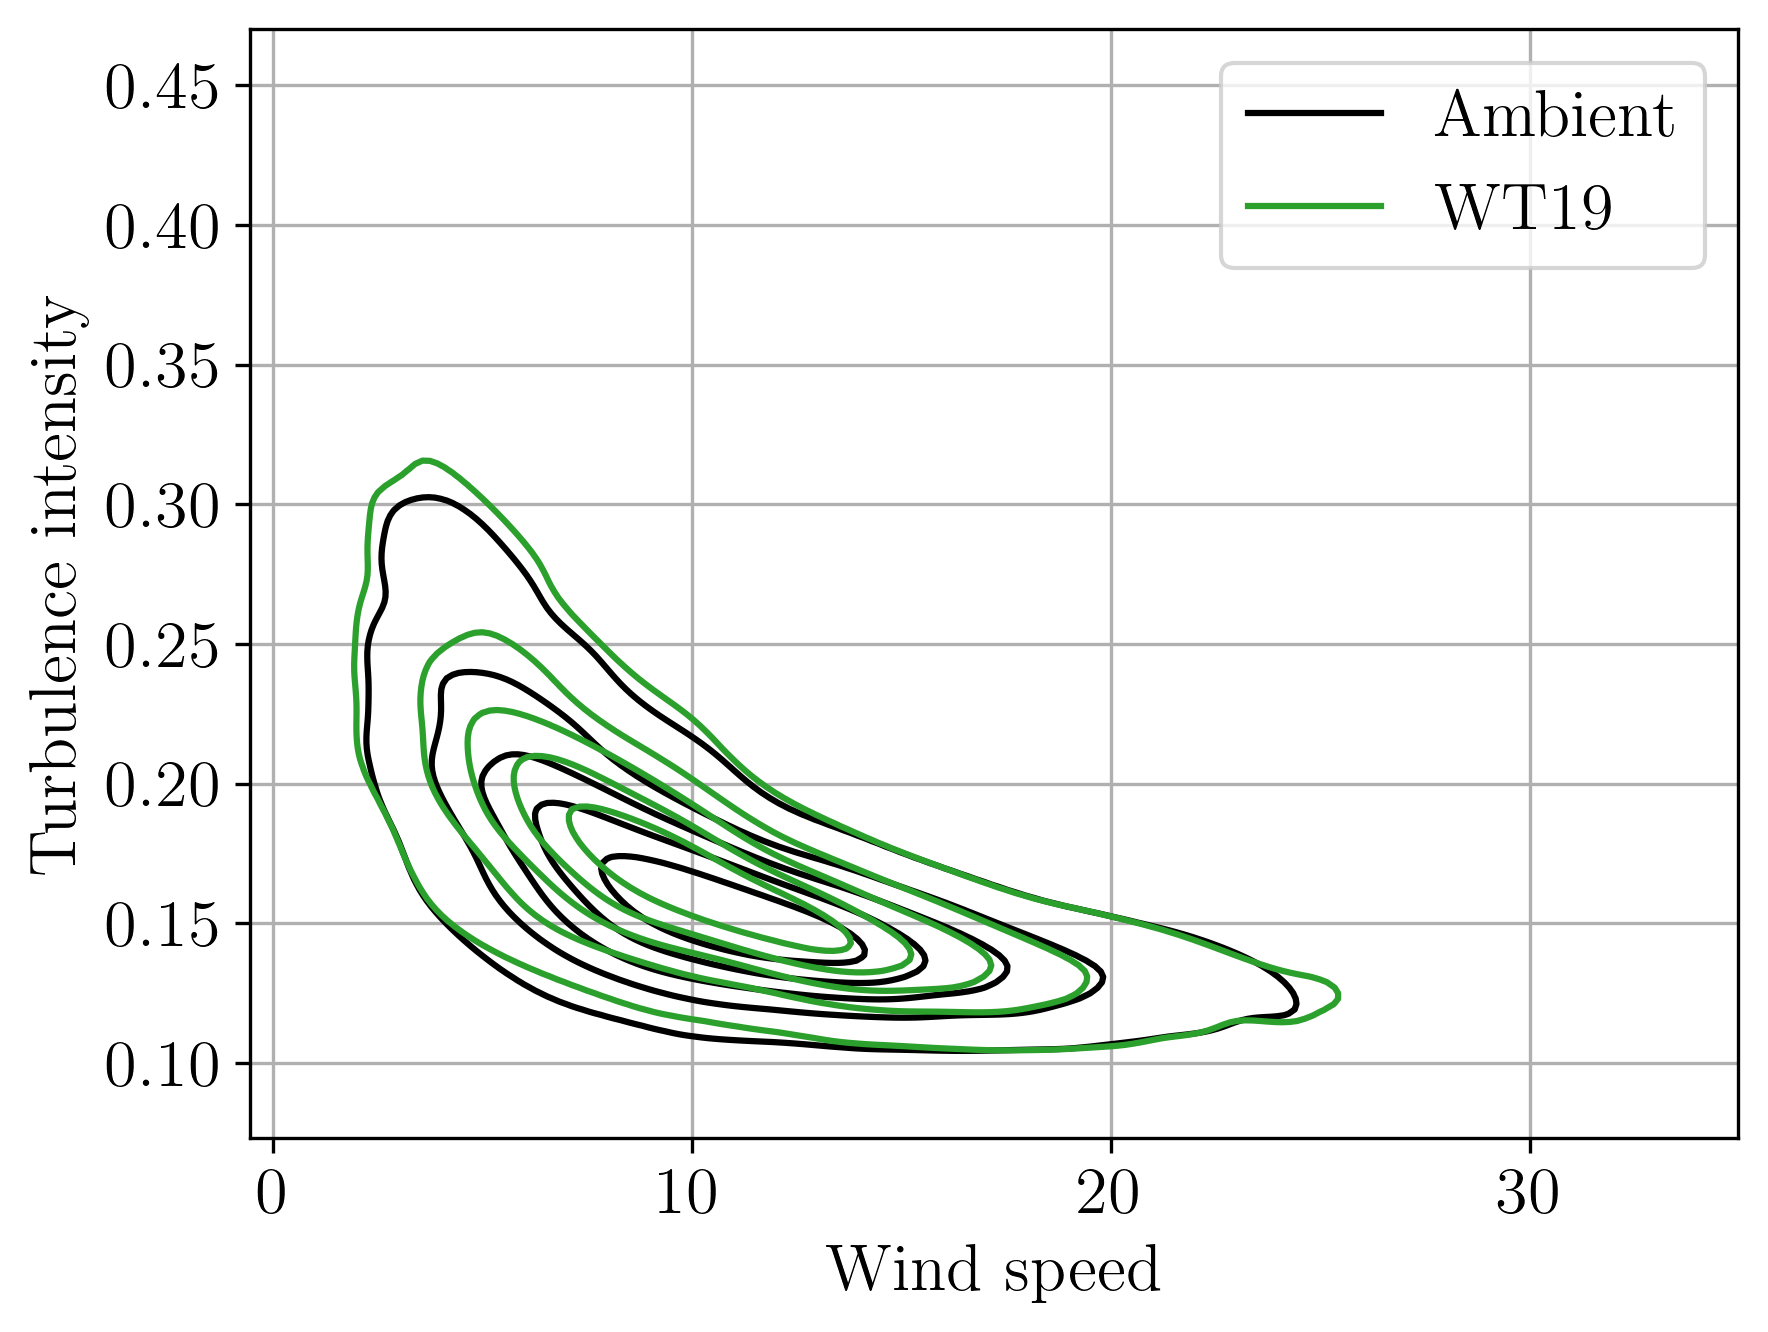
\includegraphics[width=\textwidth]{part2/figures/WAKE/joint_perturbation_SB_WT19.png}
    \end{subfigure}
    \\
    \begin{subfigure}[b]{0.48\textwidth}
        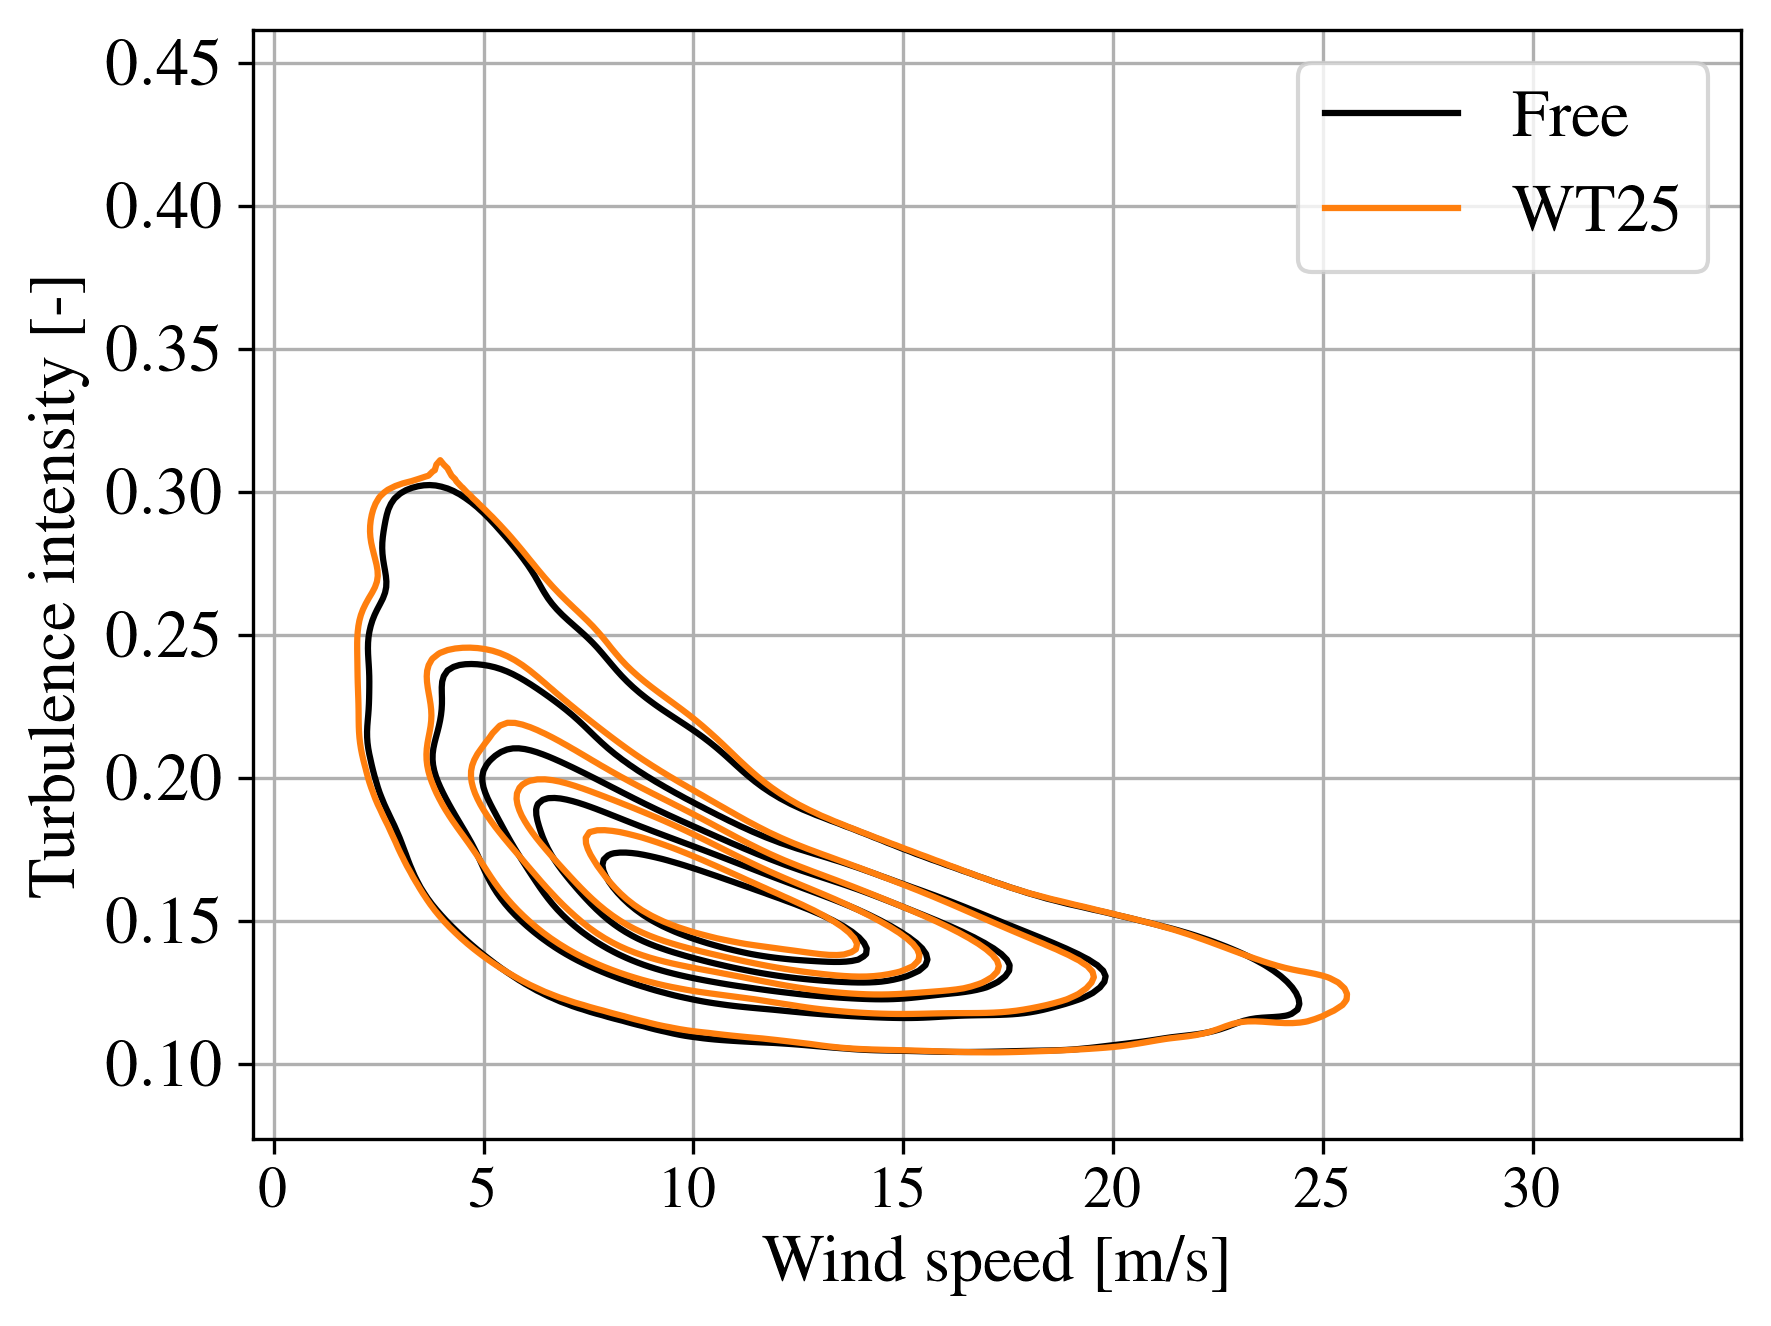
\includegraphics[width=\textwidth]{part2/figures/WAKE/joint_perturbation_SB_WT25.png}
    \end{subfigure}
    \caption{Joint distributions of the wake-perturbed wind conditions at WT 13, 19, and 25 (in color) compared with the ambient wind conditions (in black).}
    \label{fig:FIGJointPerturbationSB}
\end{figure}

\begin{figure}
    \centering
    \begin{subfigure}[b]{0.48\textwidth}
        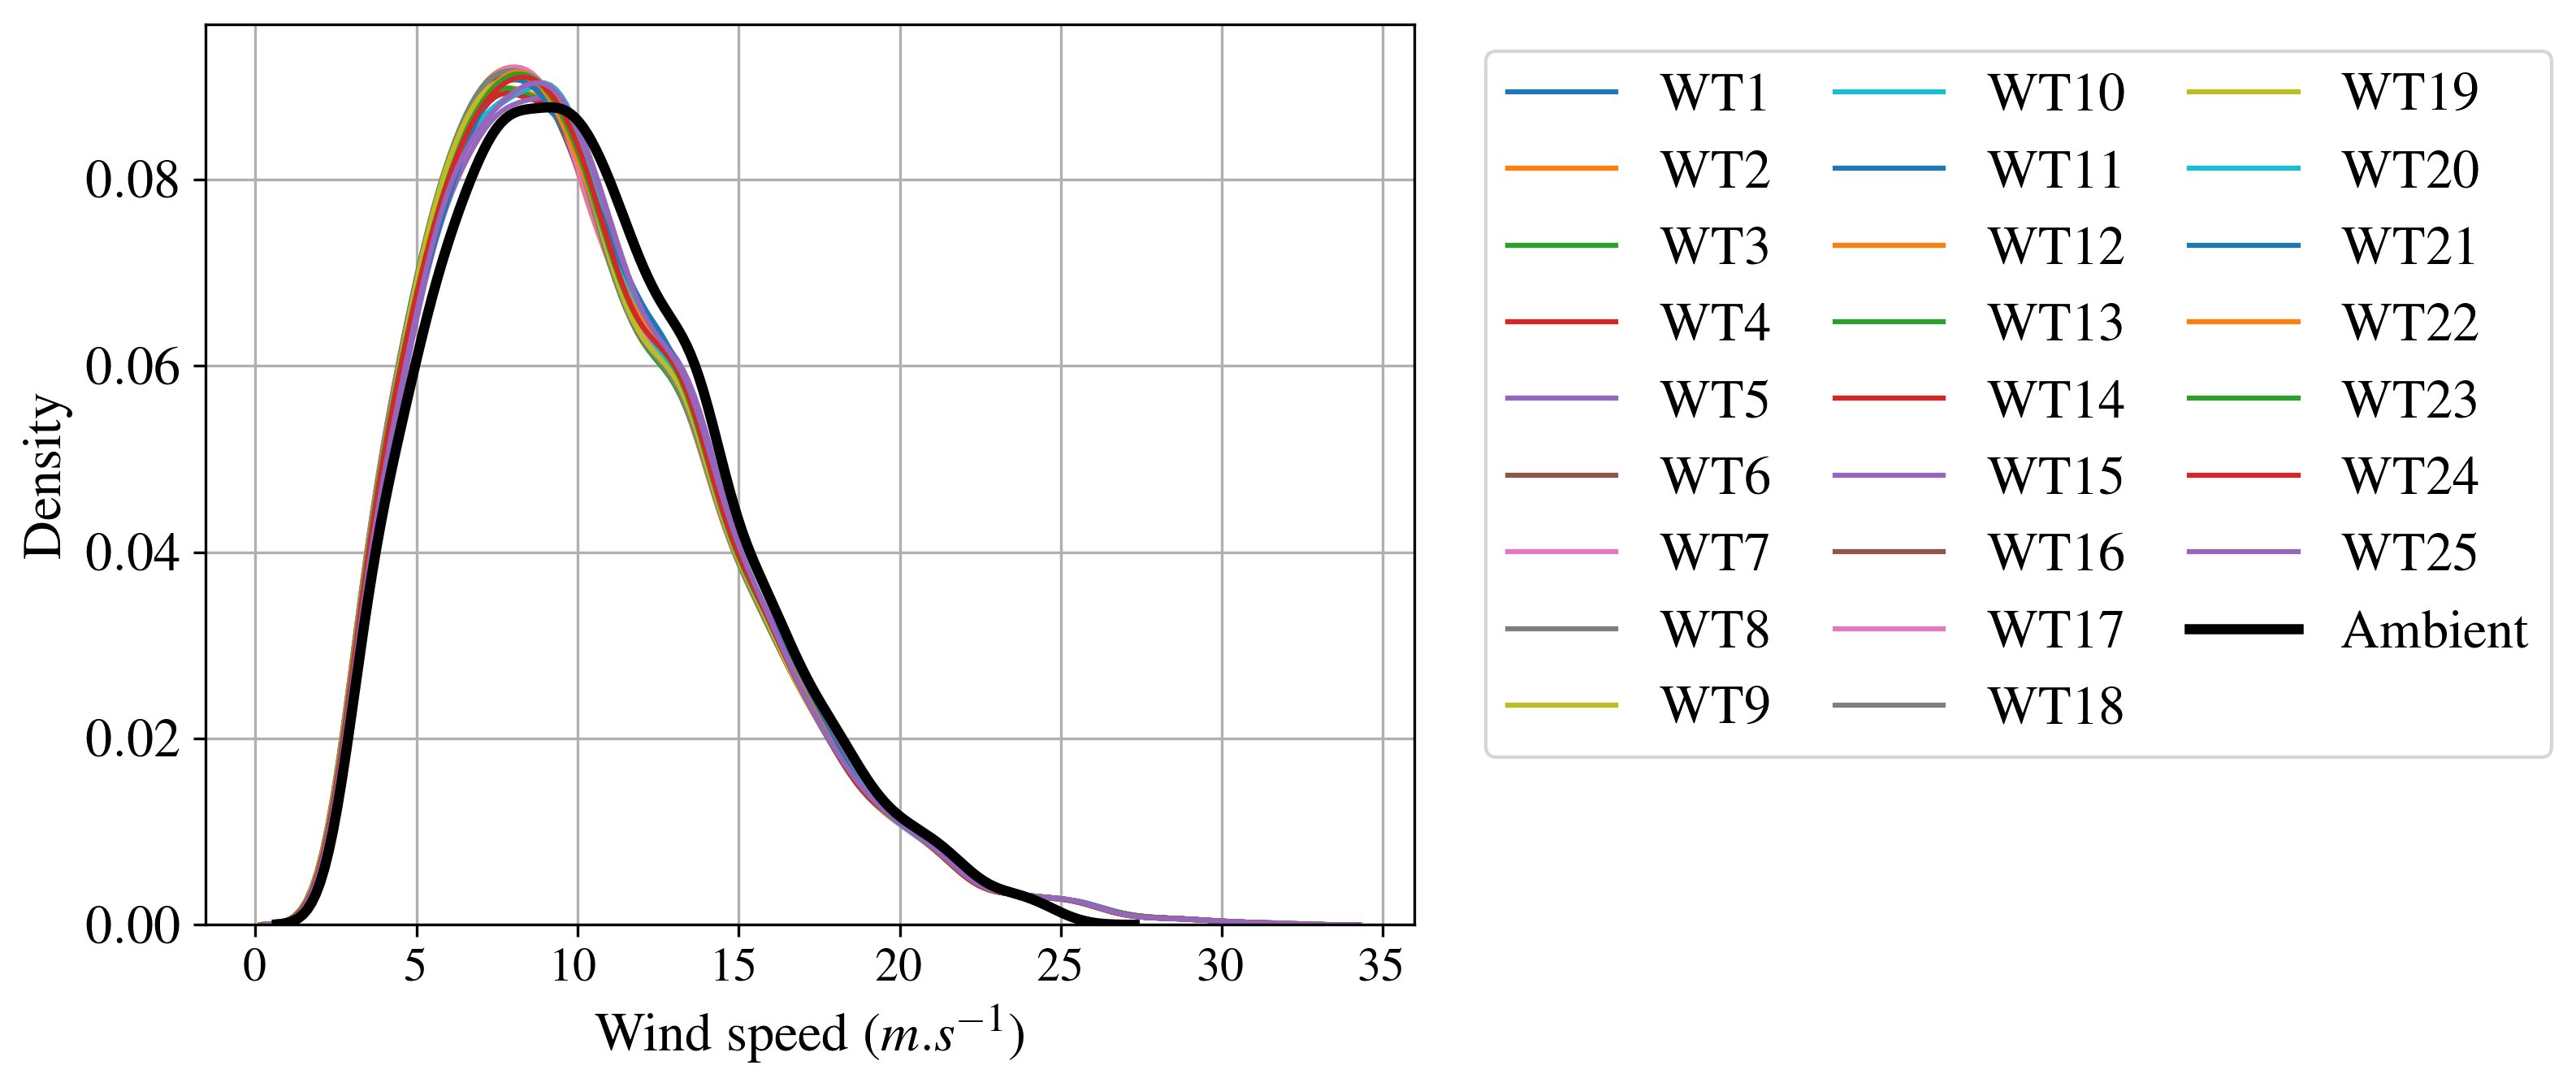
\includegraphics[width=\textwidth]{part2/figures/WAKE/perturbed_wsp_distribution_SB.png}
        \caption{Wind speed.}
        \label{fig:FIGMarginalWSP}
    \end{subfigure}
    \begin{subfigure}[b]{0.48\textwidth}
        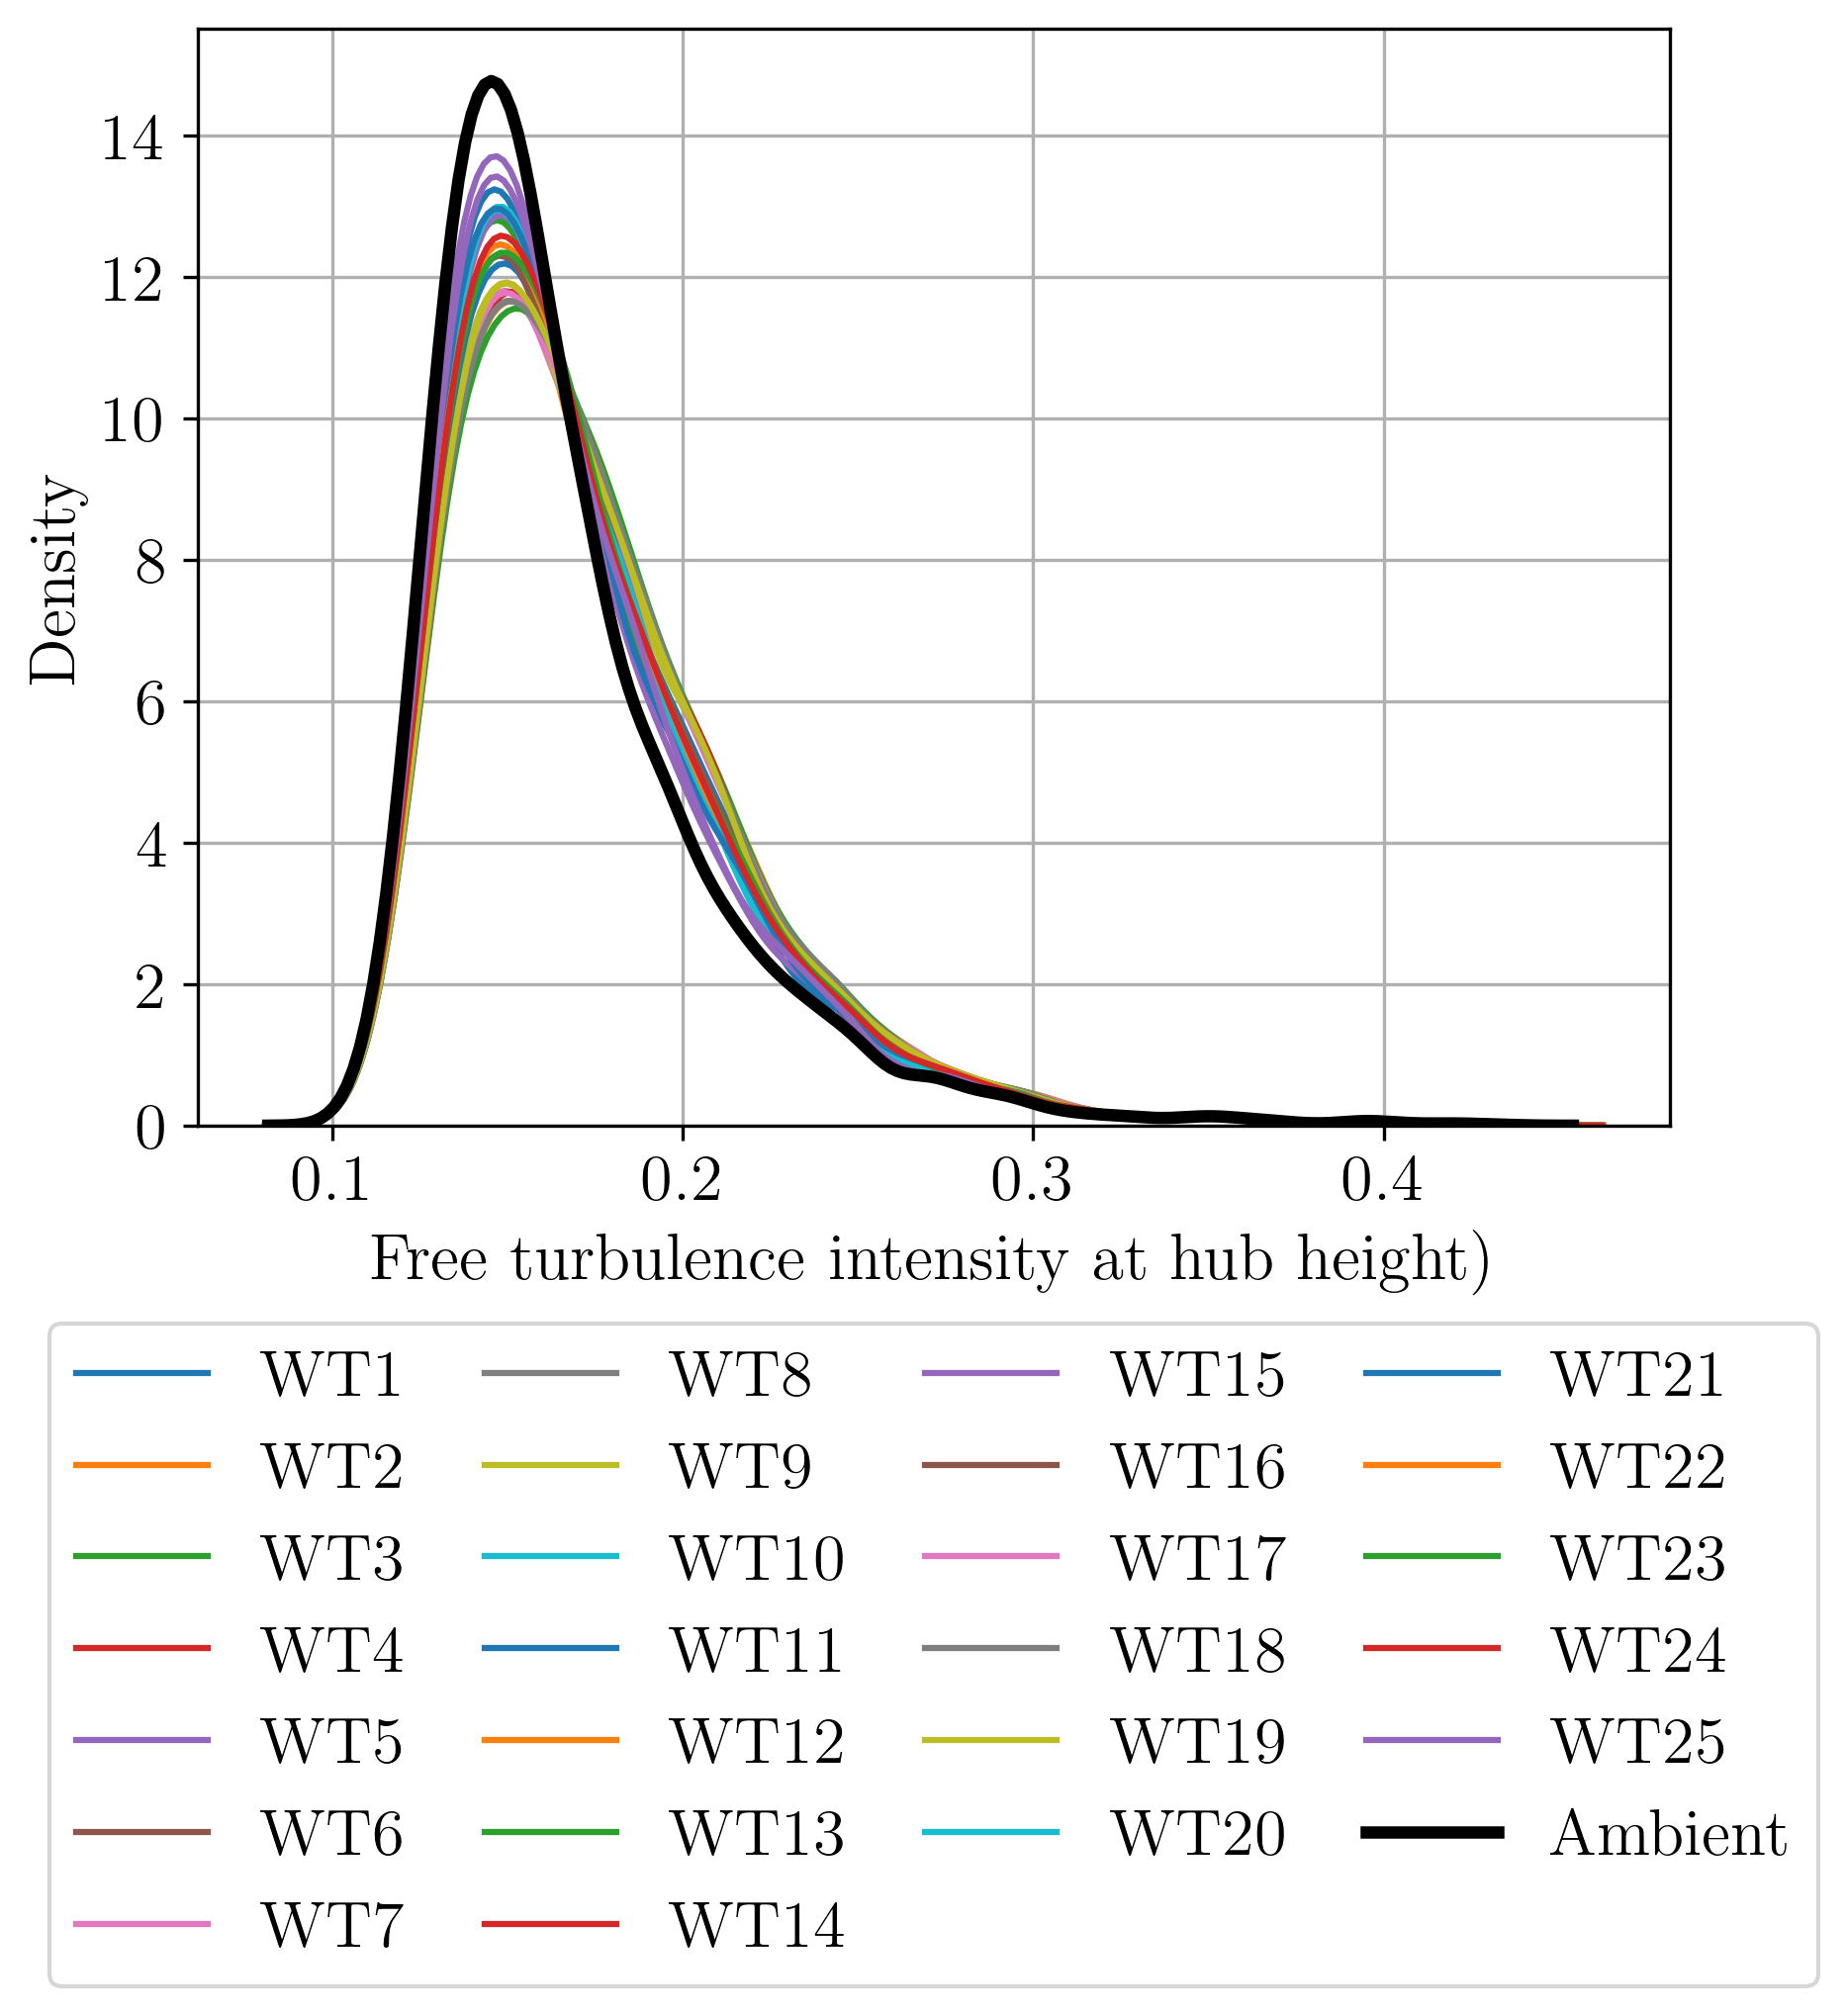
\includegraphics[width=\textwidth]{part2/figures/WAKE/perturbed_ti_distribution_SB.png}
        \caption{Turbulence intensity.}
        \label{fig:FIGMarginalTI}
    \end{subfigure}
    \caption{Ambient (in black) and wake-perturbed (in color) distributions of wind distributions.}
\end{figure}





%============================================================%
\subsection{Statistical metric of wake-induced perturbations}\label{sec:metric}
%============================================================%


The maximum mean discrepancy was introduced by \cite{gretton_2006} as a statistic for two-sample testing. 
After further work on this tool, authors such as \cite{sriperumbudur_2010} showed that the MMD is a distance between two distributions embedded in a specific function space. 
The MMD becomes a metric for specific kernels called “characteristic kernels”, which offer the following property: $\MMD(\pi, \zeta)=0 \iff \pi = \zeta$. 
The squared MMD has been used for multiple purposes and is further presented in Appendix~\ref{apx:B}
In the following, the idea is to compare the ambient wind distribution $f_0$ to the wake-perturbed wind conditions $f_l'$ at the WT~$l$ using the squared MMD.

%------------------------------------------------------------%
\paragraph{Application to the South Brittany wind farm project}
%------------------------------------------------------------%
Once the joint perturbed distributions of each WT are evaluated on a large Monte Carlo sample, their squared MMD with the ambient wind conditions can be computed. 
\fig{fig:FIGWakeEffect} represents the squared MMD for each WT to quantify the wake-induced perturbation. 
The values of squared MMD presented in this figure are estimated between two Monte Carlo samples with size $n=6000$. 
A verification of their convergence is realized in terms of coefficient of variation. 

\begin{figure}
    \centering
    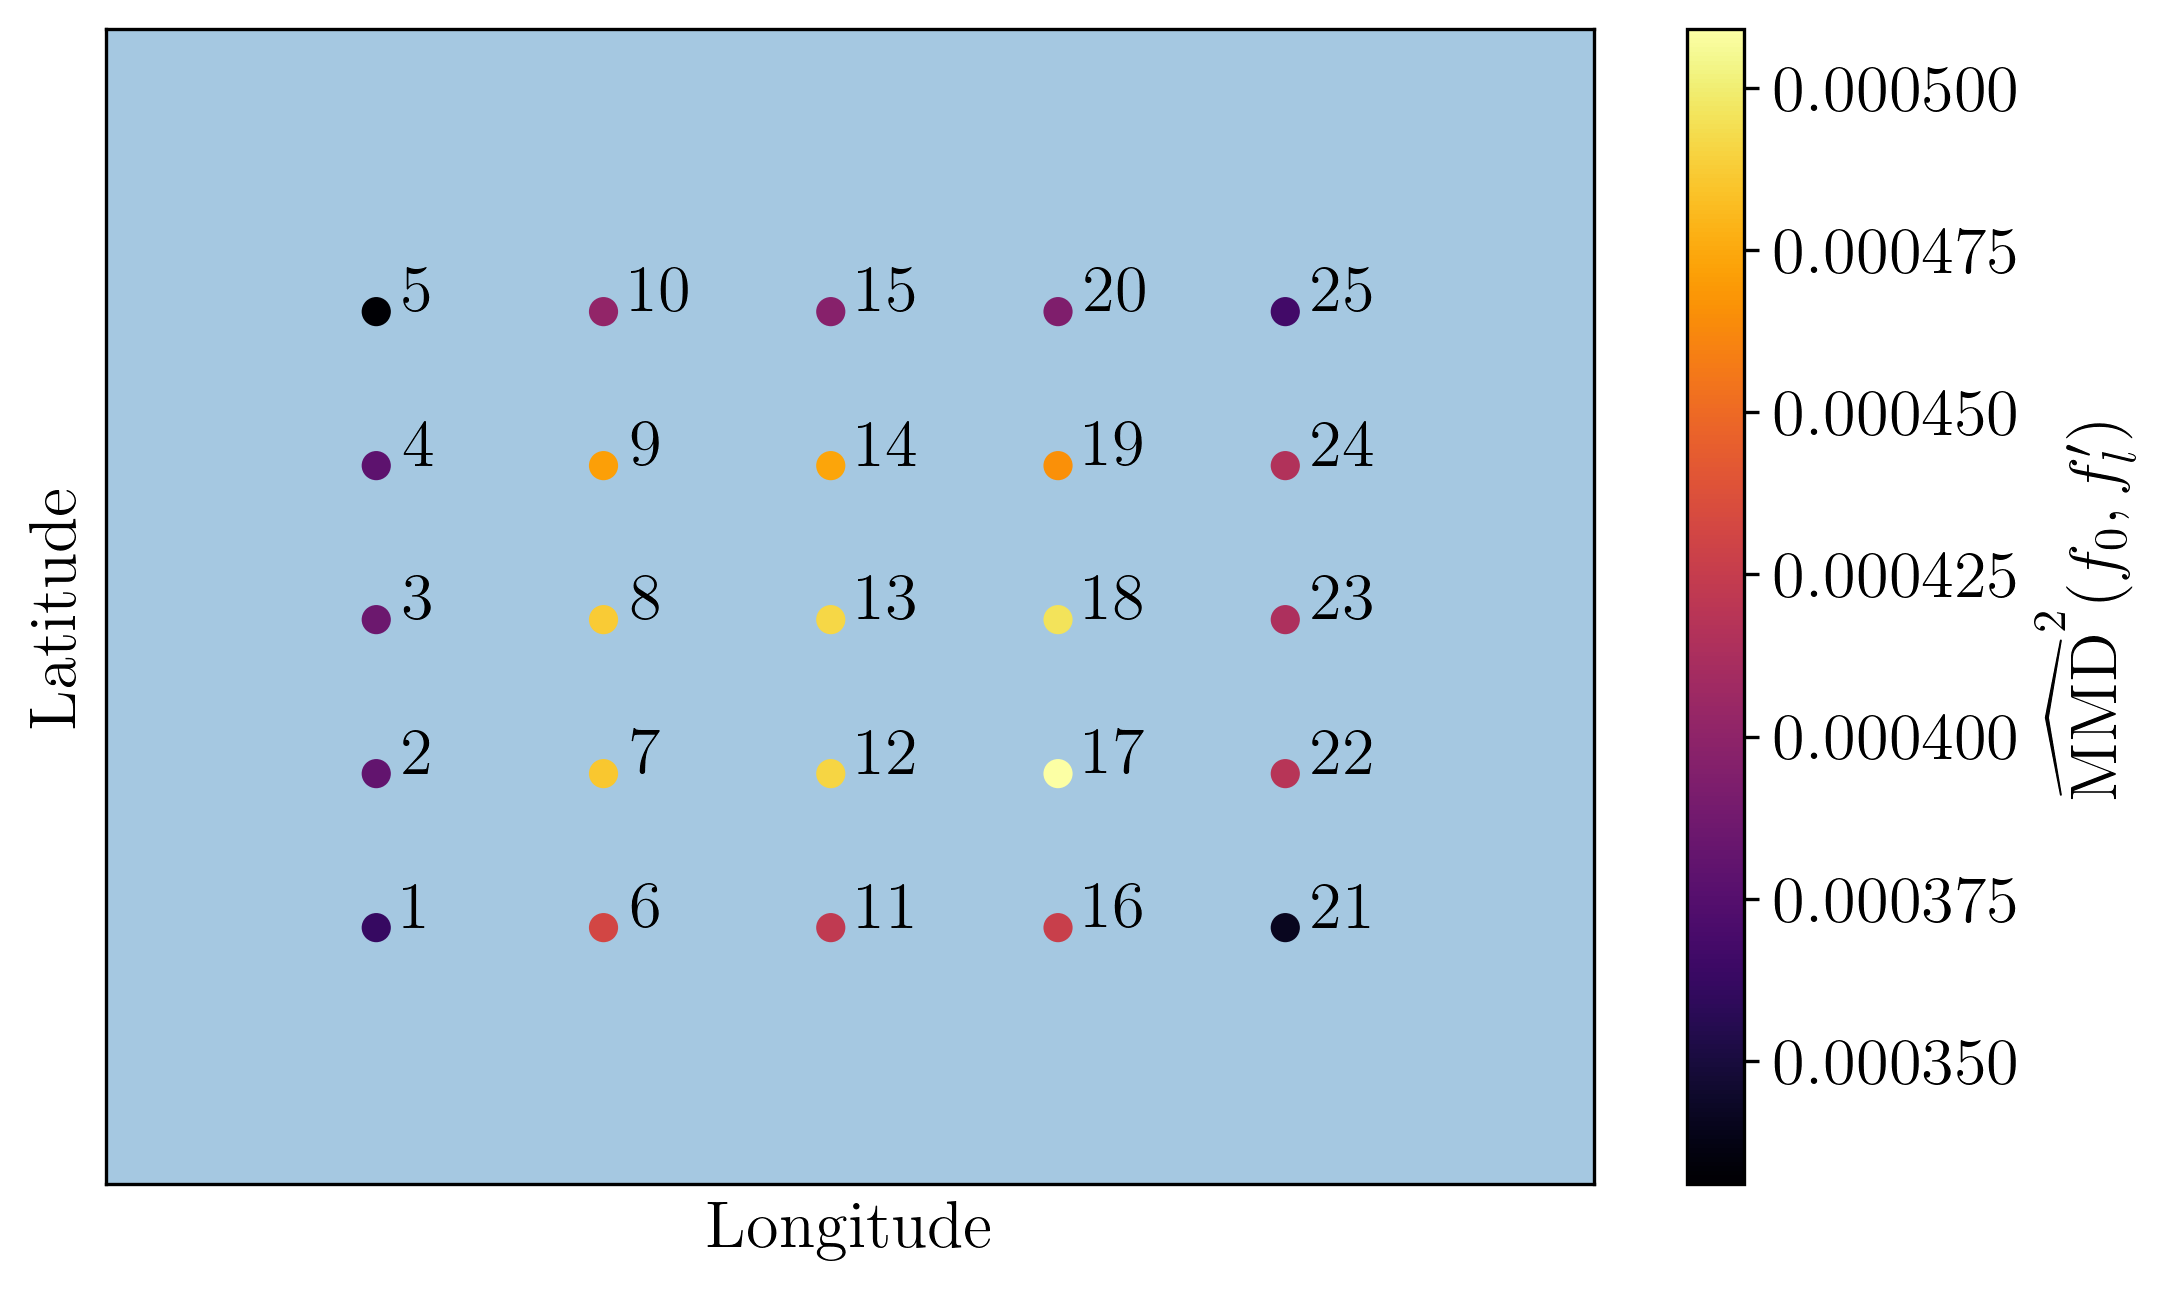
\includegraphics[width=0.6\textwidth]{part2/figures/WAKE/wake_perturbation_SB.png}
    \caption{South Brittany layout and wake effects measured by the squared MMD on wind conditions. 
    Note that the vertical direction does not represent the north direction.}
    \label{fig:FIGWakeEffect}
\end{figure}

%============================================================%
\subsection{Clustering the wake-induced perturbations}
%============================================================%

The aim of this section is to use the MMD as a metric to define clusters of turbines getting similar wind conditions. 
Instead of comparing the wake-perturbed distributions with the ambient one, let us compare all the pairs of wake-perturbed distributions. 
Considering all the WT $\{1, \dots, n_{WT}\}$ in the farm, and their respective wake-perturbed distributions $\{f_l'\}_{l=1}^{n_{WT}}$, let us define the symmetric matrix $D$ of MMD between every pair of perturbed distributions such that $D_{i, j} = \what{\mathrm{MMD}}^2(f_i', f_j')$. 

Different unsupervised clustering techniques, such as hierarchical or centroid-based methods were compared in \citet{lovera_fekhari_2023}. 
The ``k-medoids'' \citep{park_2009} are a variation of the well-known k-means that selects actual data points as centers (i.e., medoids). 
In our case, this method not only gathers turbines with the same wind conditions but also determines a representative turbine for each cluster. 

Assuming a final number of clusters equal to five, \fig{fig:kmedoids} represents the clusters defined by the k-medoid method applied to the matrix $D$. 
Let us notice that the results are rather coherent with the main wind orientation illustrated in the wind rose (see \fig{fig:SB-farm}). 
Interestingly, the conclusion that emerged from comparing the wake-perturbed distributions to the ambient one (see \fig{fig:FIGWakeEffect}) is different from the ones obtained by comparing pairs of wake-perturbed distributions. 
Finally, the representative turbines are tagged with the mention ``r'' and could be used to perform a fatigue analysis. 


\begin{figure}
    \centering
    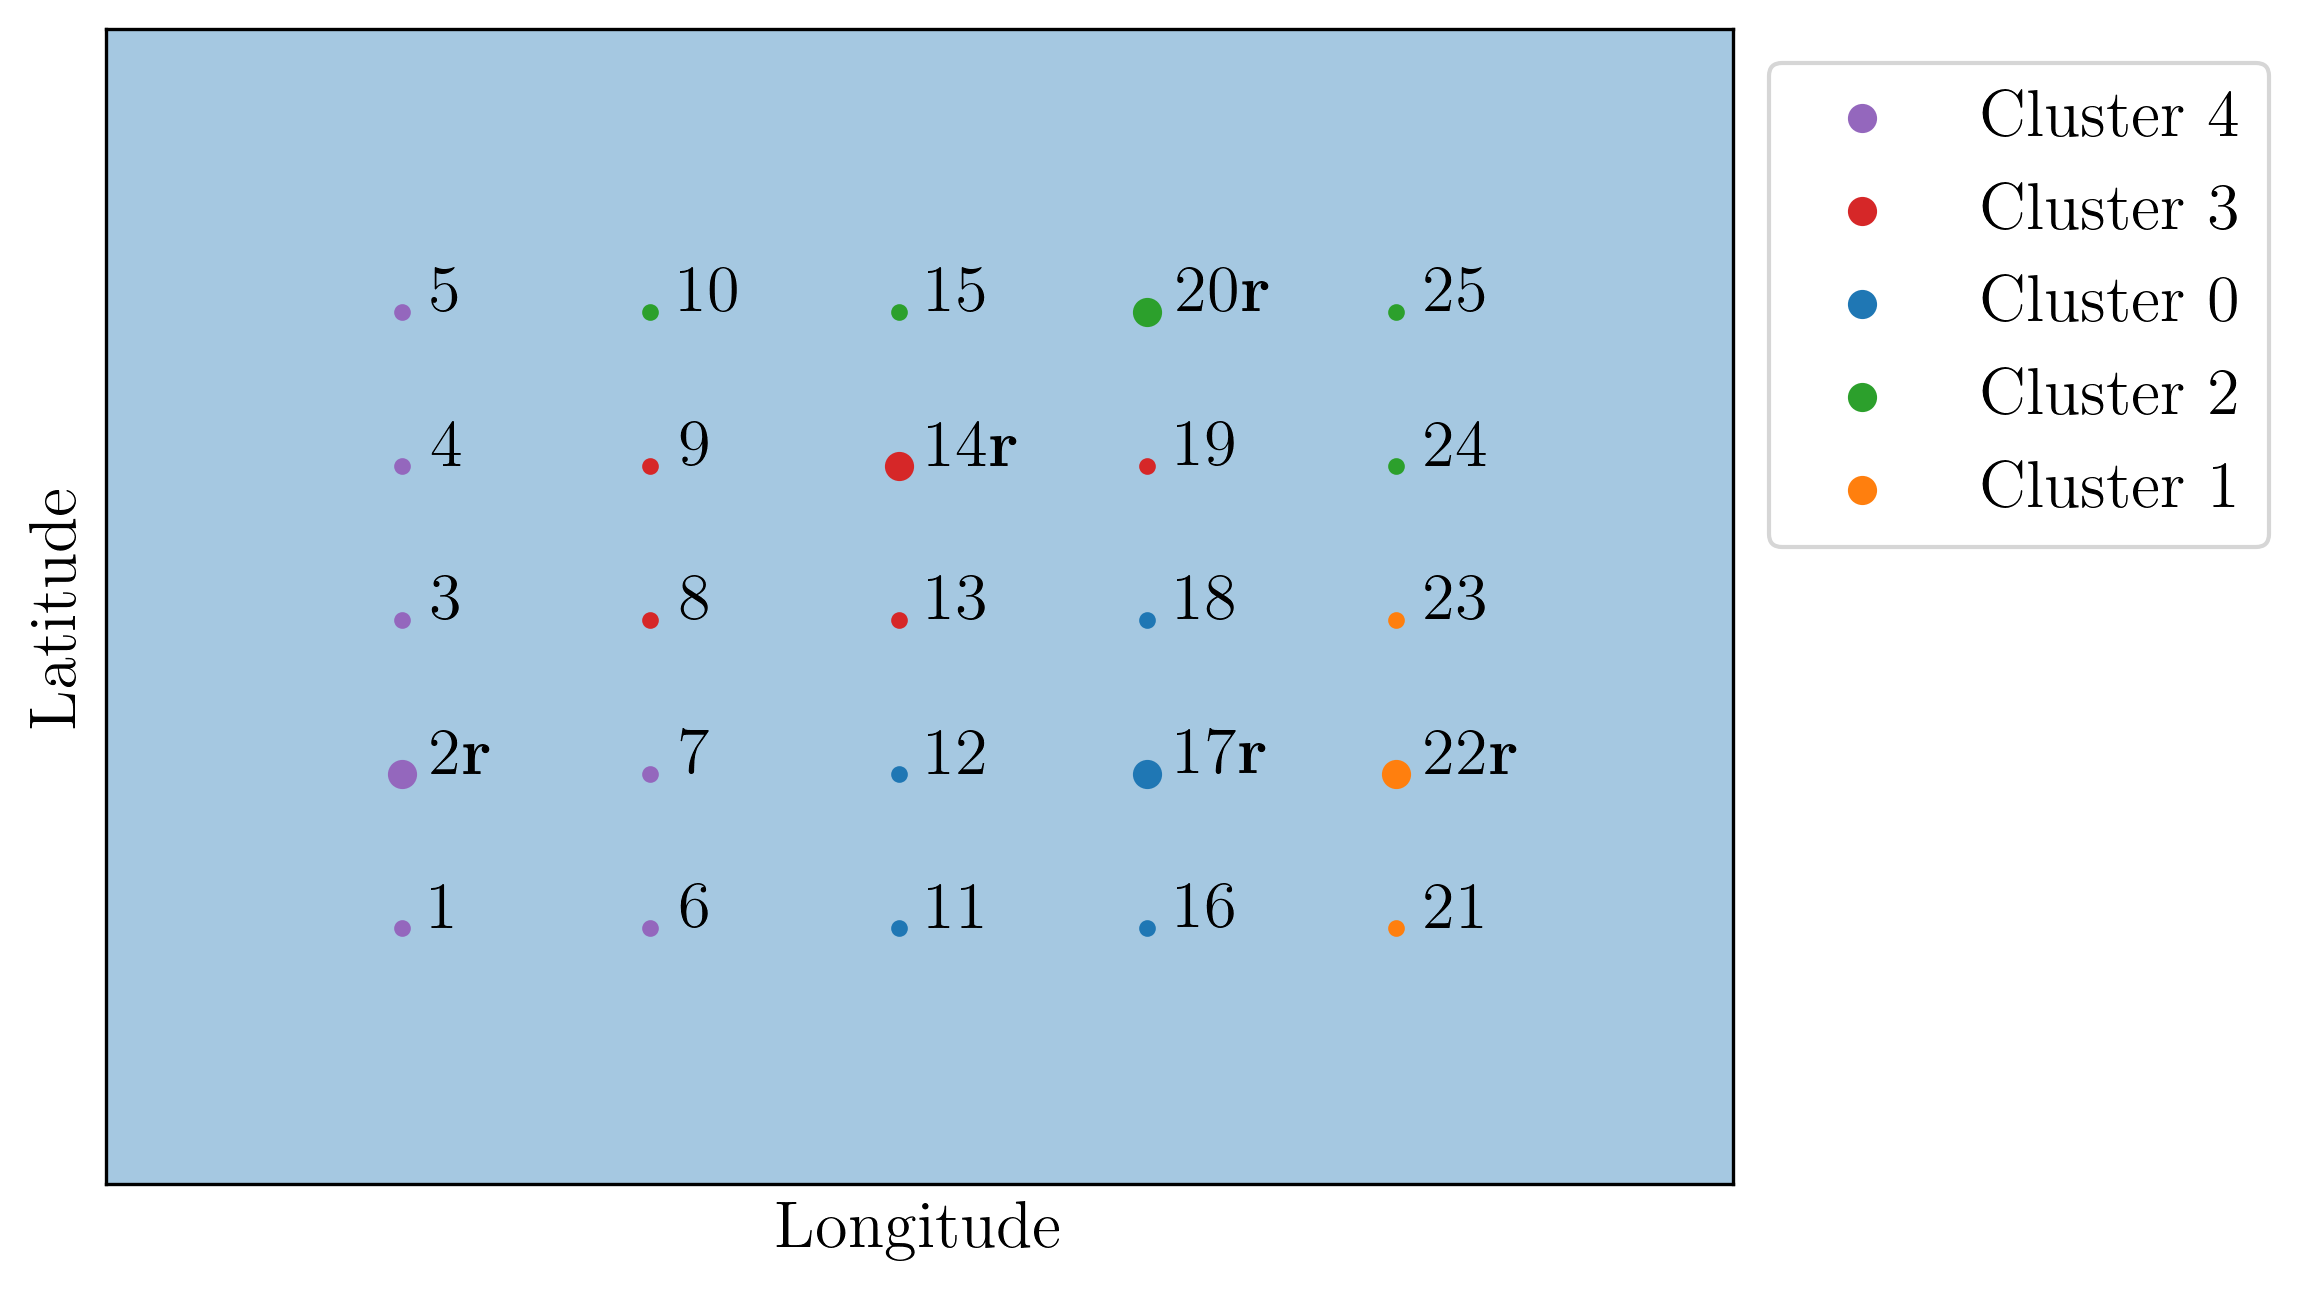
\includegraphics[width=0.6\textwidth]{part2/figures/WAKE/clusters_SB.png}
    \caption{K-medoids clustering solution for five clusters. The representative elements of the clusters are tagged with the mention ``r''.}
    \label{fig:kmedoids}
\end{figure}



%============================================================%
\subsection{Summary and discussion}
%============================================================%
This section studied the impact of the wake on the wind conditions in a farm. 
The ambient wind conditions were propagated on a low-fidelity wake model of a floating wind farm. 
Even if higher-fidelity models could simulate this phenomenon more accurately, their huge computational cost would not allow uncertainty propagation (e.g., several days for LES certain solver, with intensive parallelization). 
The present model has a reasonable error and has a short execution (i.e., about a few minutes on a regular computer). 
The resulting wake-perturbed distributions at each turbine were compared to each other using a kernel-based dissimilarity measure for distributions. 
Using this scalar metric of perturbations created by the wake, clusters were built.  
In the context of fatigue assessment at the farm scale, the computed clusters may reduce the computational effort by assessing one turbine per cluster.    


%============================================================%
%============================================================%
\section{Conclusion}
%============================================================%
%============================================================%

In this chapter, different aspects of uncertainty quantification were applied to define the metocean conditions in a wind farm. 
First, to infer a joint environmental distribution, a semiparametric approach was applied to a large dataset from a site in South Brittany, France. 
This semiparametric approach combines parametric models of the marginals with nonparametric models of the copula such as the highly flexible empirical Bernstein copula.  
Second, to take into account the heterogeneous wind conditions inside a farm, a dynamic wake meandering model was developed for the South Brittany farm. 
Then, the ambient joint environmental distribution was propagated through this model to recover a wake-perturbed environmental distribution per turbine.  

The copulogram is a new data visualization tool based on the empirical copula, aiming at improving the description of nonlinear dependencies in datasets.  

The maximum mean discrepancy is a kernel-based dissimilarity measure between multivariate distributions which was used throughout this chapter. 
Either for testing the goodness-of-fit of the semiparametric model fitted using the EBC, or as a measure of the perturbation occasioned by the wake on the wind conditions. 
In this context, the MMD allowed building clusters of turbines witnessing the same wind conditions. 
As perspectives, the robustness of this metric to the choice of kernel could be further investigated as well as the goodness-of-fit of the EBC over distributions' tails. 
After defining the probabilistic model of the environmental conditions, this uncertainty is ready to be propagated in a multiphysics wind turbine model as DIEGO. 
